\documentclass[a4paper,oneside,11pt]{article}
\usepackage{graphicx}
\usepackage{ tipa }
\usepackage{hyperref}
\usepackage{titling}
\usepackage{blindtext}
\usepackage{enumitem}
\usepackage{eurosym}
\usepackage{float}
\usepackage{listings}
\usepackage{tabularx}
\usepackage{alltt}
\usepackage[T1]{fontenc}
\usepackage{caption}
\usepackage{changepage}
\captionsetup[figure]{labelformat=empty}


\title{DD}
\author{Daniele Montesi, Nicola Fossati, Francesco Sgherzi}
\date{\today}
\begin{document}
    \begin{titlingpage} 
        \begin{center}
            
\includegraphics[height=5cm]{assets/Logo_Politecnico_Milano.png}\\
            \vspace{4cm}
            \begin{huge} 
                \textbf{\thetitle} \\
            \end{huge}
            \vspace{0.3cm}
            \begin{Large}
                \textit{Software Engineering 2 Project - TrackMe} \\
            \end{Large}
        \end{center}
        \begin{large}
            \vspace{4cm}
            \textbf{Authors}
            \begin{itemize}
                \item Daniele Montesi - \textit{912980} 
                \item Nicola Fossati - \textit{915244}
                \item Francesco Sgherzi - \textit{915377}
            \end{itemize}
        \end{large}
    \end{titlingpage}
    \newpage
    \tableofcontents
    \newpage
    \section{Introduction}
    
        \subsection{Purpose}
            The main purpose of this document is to exhaustively describe the Data4Help main architecture, its parts and how they interact. There is also a chapter that covers the user interface.

The main recipients of this document are the project manager, developers and testers, but it can also be useful for further development reference and maintenance.
        \subsection{Scope}
            % To define the scope of the product we can use ``The World \& Machine'' approach by M. Jackson and P. Zave.
% We can define the real world entities that interact with the system (the World), the entities that belong to the system (the Machine) and the shared phenomena (the intersection of the two other sets).

% TODO: add image here

The \textit{The World and the Machine} approach is used in defining the scope of the project.
By defining the real world entities that interact with the system and the properties of the system itself we can determine the intersection between the two sets: the \textit{shared phenomena}.
\begin{center}
    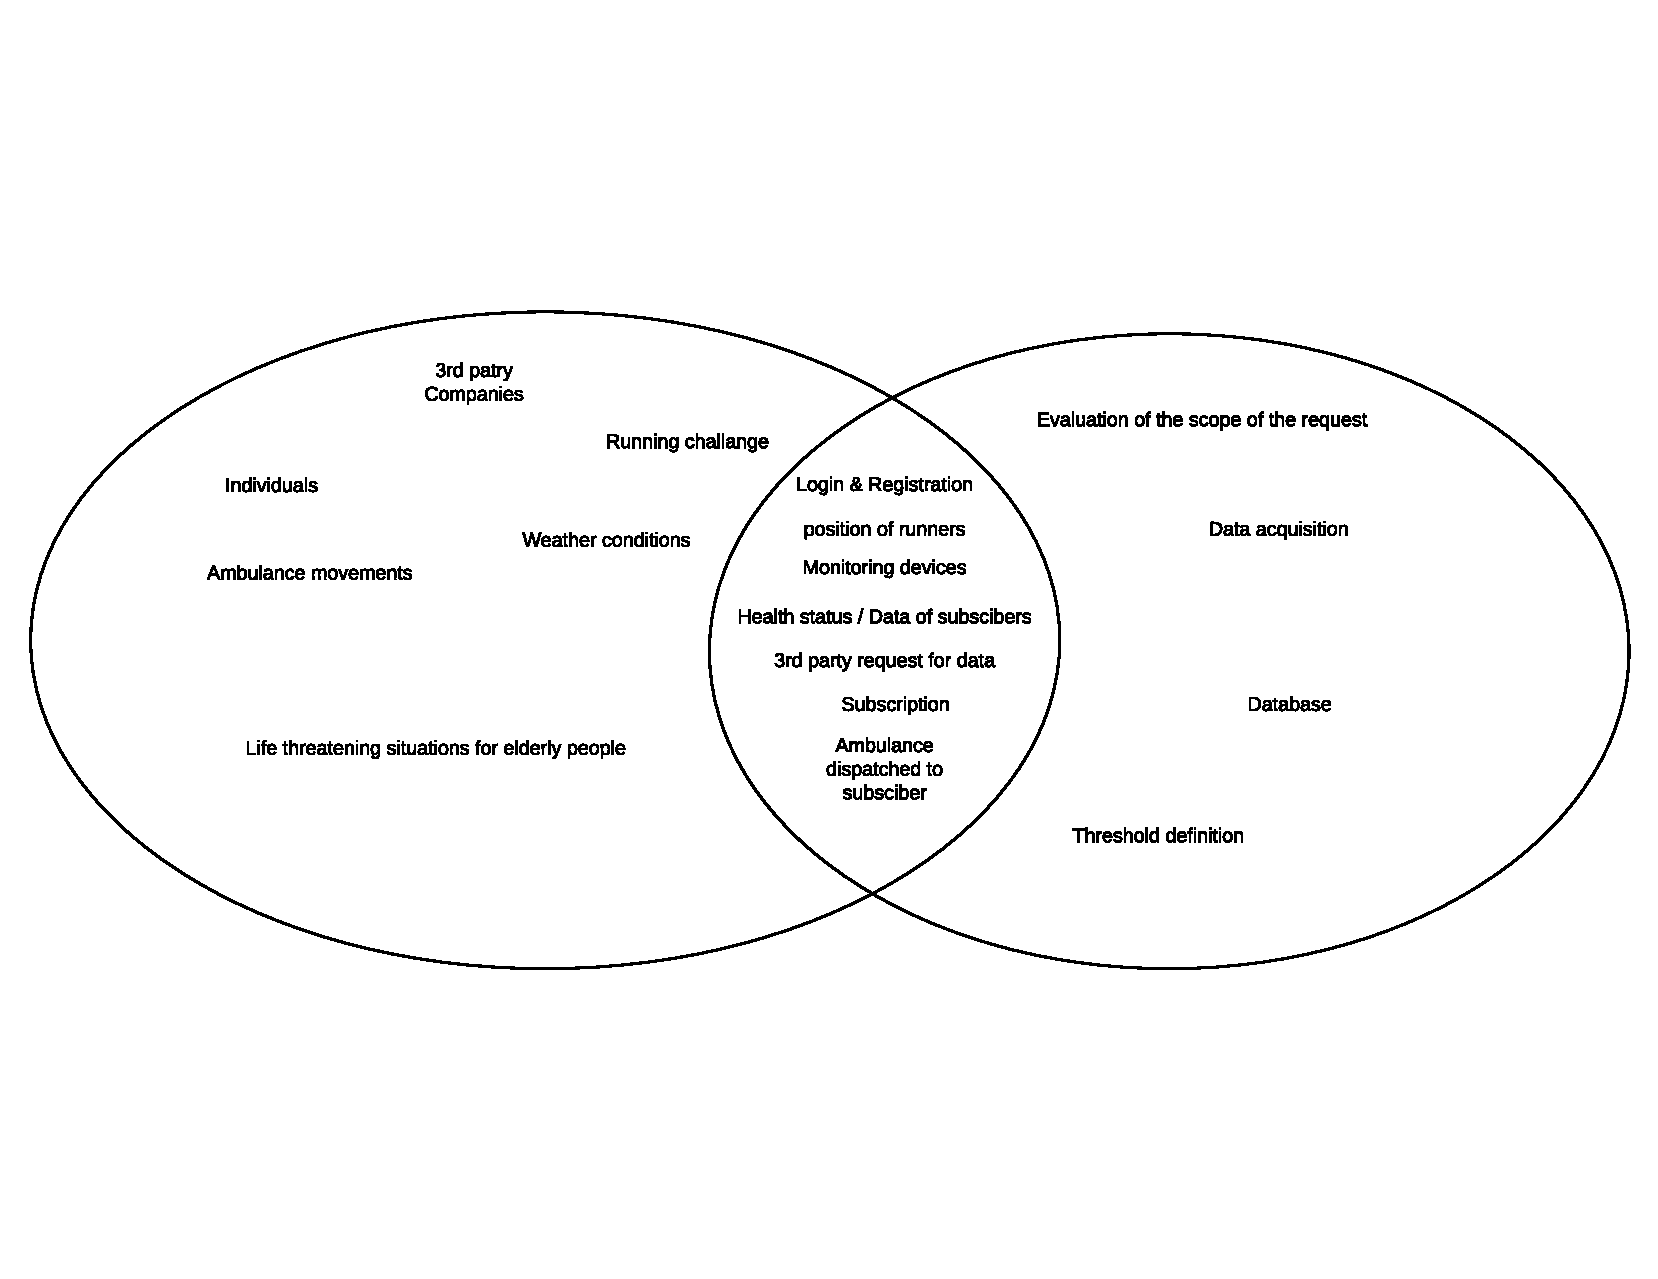
\includegraphics[height=8cm,keepaspectratio]{assets/twatm.pdf}
\end{center}

The system-to-be uses 3 components with different roles in order to work:
\begin{itemize}
    \item \textbf{Data4Help SmartWatch App}: Acquires the data from the smartwatch sensors (heart rate, sleep quality, position, phisical activities) and sends them via Bluetooth to the Data4Help Mobile App
    \item \textbf{Data4Help Mobile App}: Gathers data from the smartwatch, shows various statistics, and sends them to the Data4Help Core Database. Each user can choose which service subscribe to
    \item \textbf{Data4Help Website}: Gives third-party companies the ability to request data, either anonymized or user specific. Moreover, it allows run organizers to define the path of the run and the spectators to see the position of all runners on a map.
    \item \textbf{Data4Help Core}: is intended to connects all other components together providing the logic of the application. It is also responsible for the acceptance of all third-parties requests of data. It also evaluate health status of individuals deciding whether is at risk or not.
\end{itemize}

The list below shows the main goals the system should be able to accomplish:

\begin{itemize}
    \item \textbf{G1}: The system should be able to read sensor data from smart devices.
    \item \textbf{G2}: The system should be able to show acquired data via the Mobile App and the Website.
    \item \textbf{G3}: The system should allow users to register.
    \item \textbf{G4}: The system should allow companies to register.
    \item \textbf{G5}: The system should allow registered companies to request data either from specific individuals or from an anonymized group of individuals.
    \item \textbf{G6}: The system should allow users to accept or decline a company request for their specific data.
    \item \textbf{G7}: The system should provide a payment method to registered companies requesting user data. %eviterei di specificare payment system
    \item \textbf{G8}: The system should be able to communicate directly to ambulances.
    \item \textbf{G9}: The system should be able to react to the lowering of the health parameters below threshold in less than 5 seconds and send the position of the person to the ambulance system. 
    % \item \textbf{G10}: The system should should allow organizers to define the path for the run.
    \item \textbf{G10}: The system should be able to communicate interoperably with its services: \textit{AutomatedSOS} and \textit{Track4Run}
    \item \textbf{G11} The system should allow run organizers to register.
    \item \textbf{G12} If a run organizer is registered, it can define a run i.e. it can define the path that the participants should follow.
    \item \textbf{G13} A user should be able to enroll to a run.
    \item \textbf{G14} Spectators of a run should be able to see each participant's position on a map.
\end{itemize}

%A health data aggregator app that gives the user the ability to monitor all 

%is intended to offer all the functionalities of the service to the individuals, including heart rate monitoring, sleep monitoring




        \subsection{Definitions, Acronyms, Abbreviations}
            \renewcommand{\arraystretch}{1.5}
\begin{center}
    \begin{tabular}{|l|r|}
        \hline
        \textbf{i.e.} & \textit{Id est}, that is  \\
        \hline
        \textbf{w.r.t} & with respect to  \\
        \hline
        \textbf{w.l.o.g.} & without loss of generality \\
        \hline
        \textbf{The company} & TrackMe \\
        \hline
        \textbf{BLE} & Bluetooth Low Energy \\
        \hline
    \end{tabular}
\end{center}
        \subsection{Revision history}
        \subsection{Reference documents}
            \begin{itemize}
\item \textbf{|REFD1|} \href{https://en.wikipedia.org/wiki/Model–view–presenter}{\textbf{MVP}}

\item \textbf{|REFD2|} \href{https://standards.ieee.org/standard/1016-2009.html}{\textbf{IEEE Std 1016-2009 Standard for Information Technology, Systems Design, Software Design Descriptions}}

\item \textbf{|REFD3|} \href{https://it.wikipedia.org/wiki/Representational_State_Transfer}{\textbf{Representational State Transfers}}

\end{itemize}
        \subsection{Document structure}
        This document is divided in the following chapters:
\begin{description}
\item[Implemented requirements] Explains which functional requirements outlined in the RASD are accomplished, and how they are performed.
\item[Design choices] provides reasons about the implementation decisions taken in order to develop the application.
\item[Source code structure] explains and motivates how the source code is structured both in the front end and in the back end.
\item[Testing] provides the main testing cases applied to the the application
\item[REST API] describes the API implemented for the application.
\end{description}
    
    \newpage
    \section{Architectural Design}
        \subsection{Overview}
            This section is intended to explain in detail all the components used by the system in order to offer all the functionalities.

The figure above shows the high-level architecture of the system-to-be. 
All the components are better explained in the following paragraph.

CLIENTS:
Mobile App Clients (Smartwatch App Clients), Web Client 

Application server

Data (Choose)

\begin{figure}[H]
	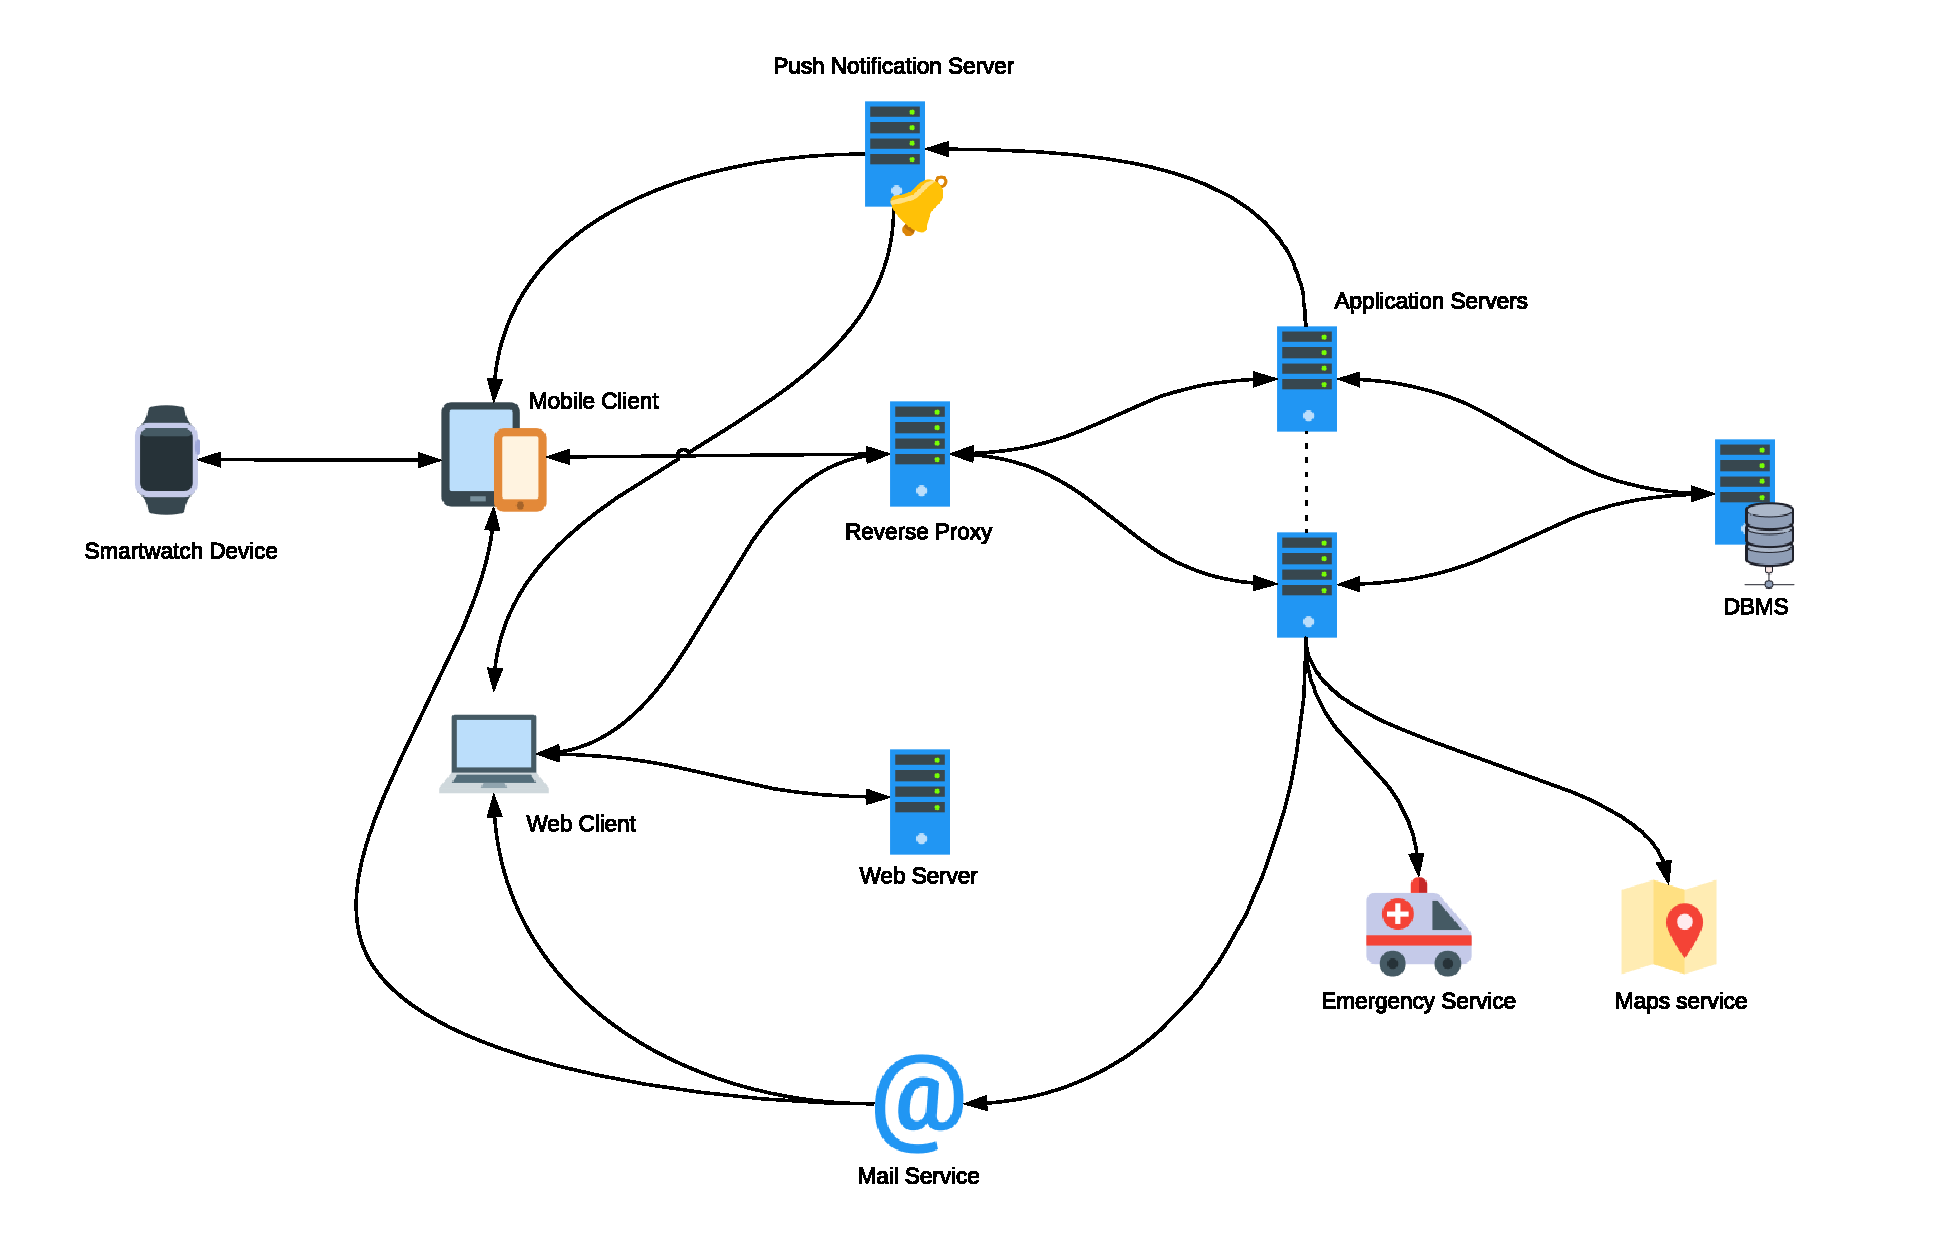
\includegraphics[width=\textwidth,height=\textheight,keepaspectratio]{assets/ArchitecturalDesignOverview.pdf}
	\caption{System overview graph}
	\label{fig:SOG}
\end{figure}

        \subsection{Component view}
            \begin{figure}[H]
	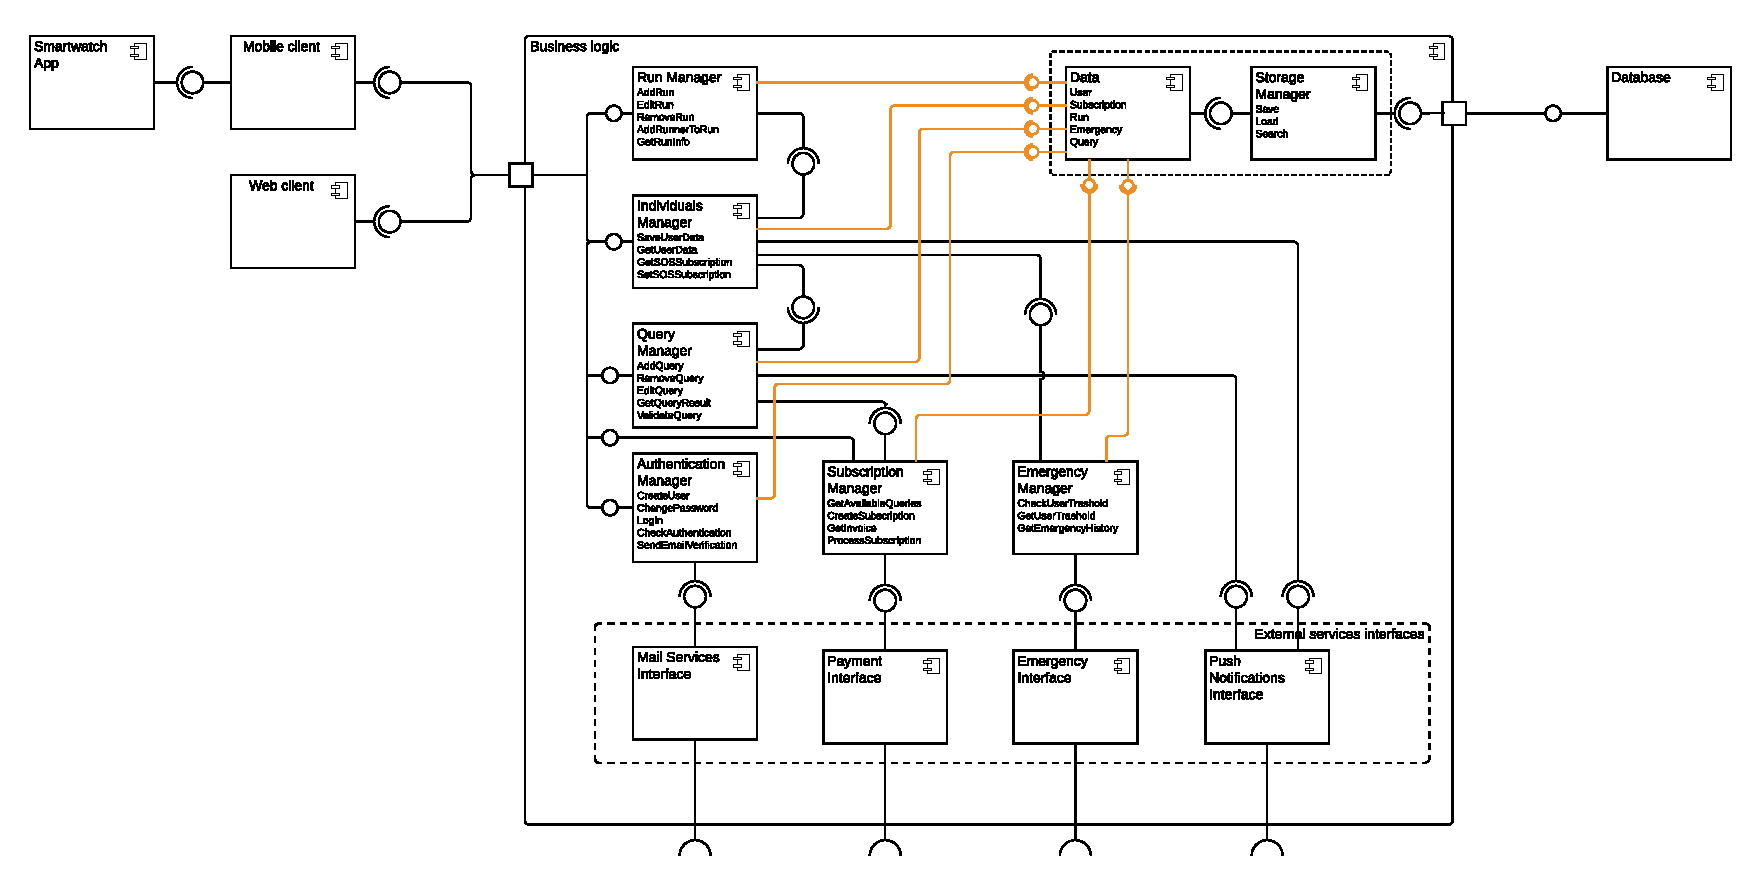
\includegraphics[width=\textwidth,height=\textheight,keepaspectratio]{assets/ComponentDiagram.pdf}
	\caption{Component Diagram}
	\label{fig:CD}
\end{figure}


\noindent The picture shows the components of the application divided in Client, Business Logic and Data tier.

\noindent Below are described more in detail all the components and interfaces that the system uses to offer its functionalities.

\paragraph{Smartwatch device} \mbox{} \newline
The Smartwatch device is directly connected to the mobile app of the user and does not interact with the business logic.
Data coming from the sensors of the smartwatch are sent to the mobile app via bluetooth.

\paragraph{Mobile client and Web client} \mbox{} \newline
The clients of the system.
\begin{itemize}
    \item The Mobile client is used by individuals that want to exploit the services of Data4Help.
    \item The Webclient is used by Companies that want to exploit the query services of Data4Help.
\end{itemize}


\paragraph{Individuals Manager} \mbox{} \newline
The Individuals manager has to 
\begin{itemize}
    \item notify the system when there are new data available and store them into it;
    \item manage user requests for historical data, accessing Data4help database;
    \item ask the user if he agrees to be monitored by a company that has requested an individual query, sending him a push notification;
    \item communicate data to Emergency manager (only if user is subscribed to AutomatedSOS);
\end{itemize}


\paragraph{Authentication Manager} \mbox{} \newline
The component that manages users log-in and registration and is in charge of:
\begin{itemize}
    \item allowing user login;
    \item changing user authentication information;
    \item adding new user to database;
    \item communicating with Email interface in order to send verifications request to the user
\end{itemize}

\paragraph{Query Manager} \mbox{} \newline
The core component of the Business unit. It is in charge of:
\begin{itemize}
    \item \textbf{Get query results};
    \item \textbf{Validating queries}: verify if there is a sufficient number of users involved in the scope of the query (in case of a query on group of individuals), and if a company is allowed to do a query according to its payment subscription;
    \item \textbf{Adding queries} to a company account;
    \item \textbf{Deleting queries} from a company account that wish to unsubscribe
    \item \textbf{Updating queries}, when a company has subscribed to a query and wants to edit its query; interacts with the Push Notification interface to send the "New data" notification.
\end{itemize}

\paragraph{Subscription Manager} \mbox{} \newline
The component is in charge of managing the subscription of companies to a payment plan offered by Data4Help.
It has to:
\begin{itemize}
    \item \textbf{Subscribe}: let companies subscribe to new payment plans;
    \item \textbf{Store} in the database subscriptions of every company;
    \item \textbf{Let companies see} their subscription detail;
    \item \textbf{Interact} with the payment service to let company pay for subscriptions.
\end{itemize}



\paragraph{Emergency Manager} 
\mbox{} \newline
The component is in charge of 
\begin{itemize}
    \item \textbf{Evaluating} user health parameters;
    \item \textbf{Store} in the database threshold parameters for users subscribed to AutomatedSOS;
    \item \textbf{Checking} when a parameter of a user goes below the threshold. If so, the component is in charge to communicate with ambulance API throughout the Emergency interface.
\end{itemize}


\paragraph{Run Manager} \mbox{} \newline
The component is in charge of:
\begin{itemize}
    \item \textbf{Creating races}: allows run organizers to create new races;
    \item \textbf{Listing run}: provides a list of runs be available to users;
    \item \textbf{Adding} new runners to a race;
    \item \textbf{Managing}: let run organizers manage a race's information.
\end{itemize}


\paragraph{External services interface} \mbox{} \newline
The system has 3 interfaces components that are in charge of communicating with the external services API.
The interfaces are:
\begin{itemize}
    \item Push Notification Interface: communicates with a push notification server API in order to send notifications to mobile client;
    \item Emergency Services Interface: communicates with Ambulance API provided by Hospitals in order to send an ambulance if the user health parameters go below thresholds;
    \item Mail Services Interface: communicates with email server to send email.
    \item Payment Interface: communicates an external payment service in order to create payment requests and validate them.
\end{itemize}

The diagram below describes in details the components and the entities of the application server.


\begin{figure}[H]
	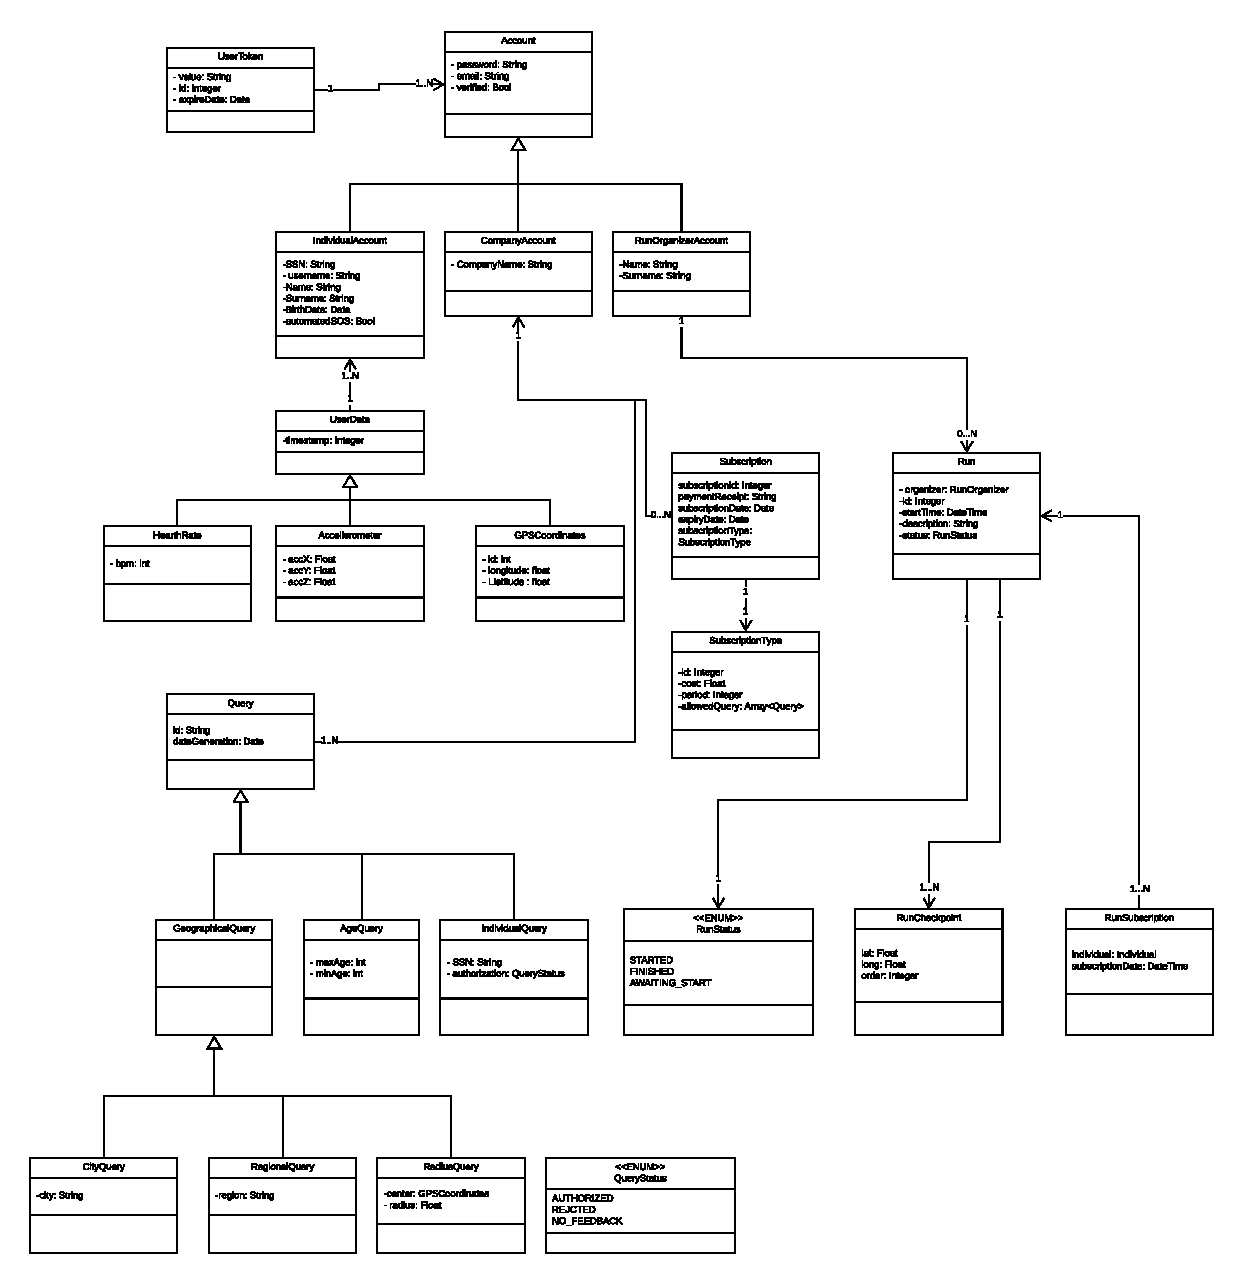
\includegraphics[width=\textwidth,height=\textheight,keepaspectratio]{assets/UML_Entities.pdf}
	\caption{Entities diagram}
	\label{fig:UMLEntityDiagrams}
\end{figure}

        \subsection{Deployment view}
            The diagram shows the deployment of the system and its structure.

\begin{figure}[H]
	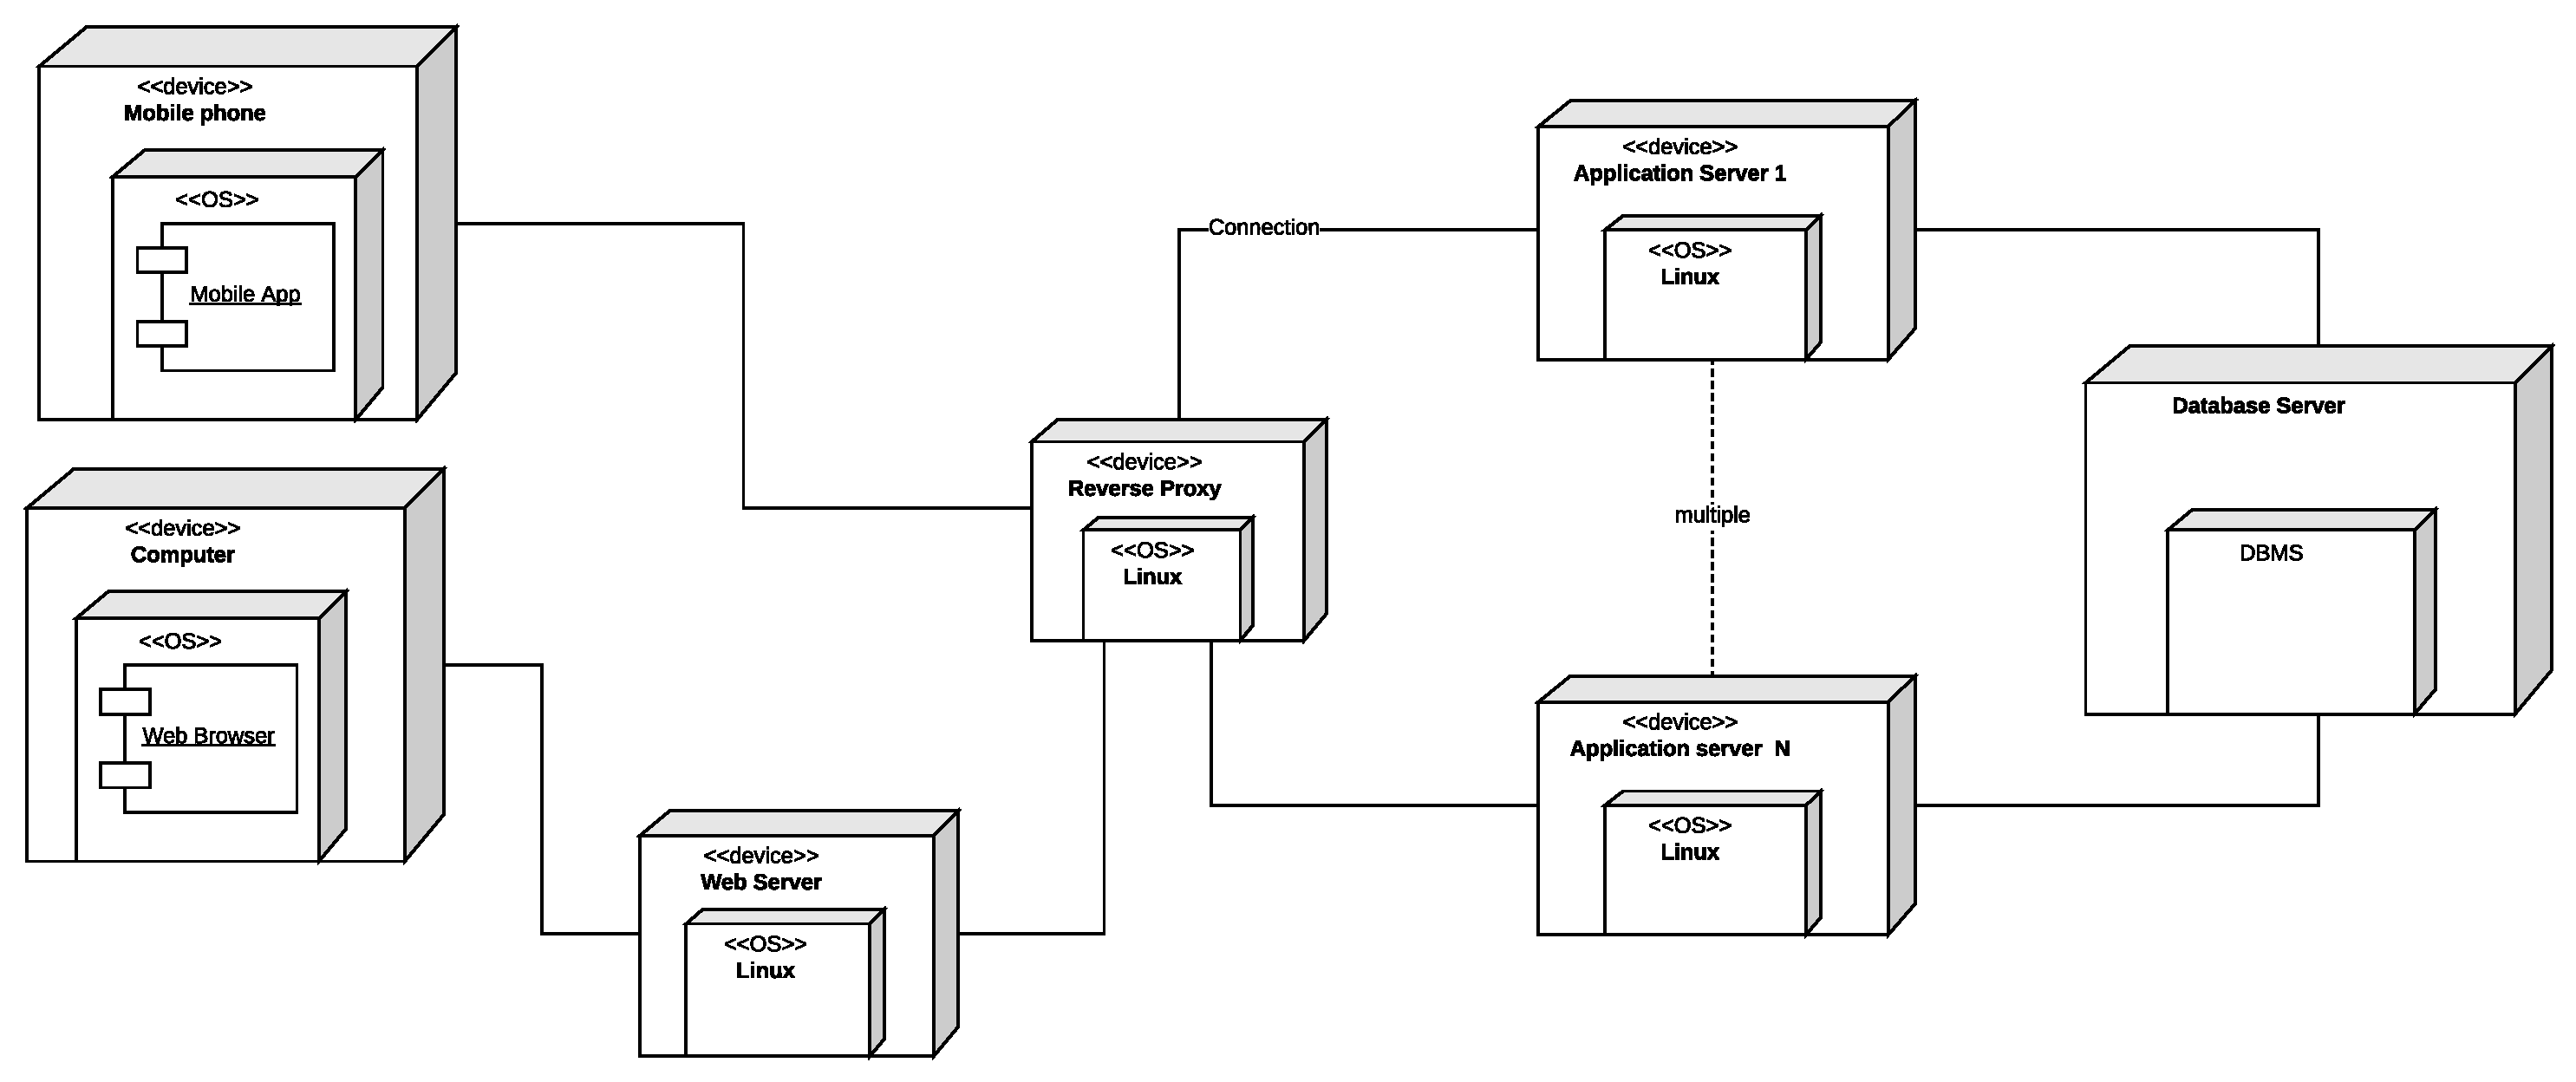
\includegraphics[width=\textwidth,height=\textheight,keepaspectratio]{assets/DeploymentDiagram.pdf}
	\caption{Deployment diagram}
	\label{fig:DD}
\end{figure}

\begin{itemize}
    \item \textbf{Client}: represents the first layer. We distinguish between 2 typologies of clients: Web Browser and Mobile app.
    \item \textbf{Server}: is part of the second layer. 
    We distinguish:
    \begin{itemize}
        \item Application server: contains all the business logic of the system.
        \item Web Server: contains the data concerning to the web pages
    \end{itemize}
    \item \textbf{Reverse proxy}: is part of the second layer of the system.
    Is a type of proxy server that retrieves resources on behalf of a client from one or more servers.
    \item \textbf{Database}: is the third layer of the system that stores all the data. 
    The system uses a relational DBMS.
\end{itemize}

        \subsection{Runtime view}
            \subsubsection{User registration}
Each individual should register an account in order to use the System. The user initially fills a form on its smartphone providing all the required data. The Mobile App also collects the model of the smartwatch. \\
This data is sent over the internet, using an HTTP POST request to the AuthenticationManager, with all the required data in JSON format. The AuthenticationManager firstly checks if the smartatch is compatible. If it is, it checks that the email and SSN/fiscal code are not used by any individual already registered. If all the check pass an Individual and an Account are created in the database.\\
The account initially is not confirmed.\\
Then, a mail is sent to the email provided, with a verification code.
When the user inserts the verification code in the app, an HTTP POST request is made to the System and the user, if the code is correct, is put in the active state.
\begin{figure}[H]
	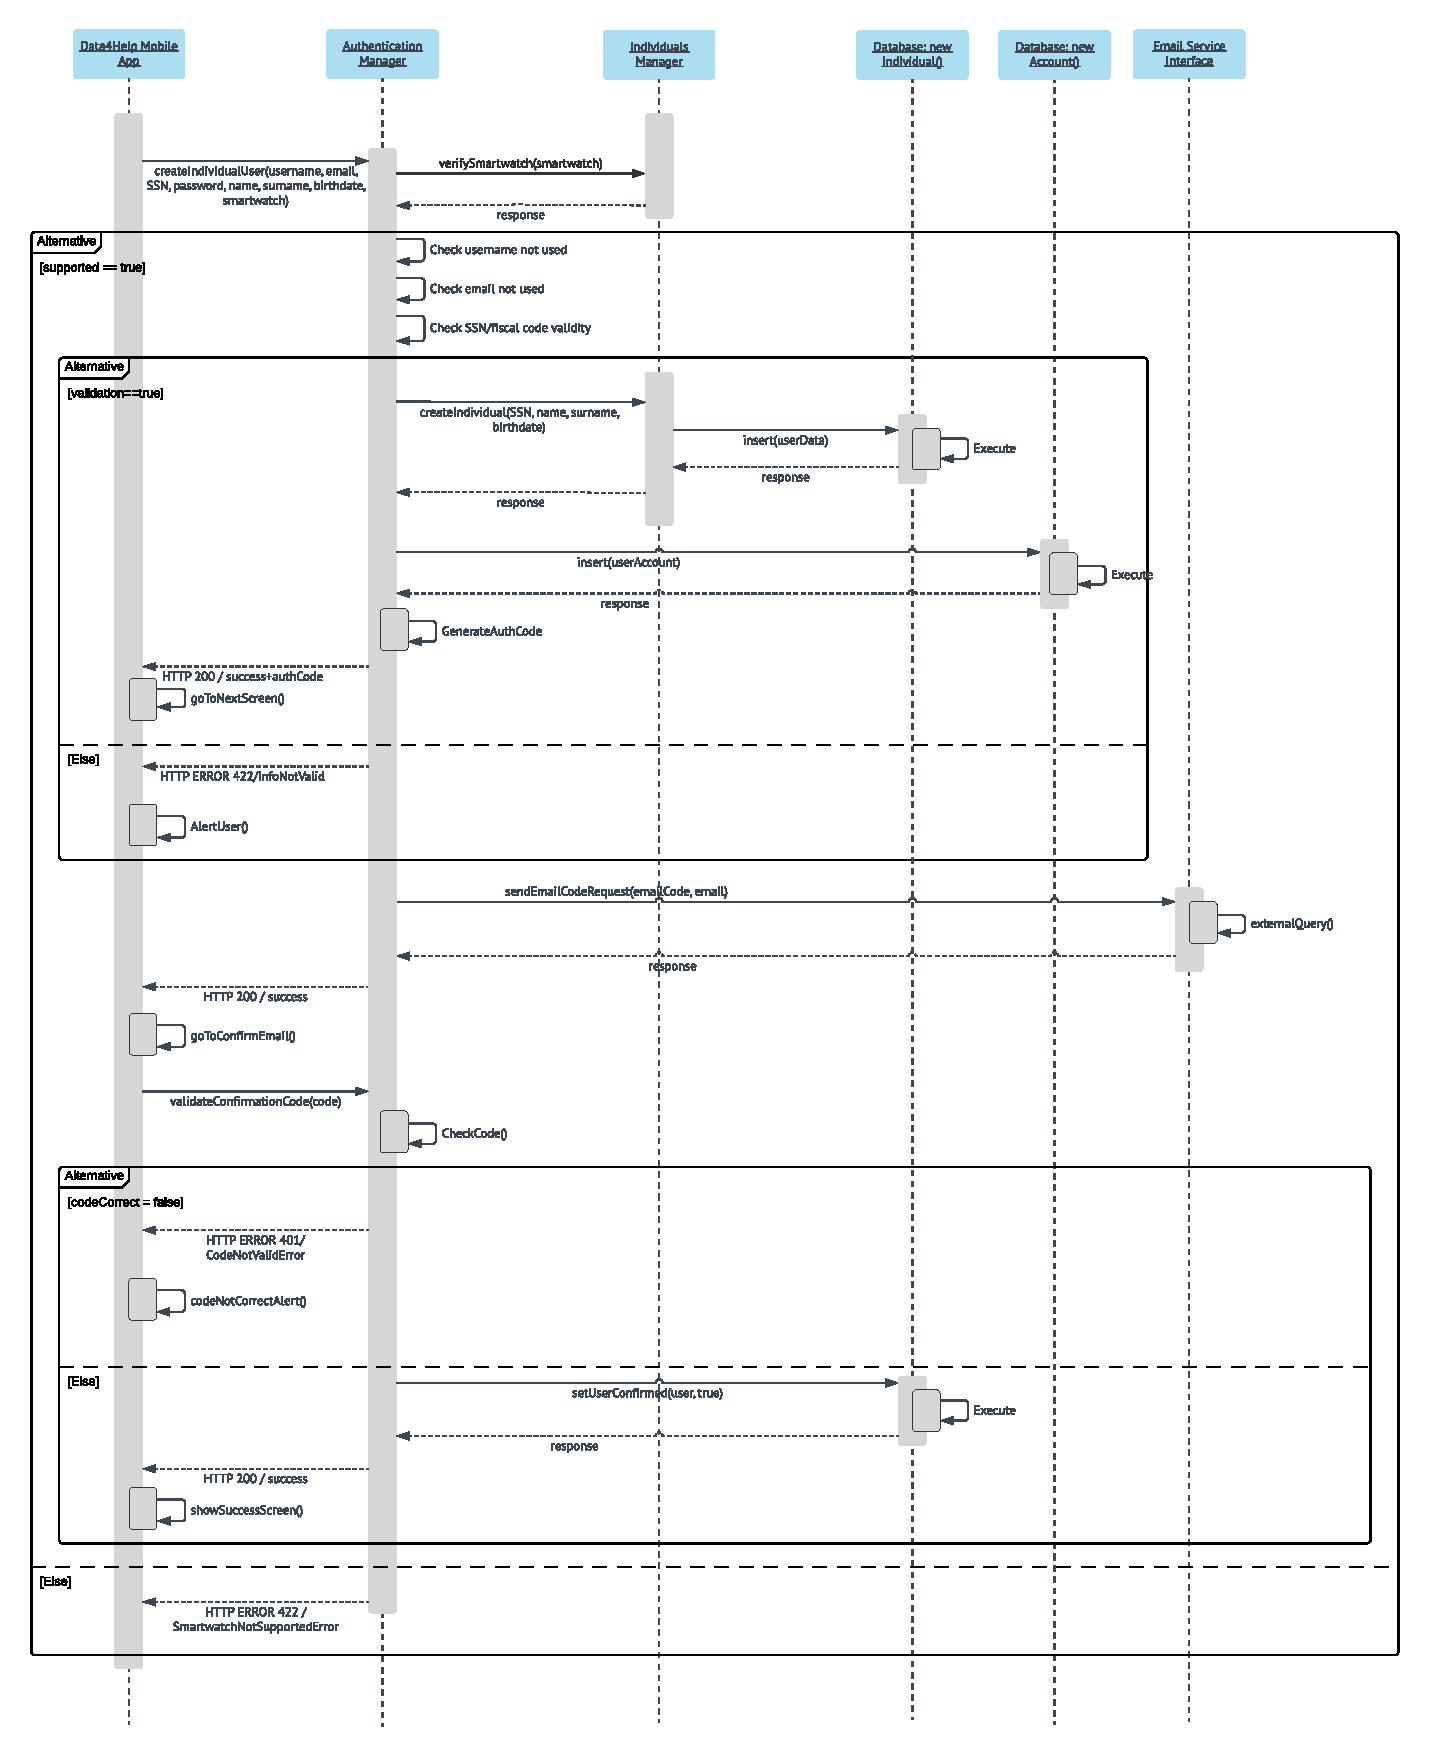
\includegraphics[width=\textwidth,height=\textheight,keepaspectratio]{assets/flowCharts/IndividualRegistration.pdf}
	\caption{User registration Runtime View}
	\label{fig:IndividualRegistration}
\end{figure}


\subsubsection{General Login}
When a generic user (one among Individual, Company or Run organizer) wants to login, an HTTP POST request is made to the authentication manager. It checks if the username and password combination are correct.\\
If they are, it generates an authToken, stores it in the database and then returns it to the caller.
The caller can use this authentication token for each subsequent call; the token will remain valid for 24 hours.
\begin{figure}[H]
	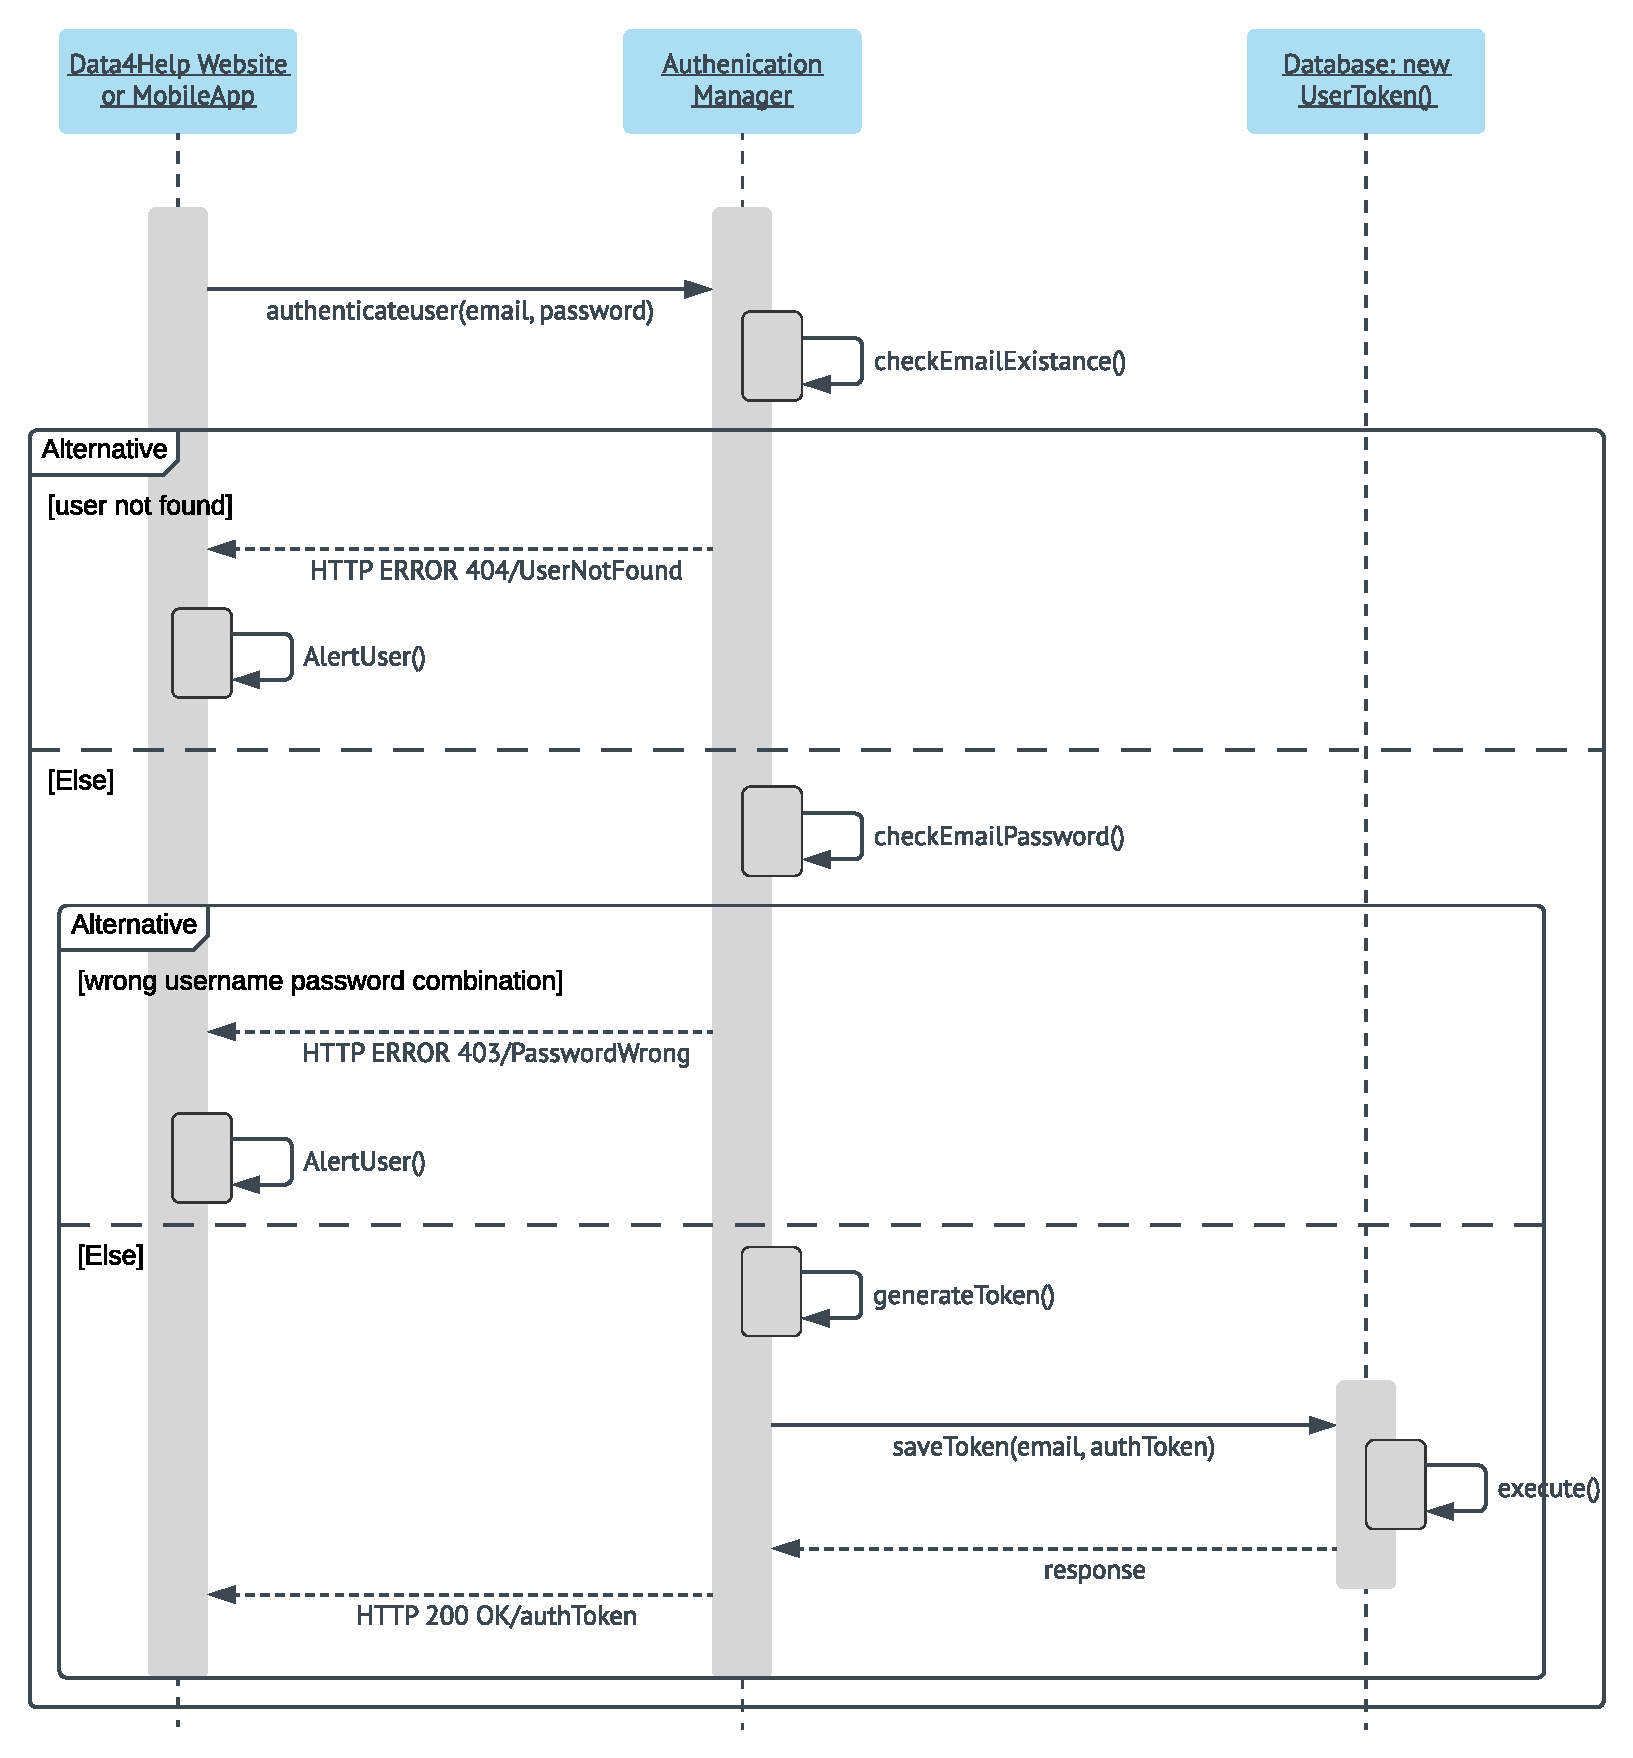
\includegraphics[width=\textwidth,height=\textheight,keepaspectratio]{assets/flowCharts/UserLogsIn.pdf}
	\caption{General Login Runtime View}
	\label{fig:UserLogsIn}
\end{figure}



\subsubsection{Consulting Individual Activity History}
When an Individual wants to look at its activity history, the app makes an HTTP GET request to the IndividualManager, including, beside the auth code, the begin date, the end date and the parameter type that he wants to get. \\
After checking the token, the IndividualManager gets the SSN and then looks for the data requested in the database. Then it returns the data found to the caller.
\begin{figure}[H]
	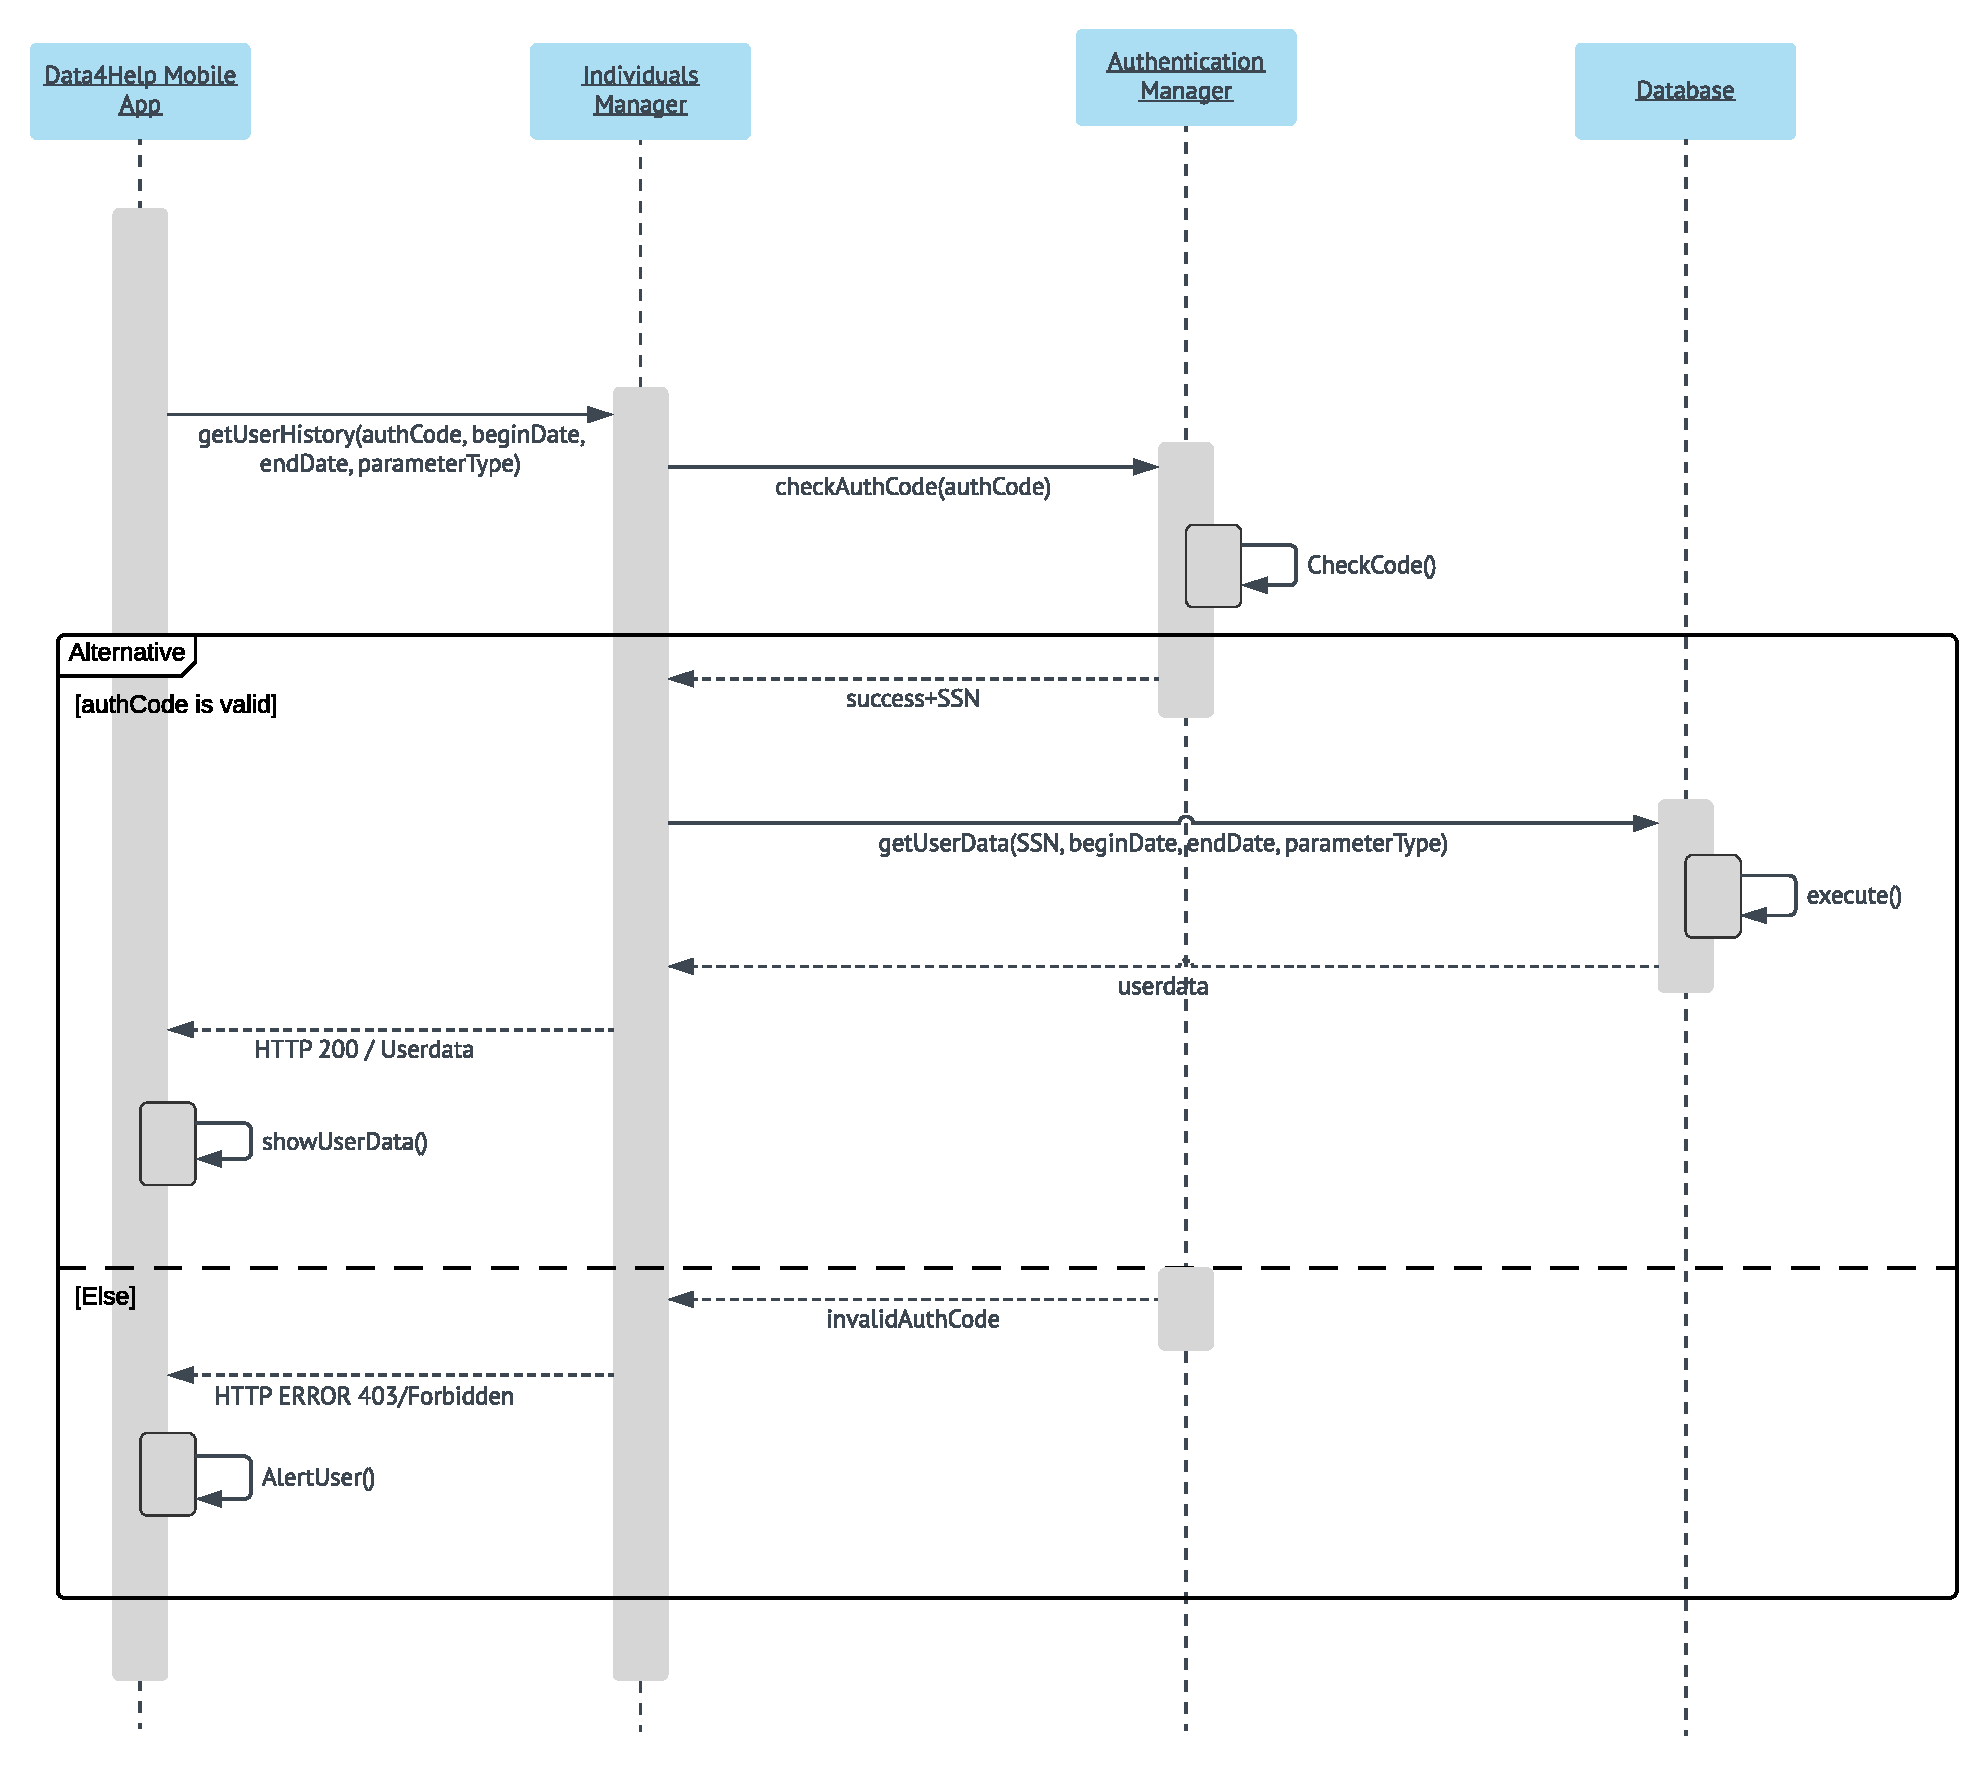
\includegraphics[width=\textwidth,height=\textheight,keepaspectratio]{assets/flowCharts/ConsultingIndividualActivityHistory.pdf}
	\caption{Consulting Individual Activity History Runtime View}
	\label{fig:ConsultingIndividualActivityHistory}
\end{figure}

\subsubsection{Data Synchronization}
When the bluetooth is activated, the Mobile App tries to enstabilish a connection with the Smartwatch App. When the connection is enstabilished, the Mobile App tries to get new data from the Smartwatch. If there is new data, it gets it and send it to IndividualManager through an HTTP POST request, alongside with the authToken perviously obtained. If the authToken is correct, the IndividualManager saves the data and then makes a call to checkUserTreshold in EmergencyManager and notifyCompanies in QueryManager.
\begin{figure}[H]
	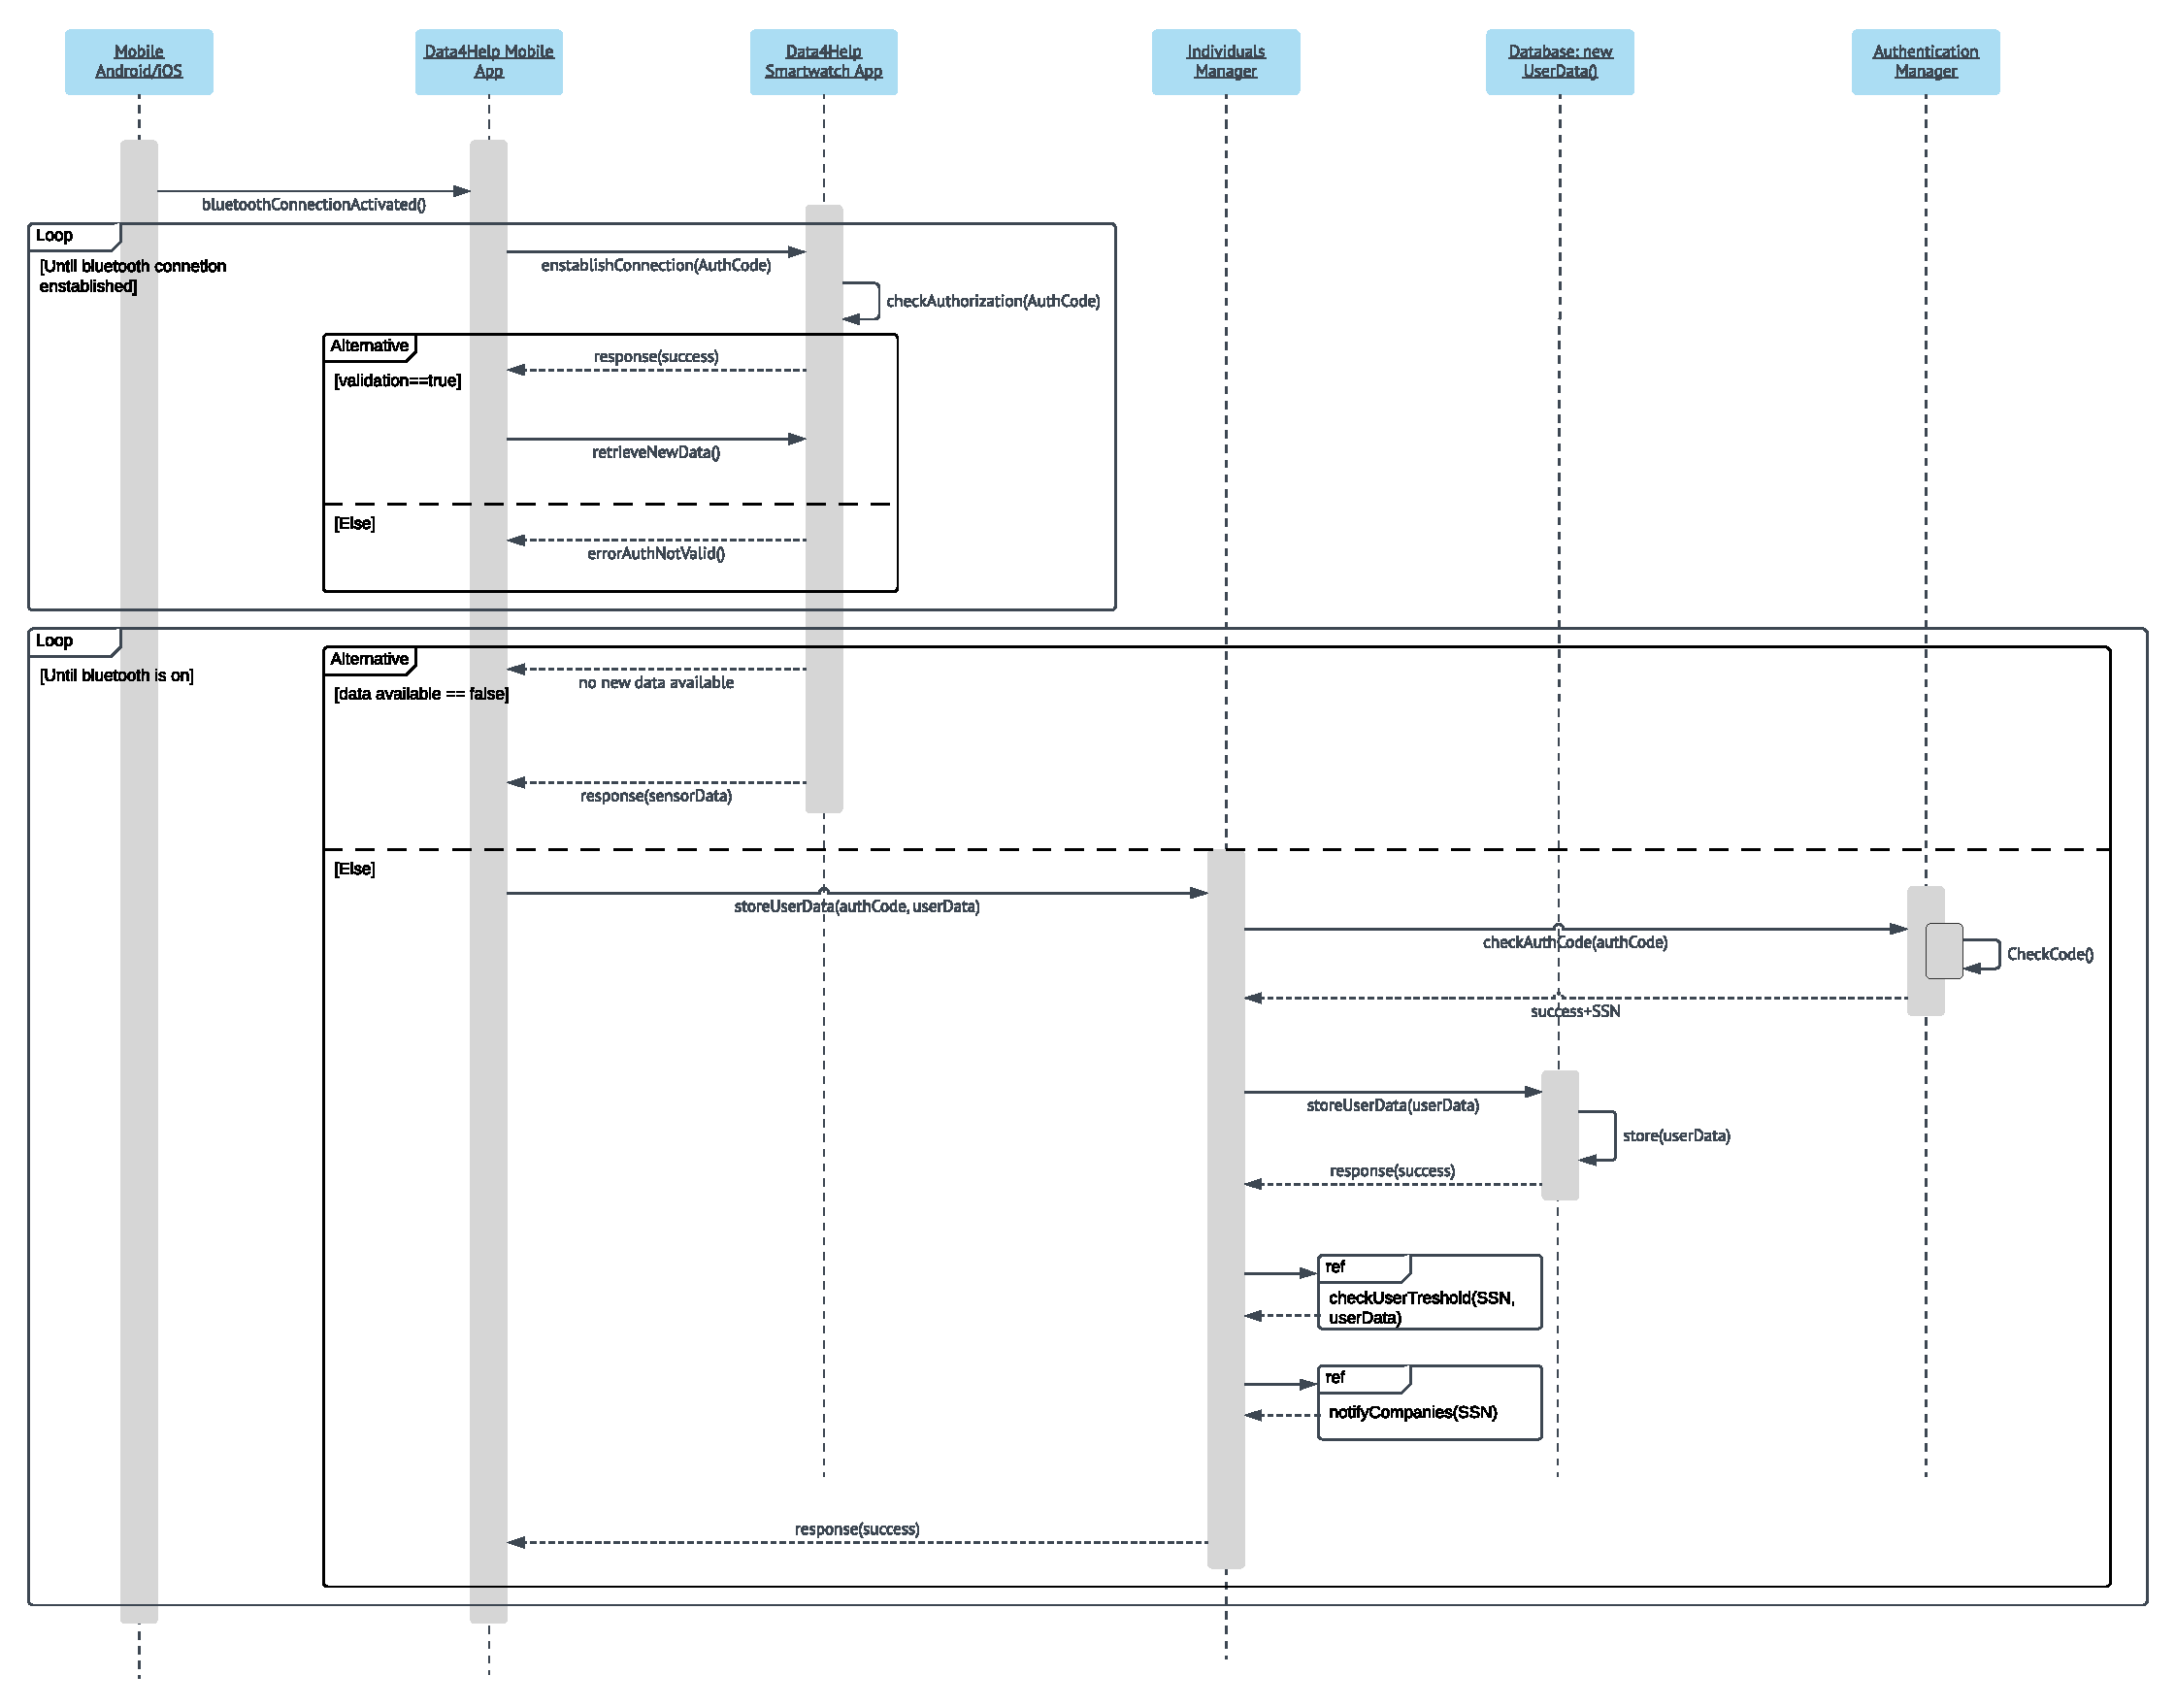
\includegraphics[width=\textwidth,height=\textheight,keepaspectratio]{assets/flowCharts/DataSynchronizationSmartwatchSmartphone.pdf}
	\caption{Data Synchronization Runtime View}
	\label{fig:DataSynchronizationSmartwatchSmartphone}
\end{figure}

\subsubsection{Company Registration}
The flow is the same as per the user regstration, excluding that the smartwatch is not checked and the user is only created in the AuthenticationManager database.
\begin{figure}[H]
	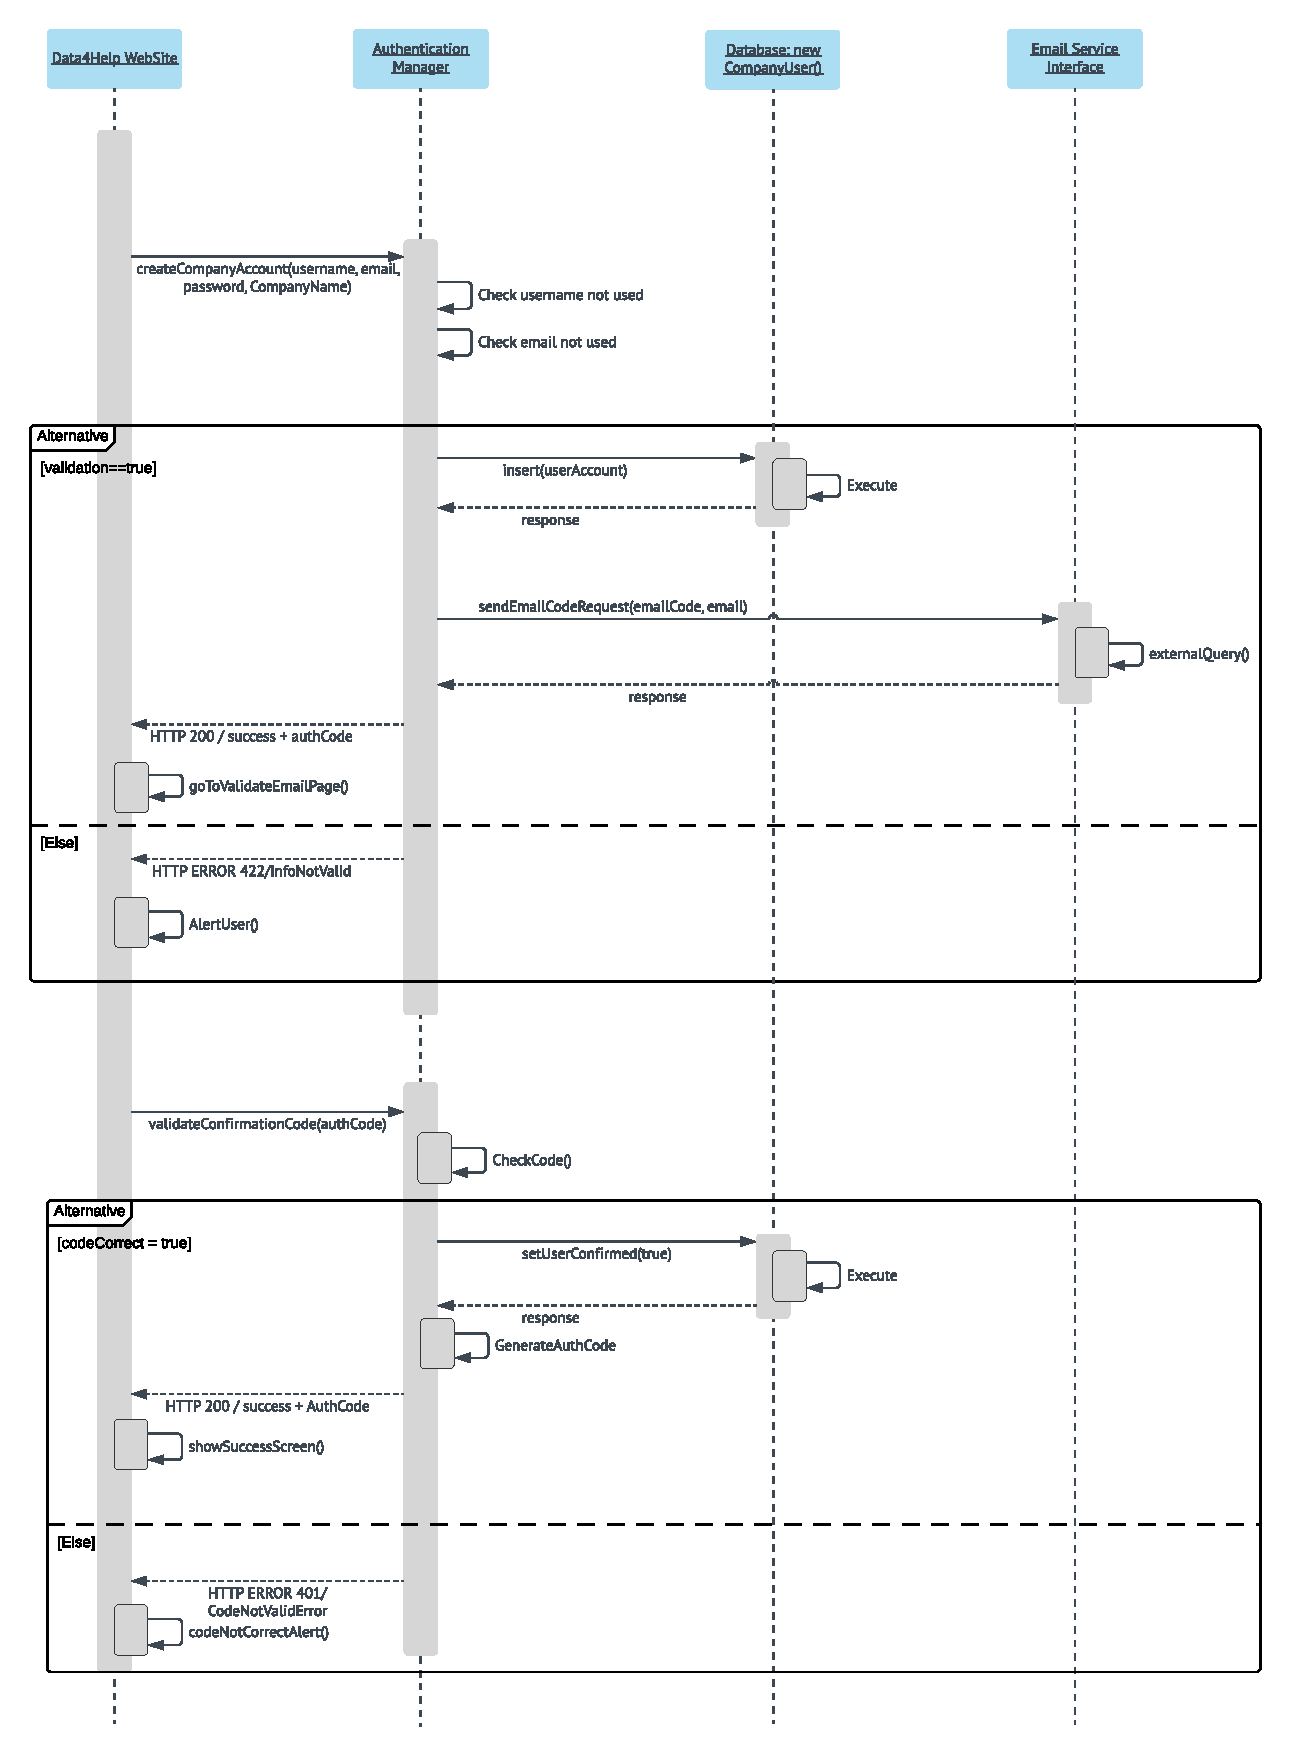
\includegraphics[width=\textwidth,height=\textheight,keepaspectratio]{assets/flowCharts/CompanyRegistration.pdf}
	\caption{Company Registration Runtime View}
	\label{fig:CompanyRegistration}
\end{figure}

\subsubsection{Company Query Search Multiple Individuals}
When a Company wants to make a query over an anonymized group of people, it accesses to the website and starts a query. The Website makes an HTTP GET request to the query manager that, after the usual security check on the authToken, checks with the help of the SubscriptionManager if the company has a plan active that allows it to make this type of query, and return the result.\\
The Company fills the form and then the Website submits it via an HTTP POST request to the Query manager with the query parameters. The QueryManager checks again the subscription and after that it compute the number of user involved in the query. If the number is below the treshold (1000) the query is blocked and an error is returned. Otherwise, the query is saved and the OK result is returned.\\
If the user then wants to download the query result, it can invoke the downloadData method on the Query manager that, after having checked the authorization, returns an XML file containing the result of the query.

\begin{figure}[H]

	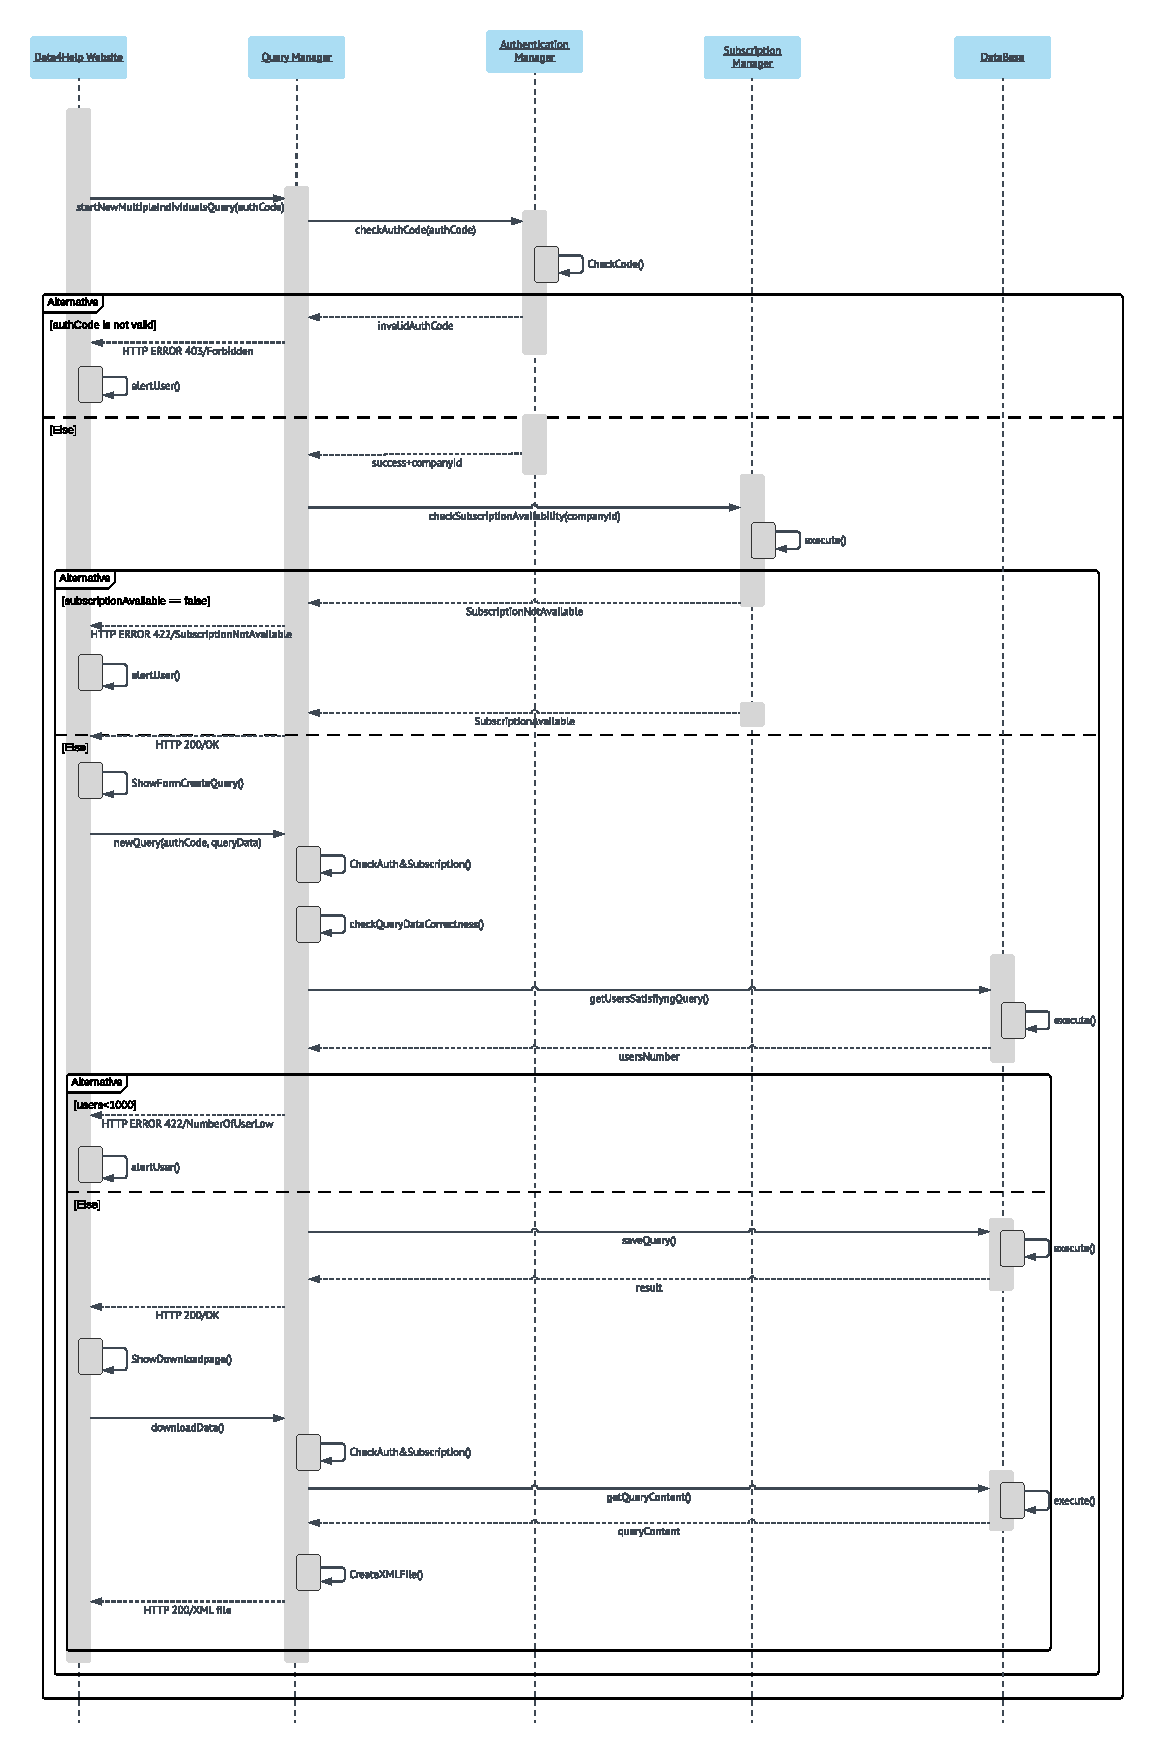
\includegraphics[width=\textwidth,height=\textheight,keepaspectratio]{assets/flowCharts/CompanyQuerySearchMultipleIndividuals.pdf}
	\caption{Company Query Search Multiple Individuals Runtime View}
	\label{fig:CompanyQuerySearchMultipleIndividuals}
\end{figure}

\subsubsection{Company Request Individual Monitoring}
When a Company wants to monitor a single user, it must ask trough the website the permission to the user.\\
The Website sends an HTTP POST request specifiyng the SSN/Fiscal code to monitor to the query manager, that, after checking the correctness of the authToken and obtained the CompanyId, checks with the help of the SubscriptionManager if the company has a plan active that allows it to make this type of query. (omitted from the graph for the sake of readability)\\
If the check passes, a new individual with the state noDecision is inserted in the Database.\\
Then, a notification is sent to the Mobile App instance of the user whose SSN is the object of the query.\\
When the user receives the notification it can either accept it or refuse it. After the click an HTTP POST request is made to the query manager and the query state is updated accordingly.

\begin{figure}[H]
	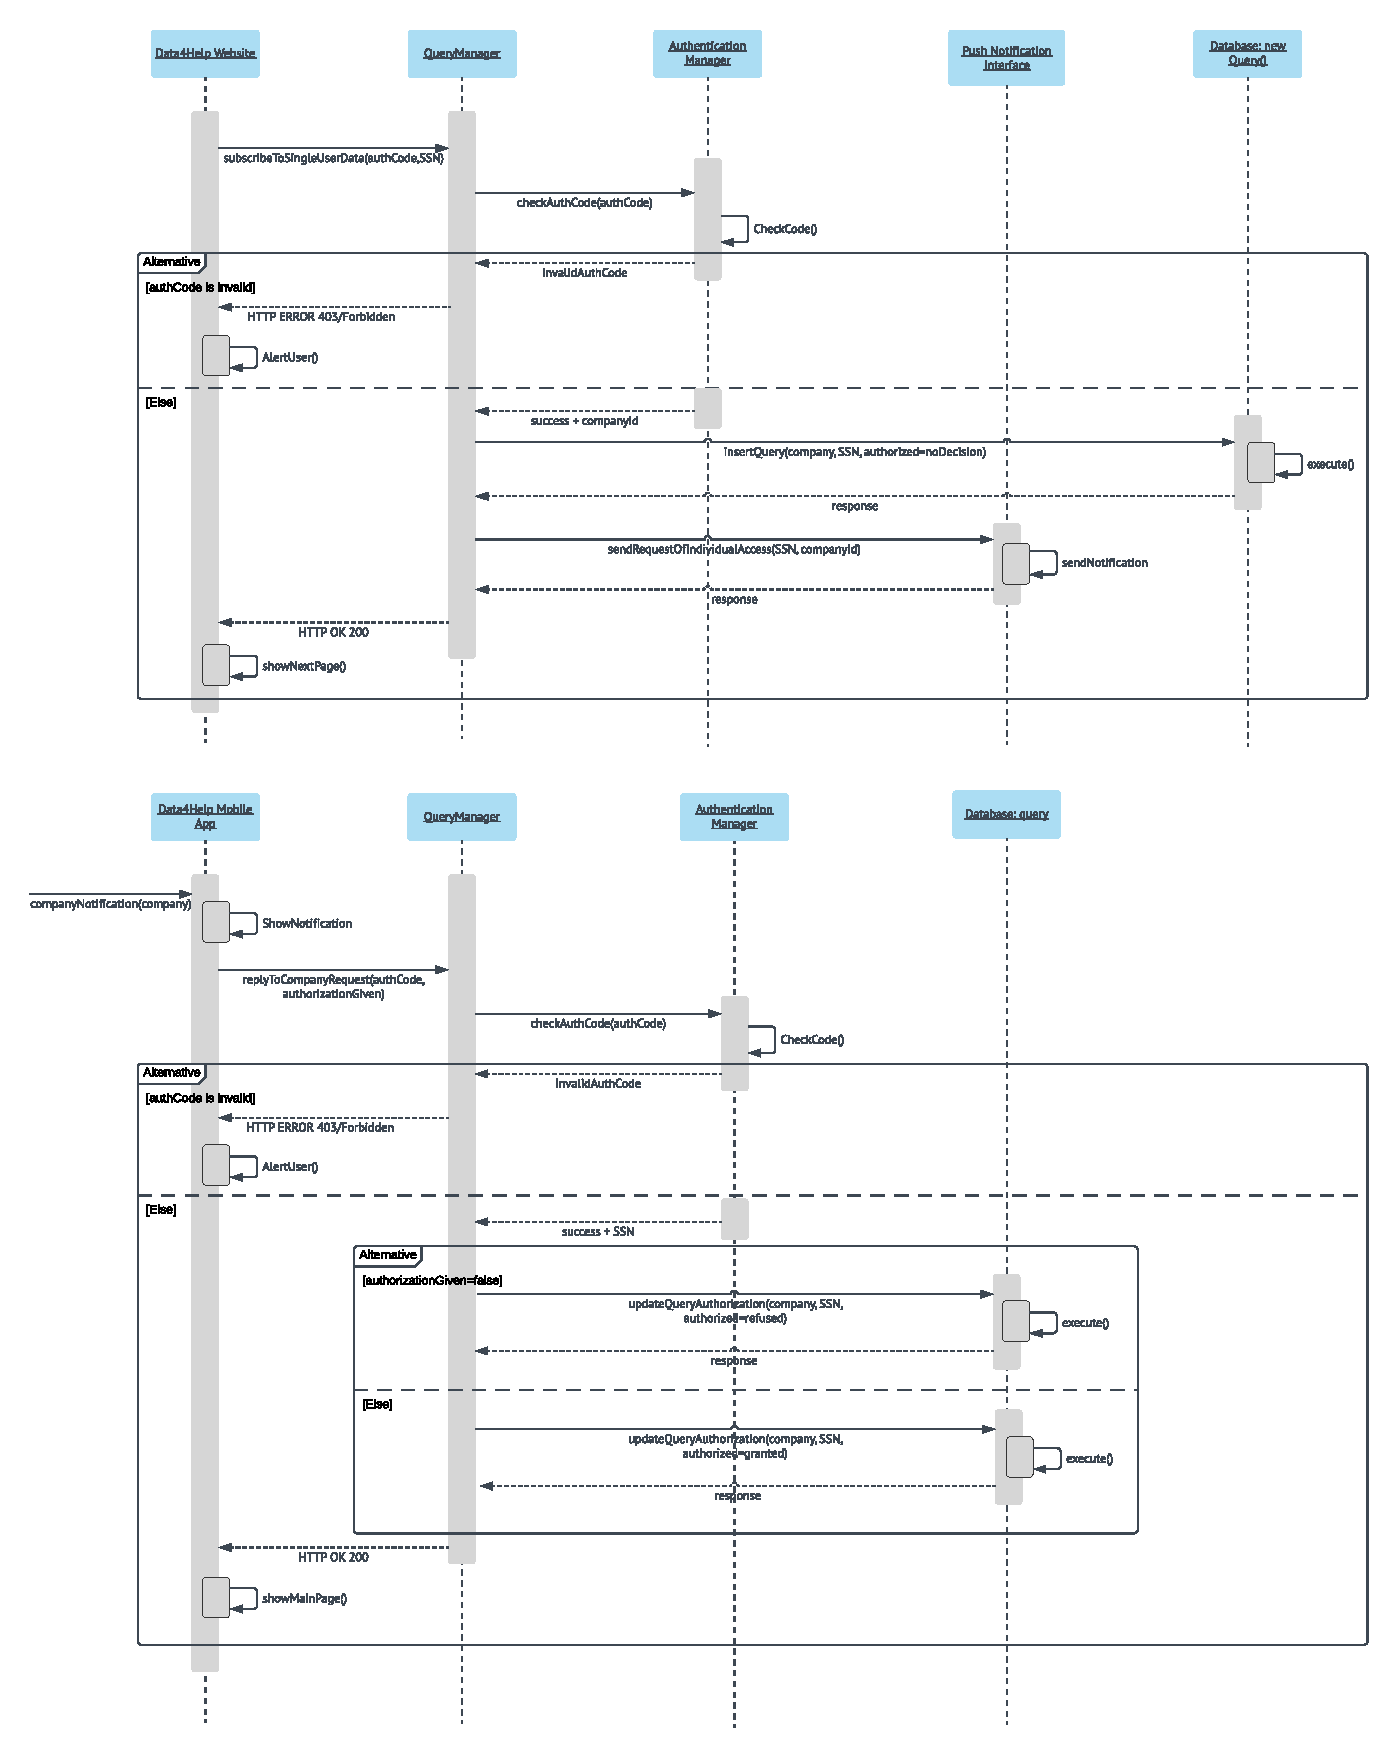
\includegraphics[width=\textwidth,height=\textheight,keepaspectratio]{assets/flowCharts/CompanyRequestIndividualMonitoring.pdf}
	\caption{Company Request Individual Monitoring Runtime View}
	\label{fig:CompanyRequestIndividualMonitoring}
\end{figure}

\subsubsection{Company Consulting Individual}
When a company wants to see an Individual's historical data, through the website, it makes an HTTP GET request to the QueryManager, specifying the SSN, the parameter type and the starting and ending date. The query manager checks the authToken, retrives the companyId and checks if the Company still has a valid plan to make this type of request. If that's indeed the case, the QueryManager checks if the Individual has given Company the authorization to see its data. If this is the case, the user data is retrieved and returned.
\begin{figure}[H]
	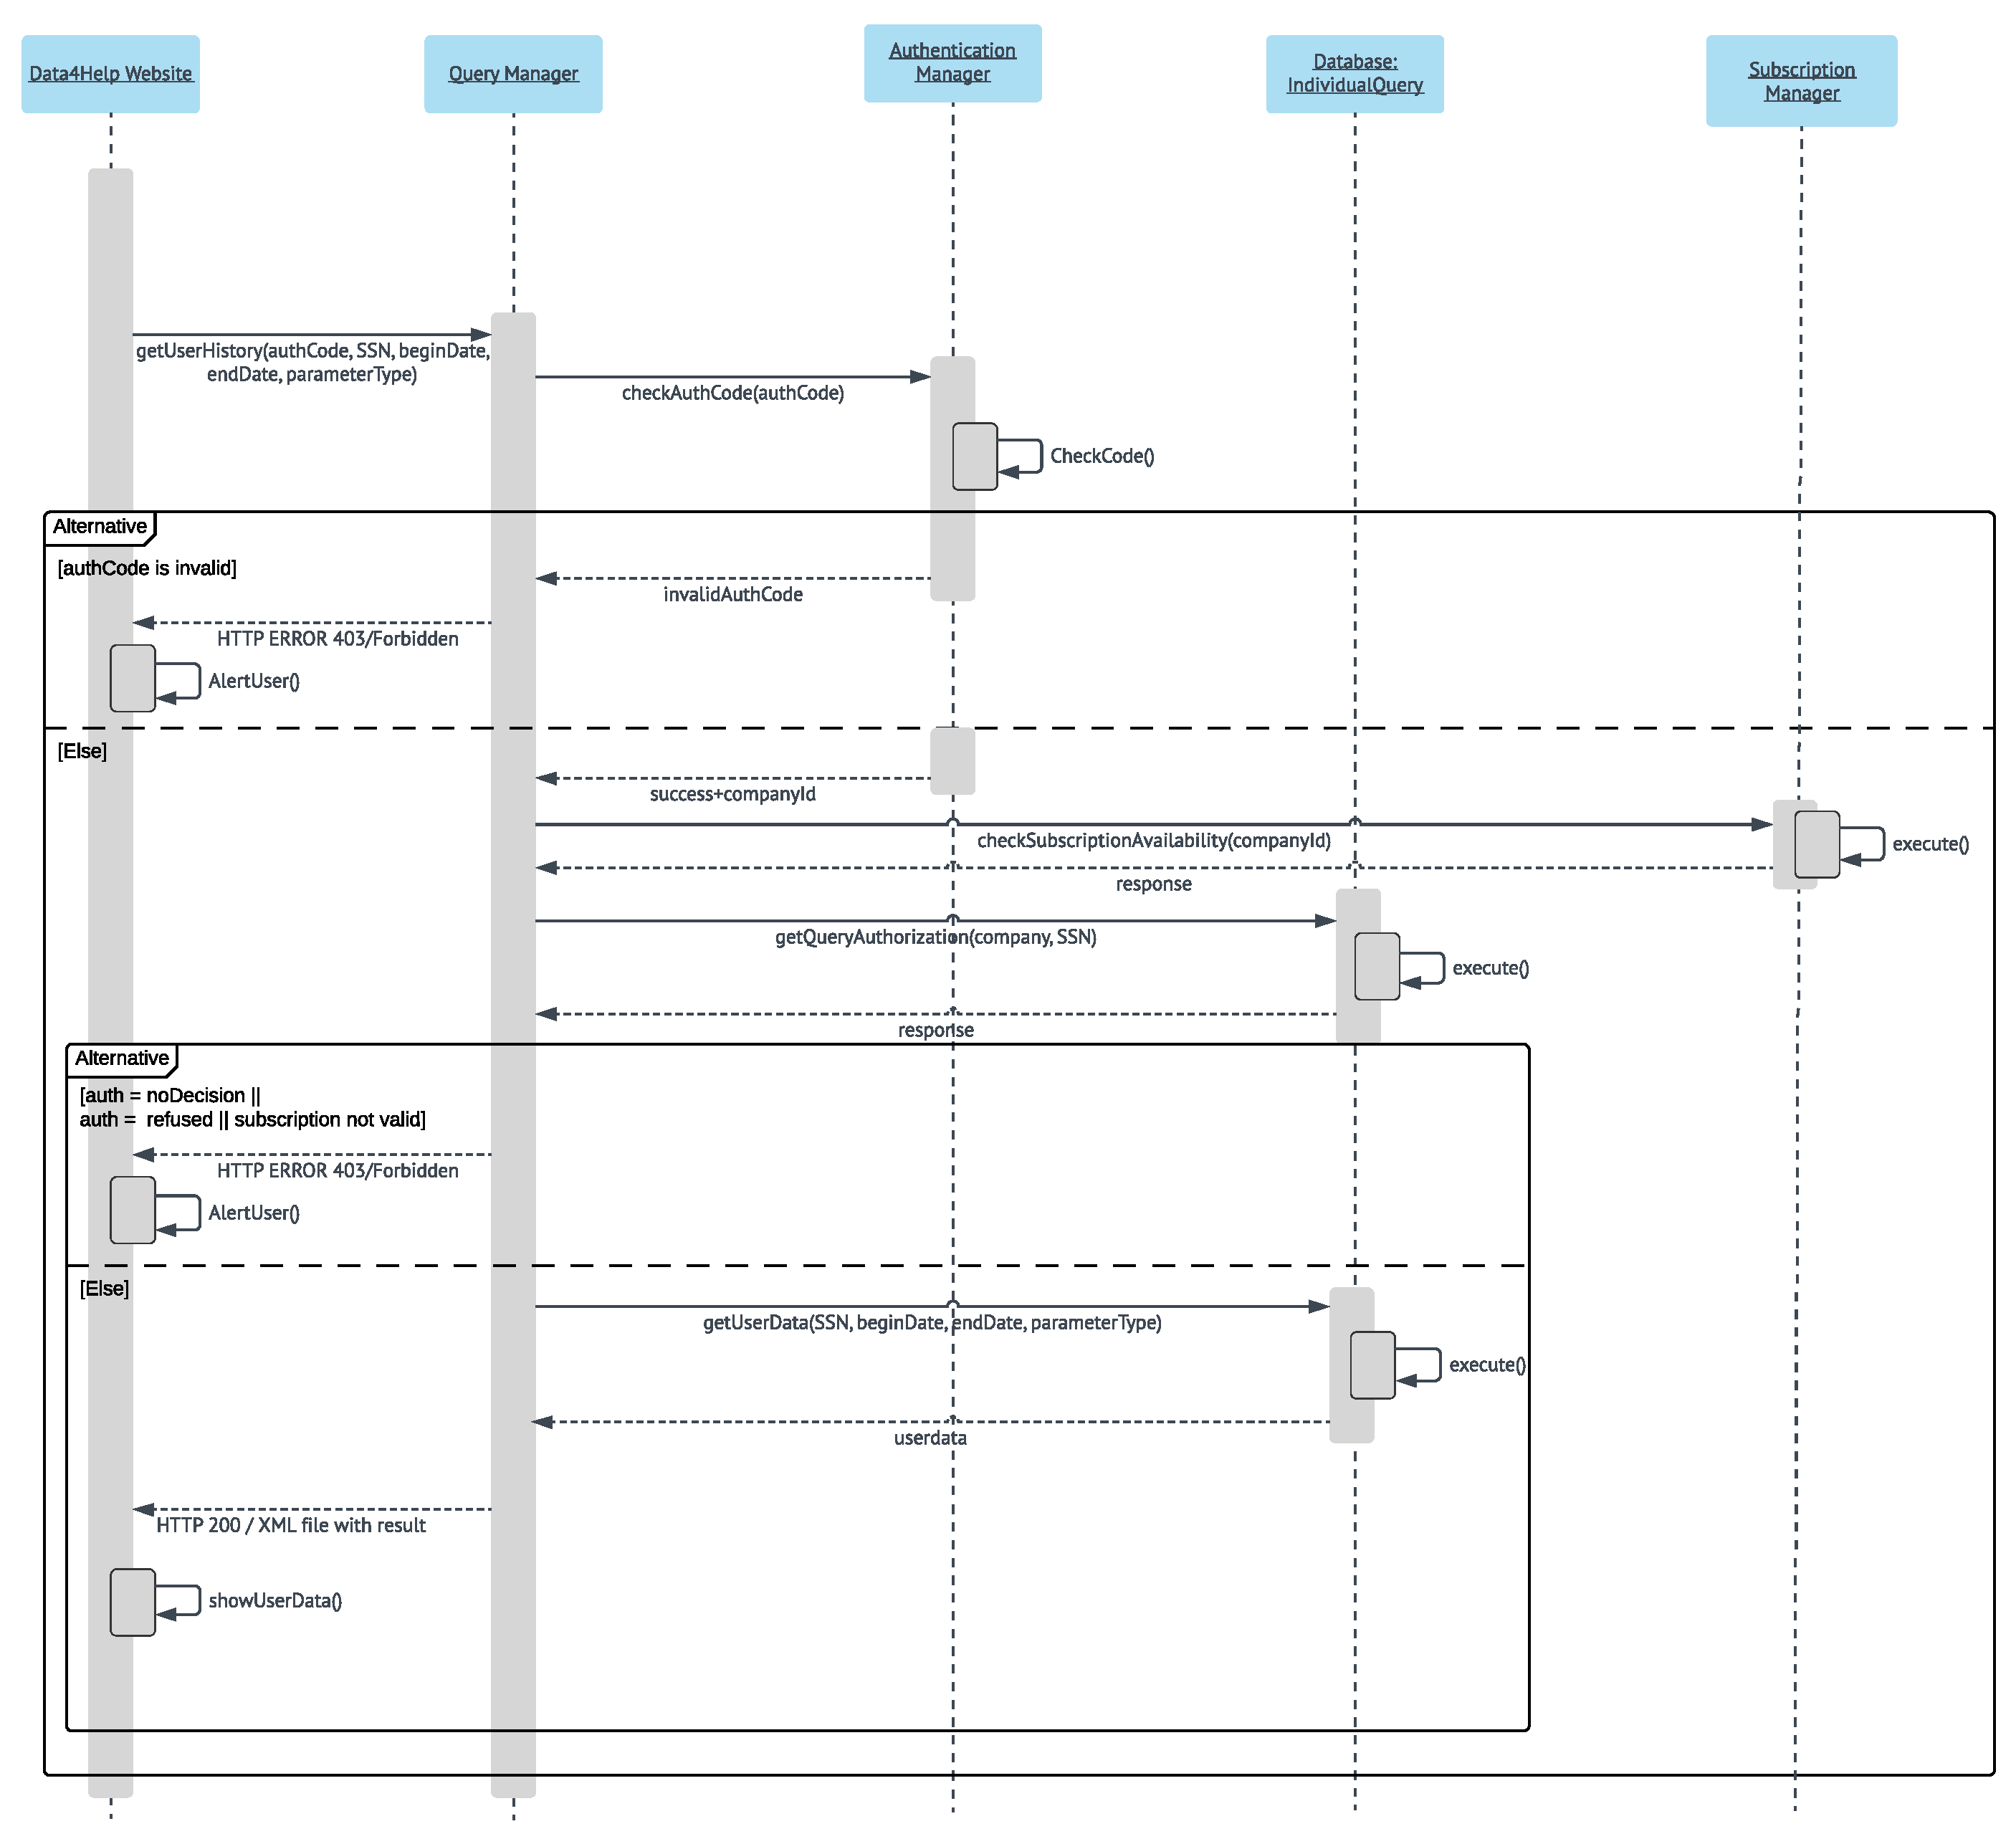
\includegraphics[width=\textwidth,height=\textheight,keepaspectratio]{assets/flowCharts/CompanyConsultingIndividualData.pdf}
	\caption{Company Consulting Individual Data Runtime View}
	\label{fig:CompanyConsultingIndividualData}
\end{figure}

\subsubsection{Company Payment Processing}
When a Company wants to buy a subscription plan, it activates the corresponding functionality in the Website, selects the subscriptionType and insert the credit card number and the CCV/Security code. This data is sent to the server through a HTTP POST request to the SubscriptionManager. After checking the authToken and retrieved the companyId, a call is made to the PaymentInterface to process the payment. If the payment is successfull, the subscription is inserted in the Database and linked to the company.
\begin{figure}[H]
	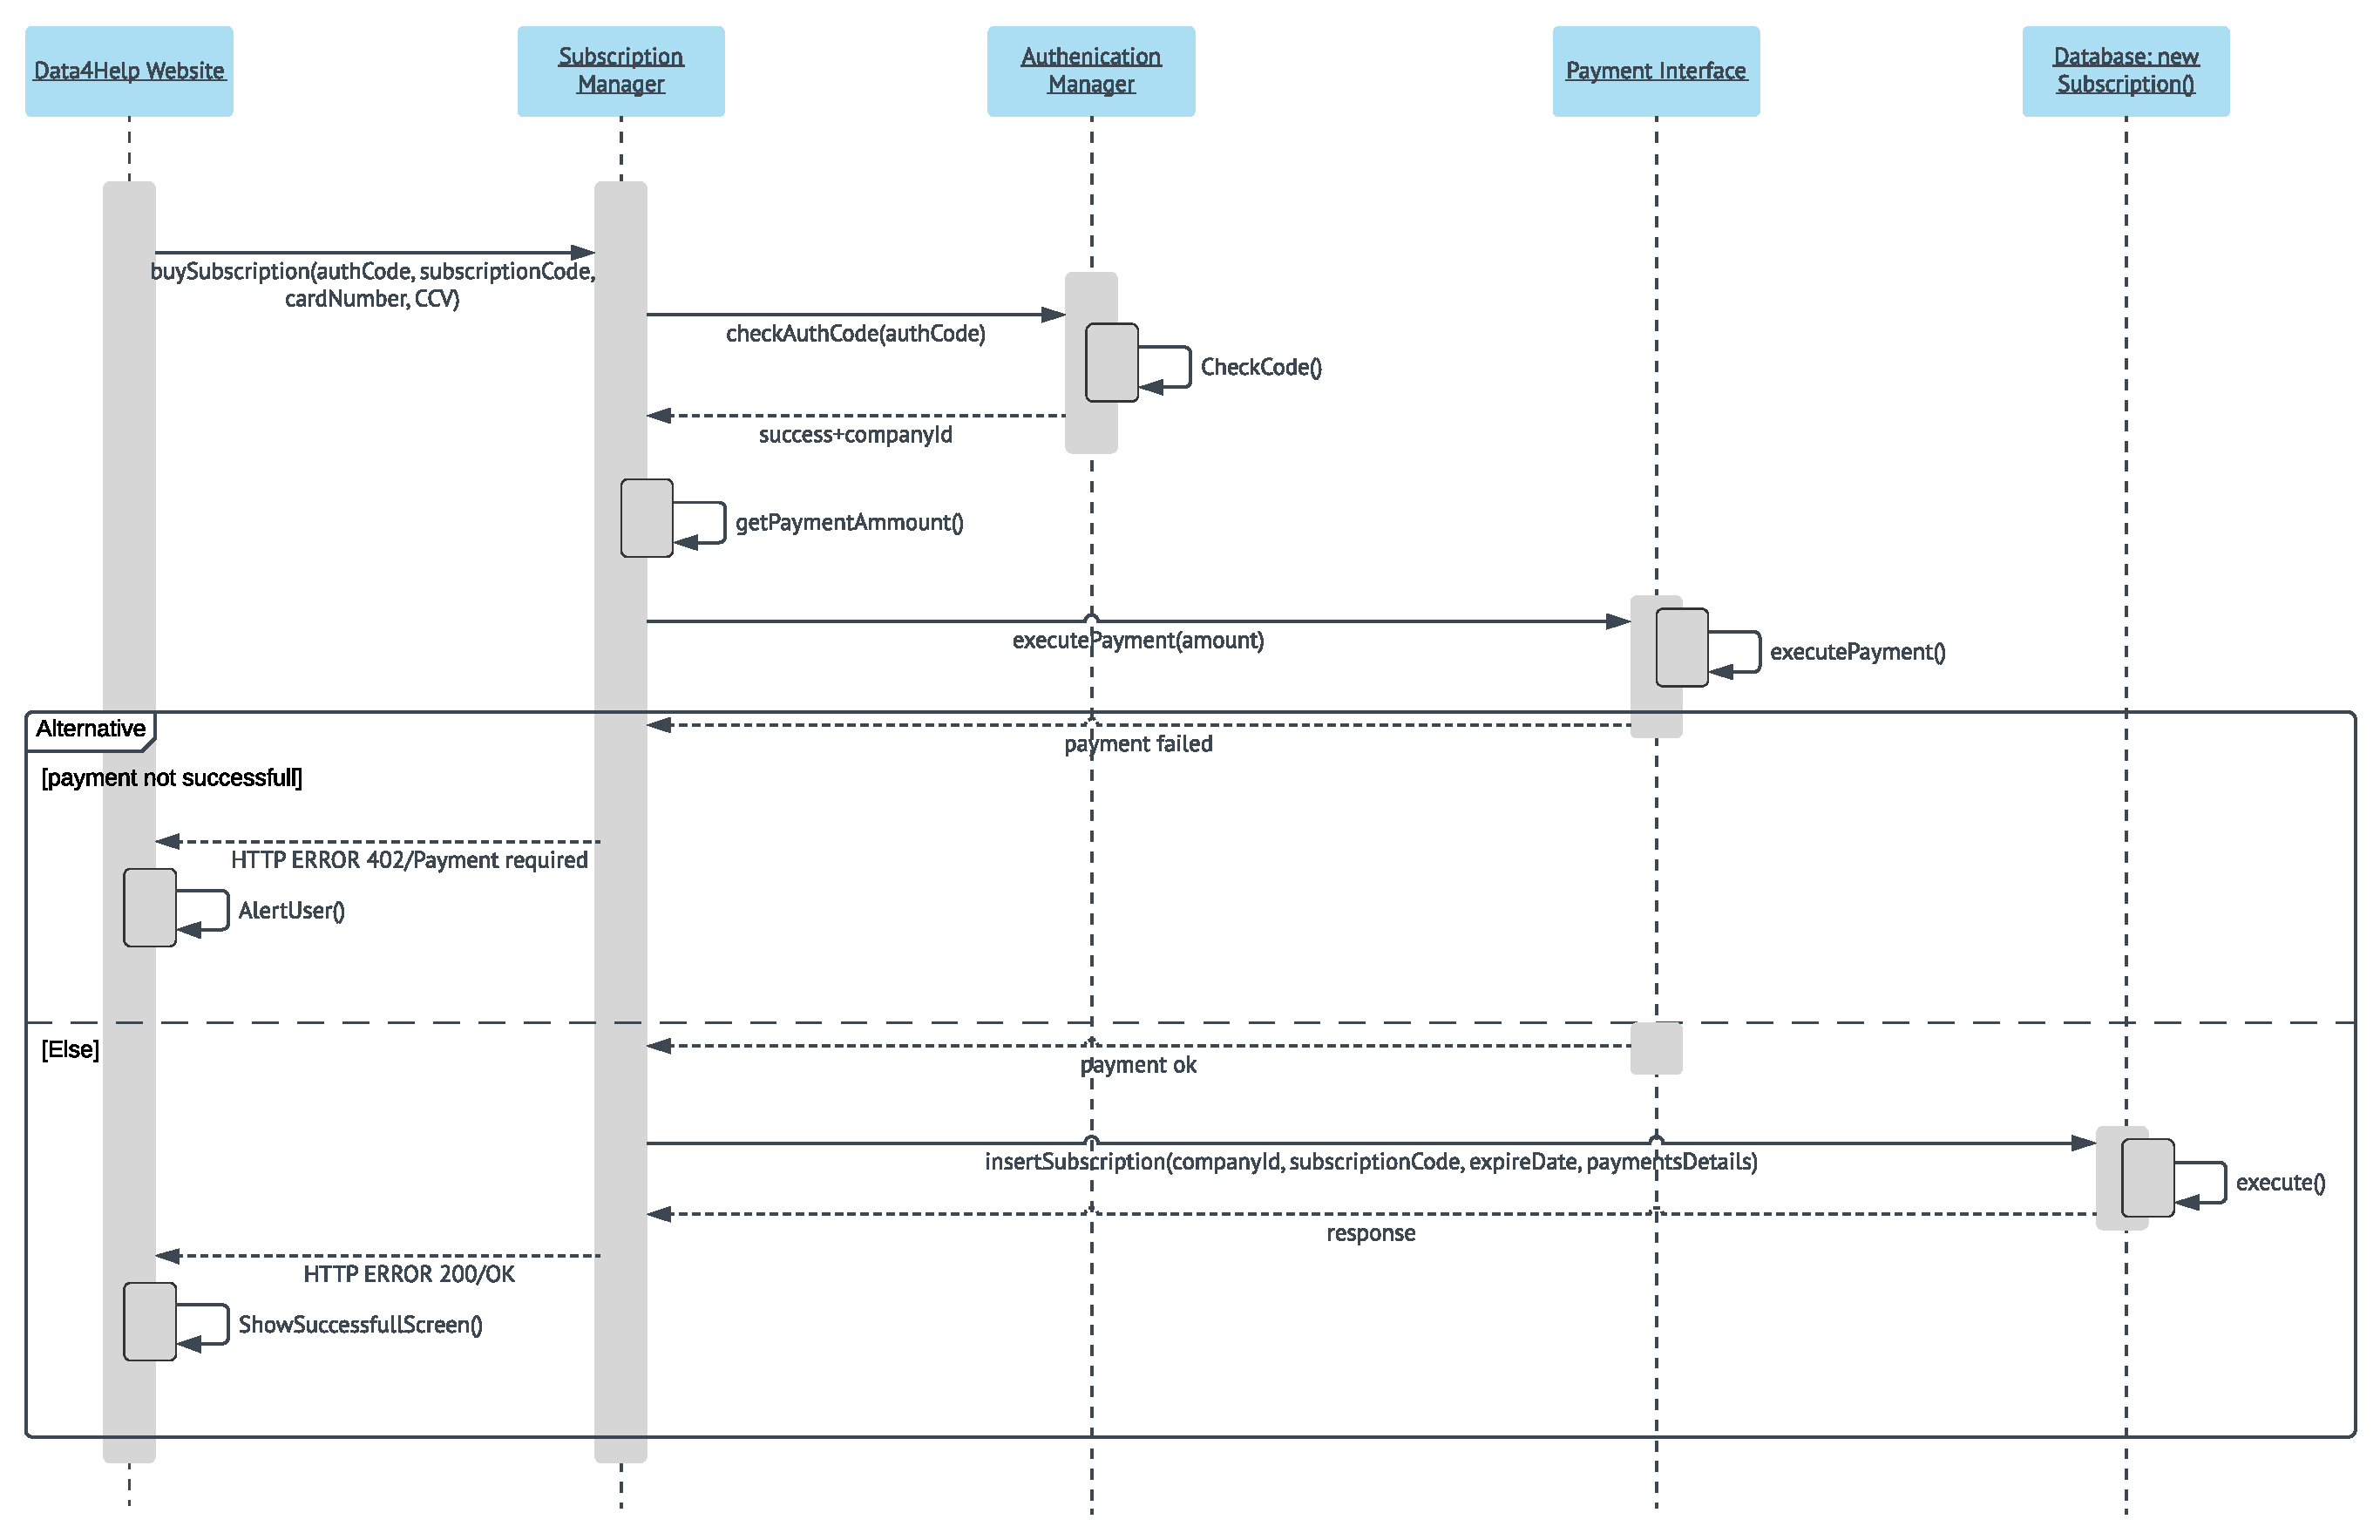
\includegraphics[width=\textwidth,height=\textheight,keepaspectratio]{assets/flowCharts/CompanyPaymentProcessing.pdf}
	\caption{Company Payment Processing Runtime View}
	\label{fig:CompanyPaymentProcessing}
\end{figure}


\subsubsection{Emergency Situation}
If a user is subscribed to the AutomatedSOS service, whenever the Individual Manager receives new data from the Mobile App, it also sends a checkUserThresholds request to the EmergencyManager, specifying the SSN of the individual and the health data received. Firstly the EmergencyManager checks if the user is subscribed to AutomatedSOS, if so, it checks the threshold for that specific user: in the case in which the data parameters are lower than the specified threshold, the EmergencyManager instantly sends a sendAmbulance request to the EmergencyInterface, which will contact the ambulance API and requests an ambulance for the person. To do so, in the request includes the user position. 
\begin{figure}[H]
	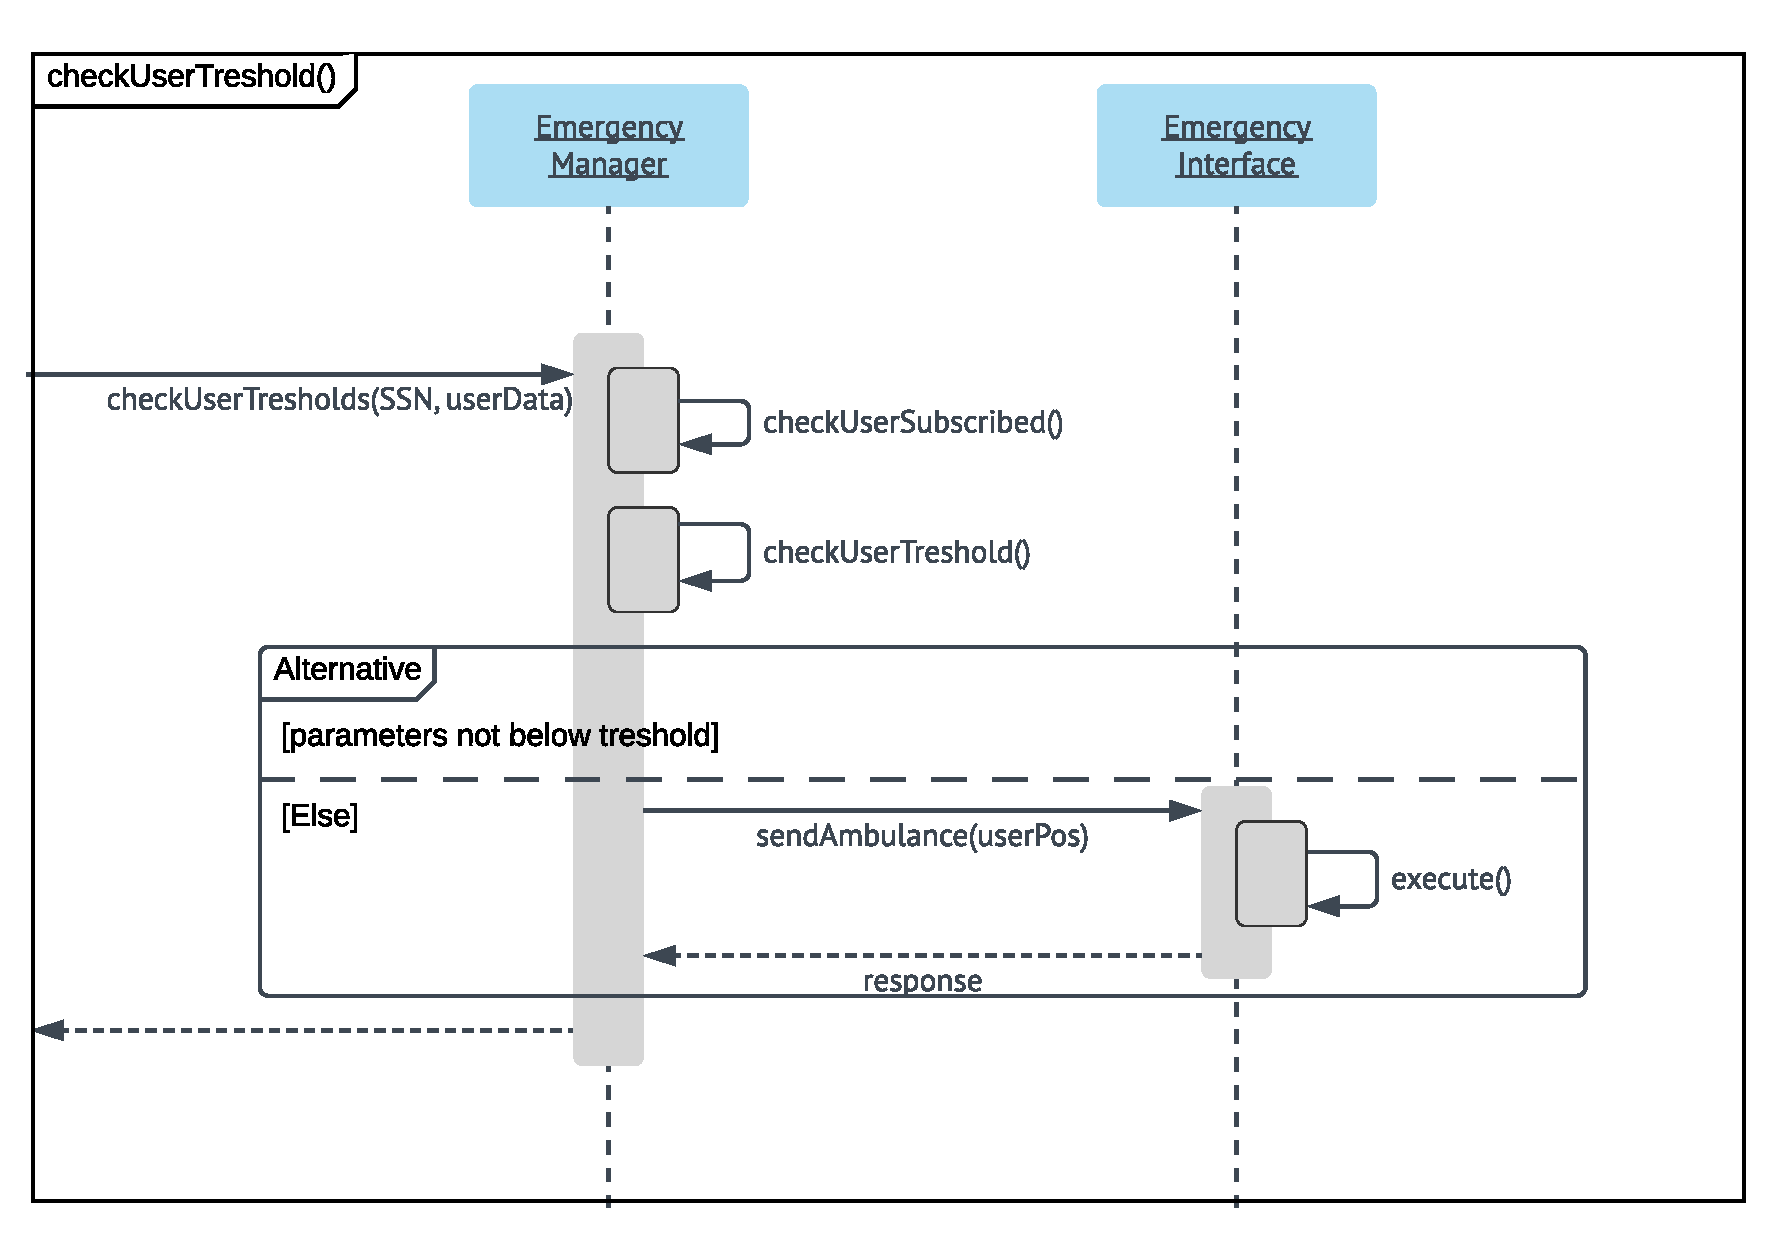
\includegraphics[width=\textwidth,height=\textheight,keepaspectratio]{assets/flowCharts/EmergencySituation.pdf}
	\caption{Emergency Situation Runtime View}
	\label{fig:EmergencySituation}
\end{figure}


\subsubsection{Run Organizer Adds New Race}
When a run organizer wants to add a new race using the Data4Help Mobile App, he goes to the corresponding section, fills information about the run and clicks on "Create new run".\\
The website sends a createNewRun request specifying the authToken and runData, the Authentication manager authenticates the user, and checks data consistency.
If data is consistent, the Run Manager goes on inserting the new run into the Track4Me database and returns a successfull response to the client, otherwise it returns an error and alerts the user.
\begin{figure}[H]
	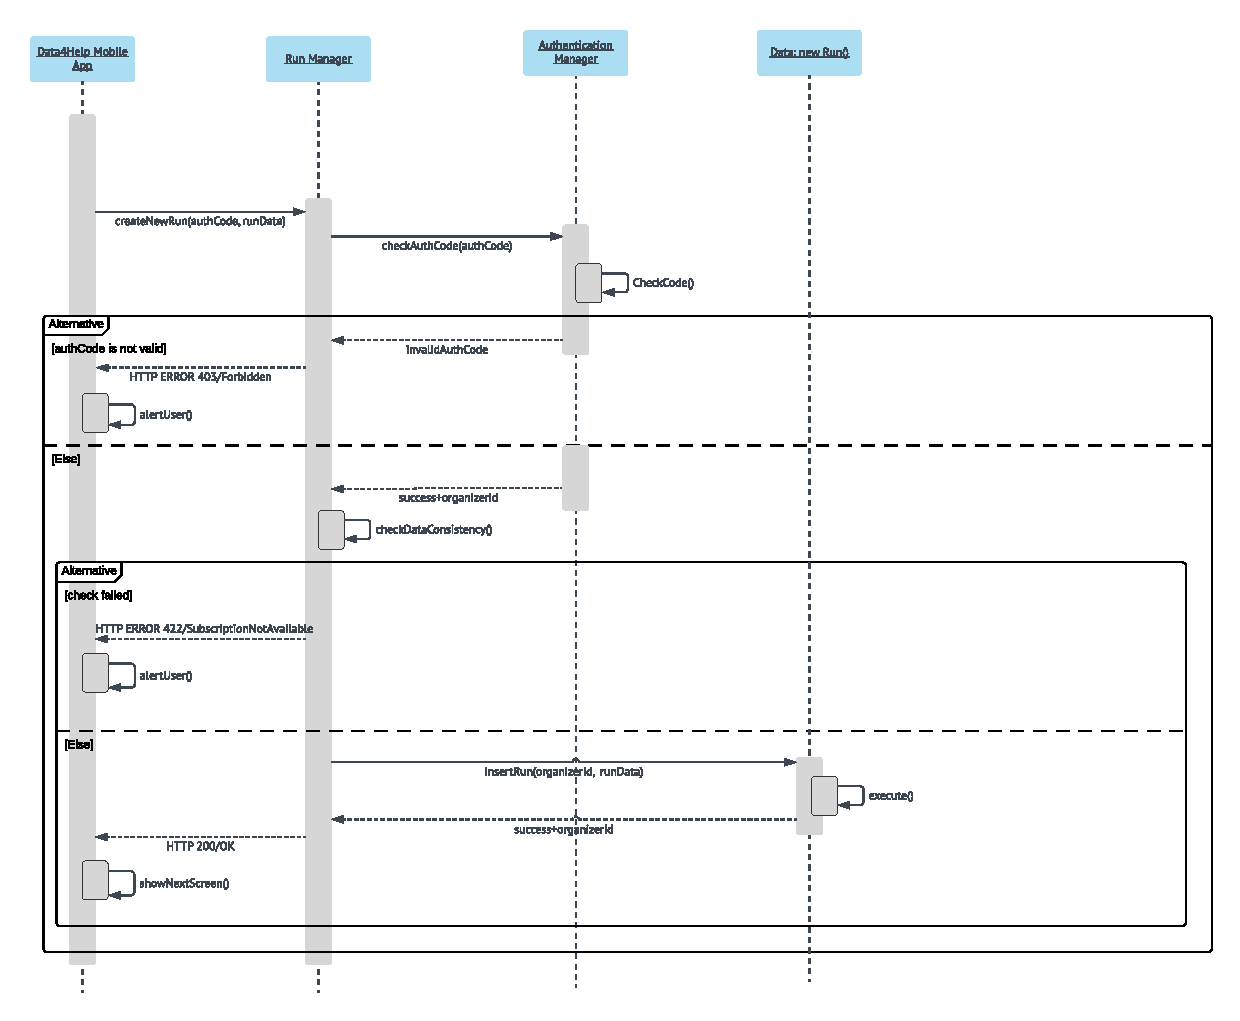
\includegraphics[width=\textwidth,height=\textheight,keepaspectratio]{assets/flowCharts/RunOrganizerAddsNewRace.pdf}
	\caption{Run Organizer Adds New Race Runtime View}
	\label{fig:RunOrganizerAddsNewRace}
\end{figure}



\subsubsection{Runner Subscription To A Race}
When a user of Data4Help wants to subscribe to a run, it must send a getRunList request containing its geographical position to the RunManager. \\
Firstly, the RunManager computes which races have their starting point 30km close to the runner position, then returns the mentioned list to the user. 
Then, the user chooses the run he wants to subscribe to and sends a subscribeUser request to the RunManager containing the authToken and the runId. \\
The user is authenticated by the Authentication Manager, if the sent authToken is correct, the RunManager goes on checking if the chosen race has already started.\\ If the race has already started, the Run Manager sends an error to the client, otherwise, adds the user to the runner lists sending an addUserToRun to the Run Manager(specifying the user SSN and the runId).\\

\begin{figure}[H]
	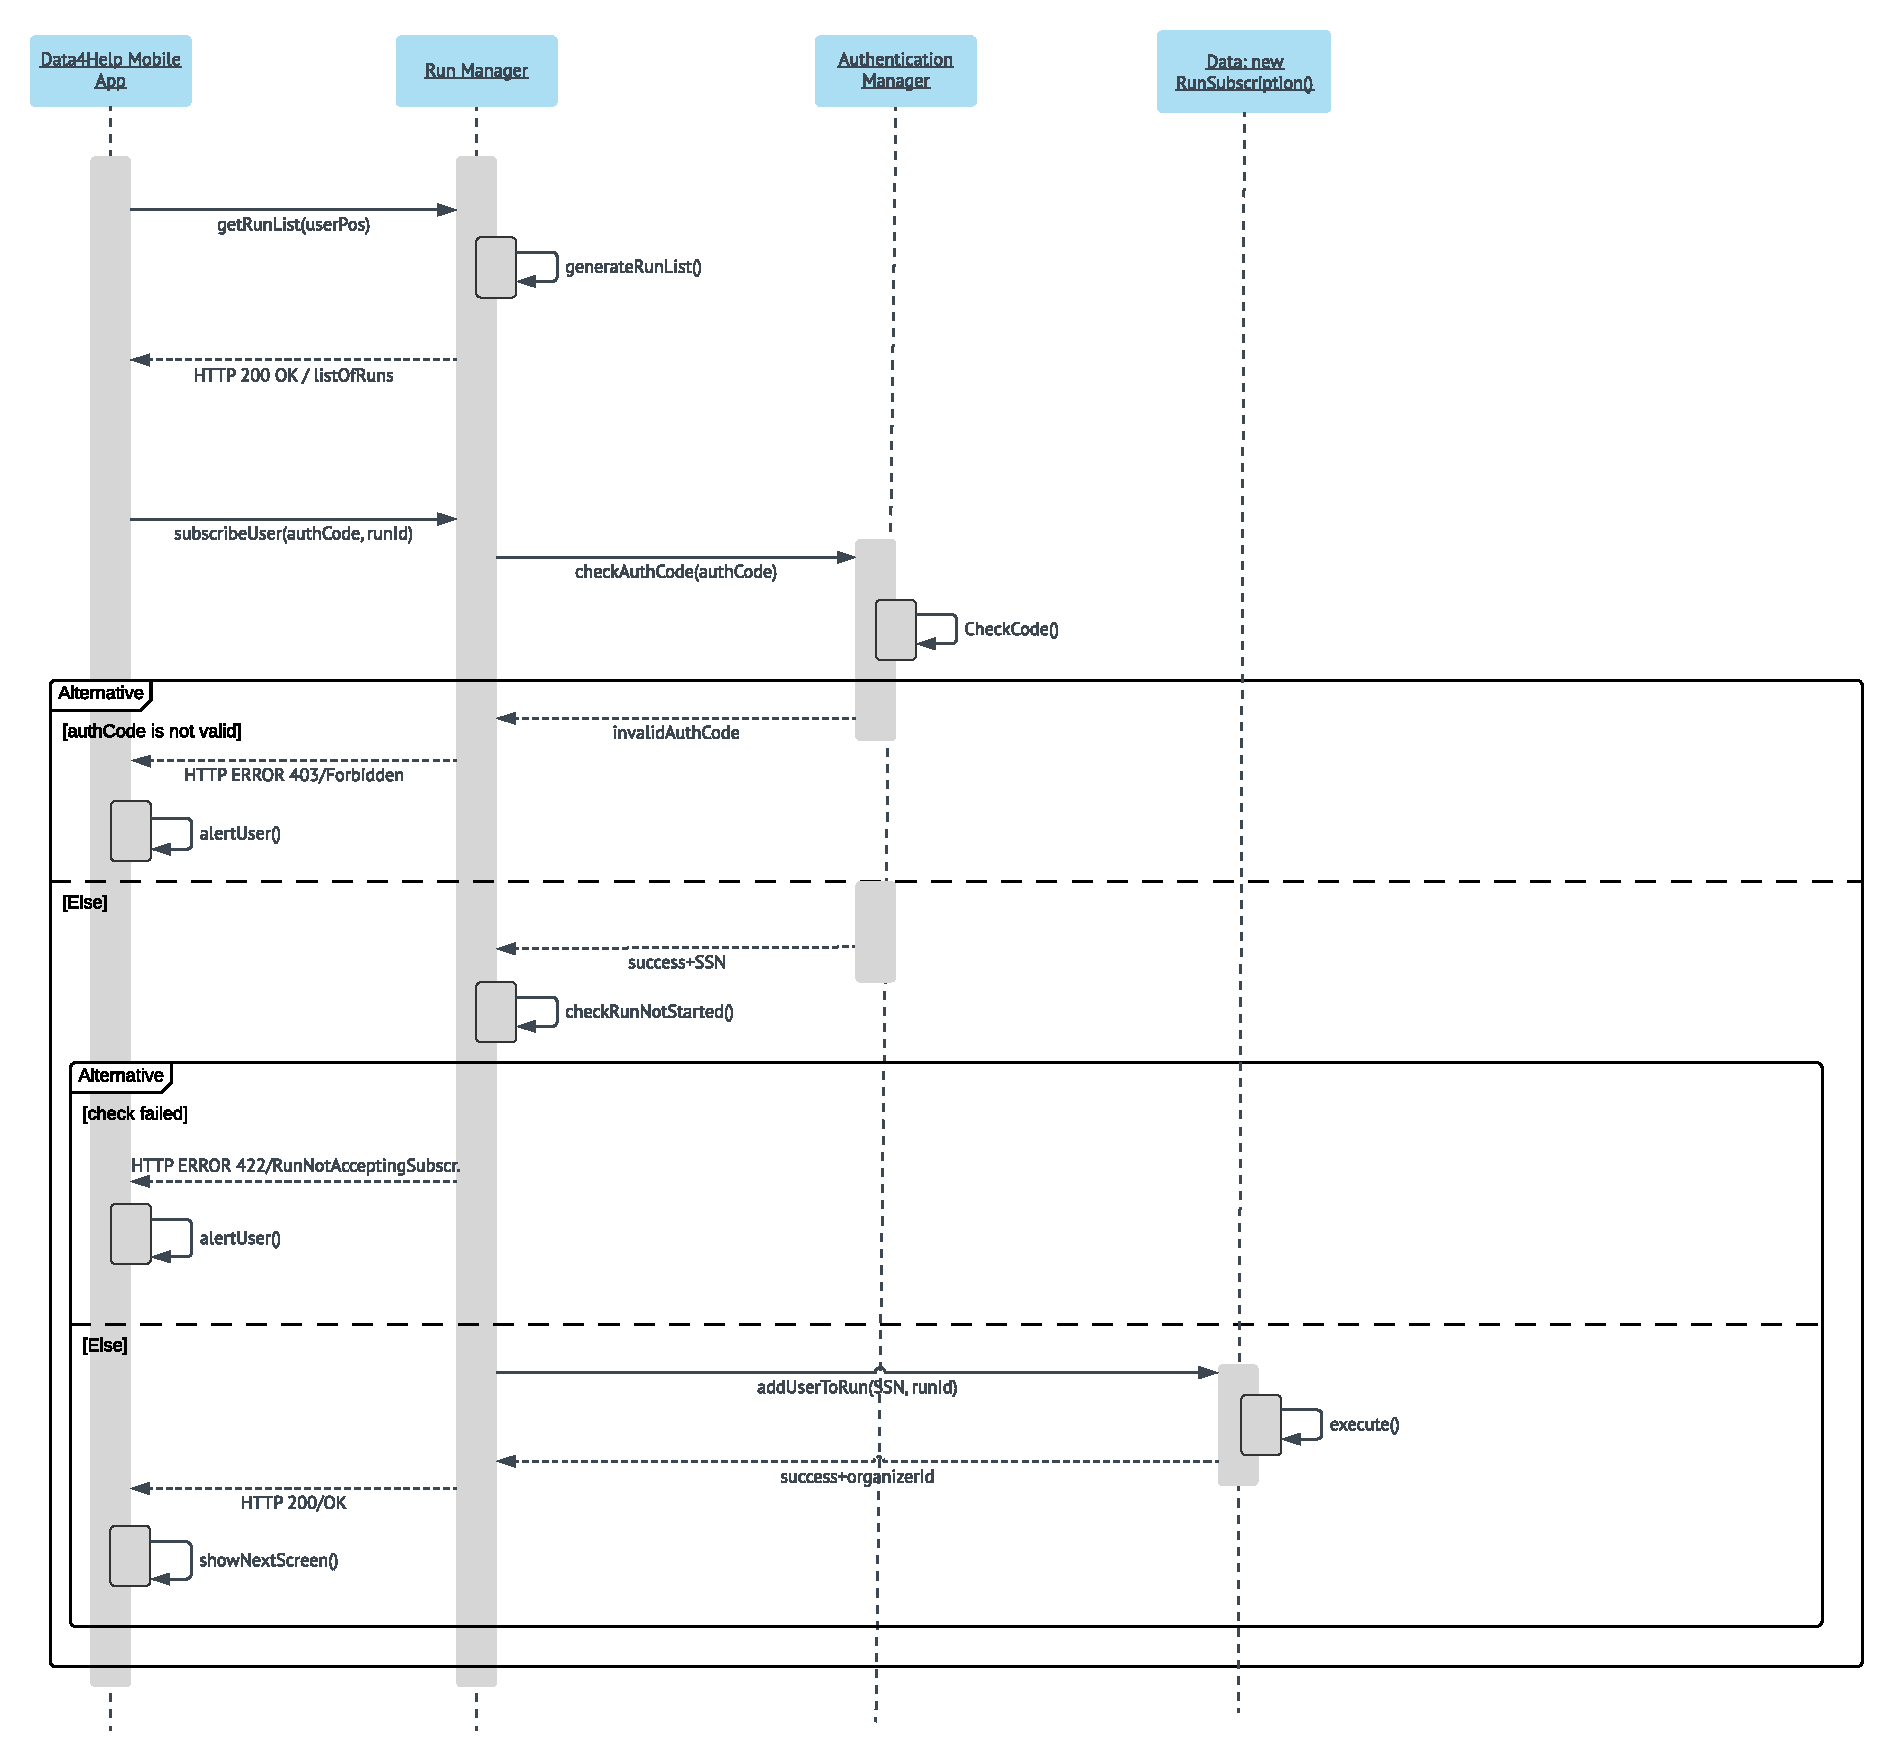
\includegraphics[width=\textwidth,height=\textheight,keepaspectratio]{assets/flowCharts/RunnerSubscriptionToARace.pdf}
	\caption{Runner Subscription To A Race Runtime View}
	\label{fig:RunnerSubscriptionToARace}
\end{figure}


\subsubsection{Spectator Of Run Request Run Position}
When a user wants to see the map of the runners of a run, he must request the runner positions to the RunManager.\\
The Mobile app sends an getRunnerPositions request specifiyng the code of the run followed to the RunManager that, after checking if the run is still active, get all the users position in run identifying them with the SSN.\\ Then, it sends a getUserPosFromDatetime request, specifying the runStartDatetime, it computes if the user has passed checkpoints (computeCheckPoint), eventually add the information of the user in a list. \\
Finally, the userList with the data about checkpoint passed and the geographical position is returned to the Mobile App, that shows in a map all runner positions.


\begin{figure}[H]
	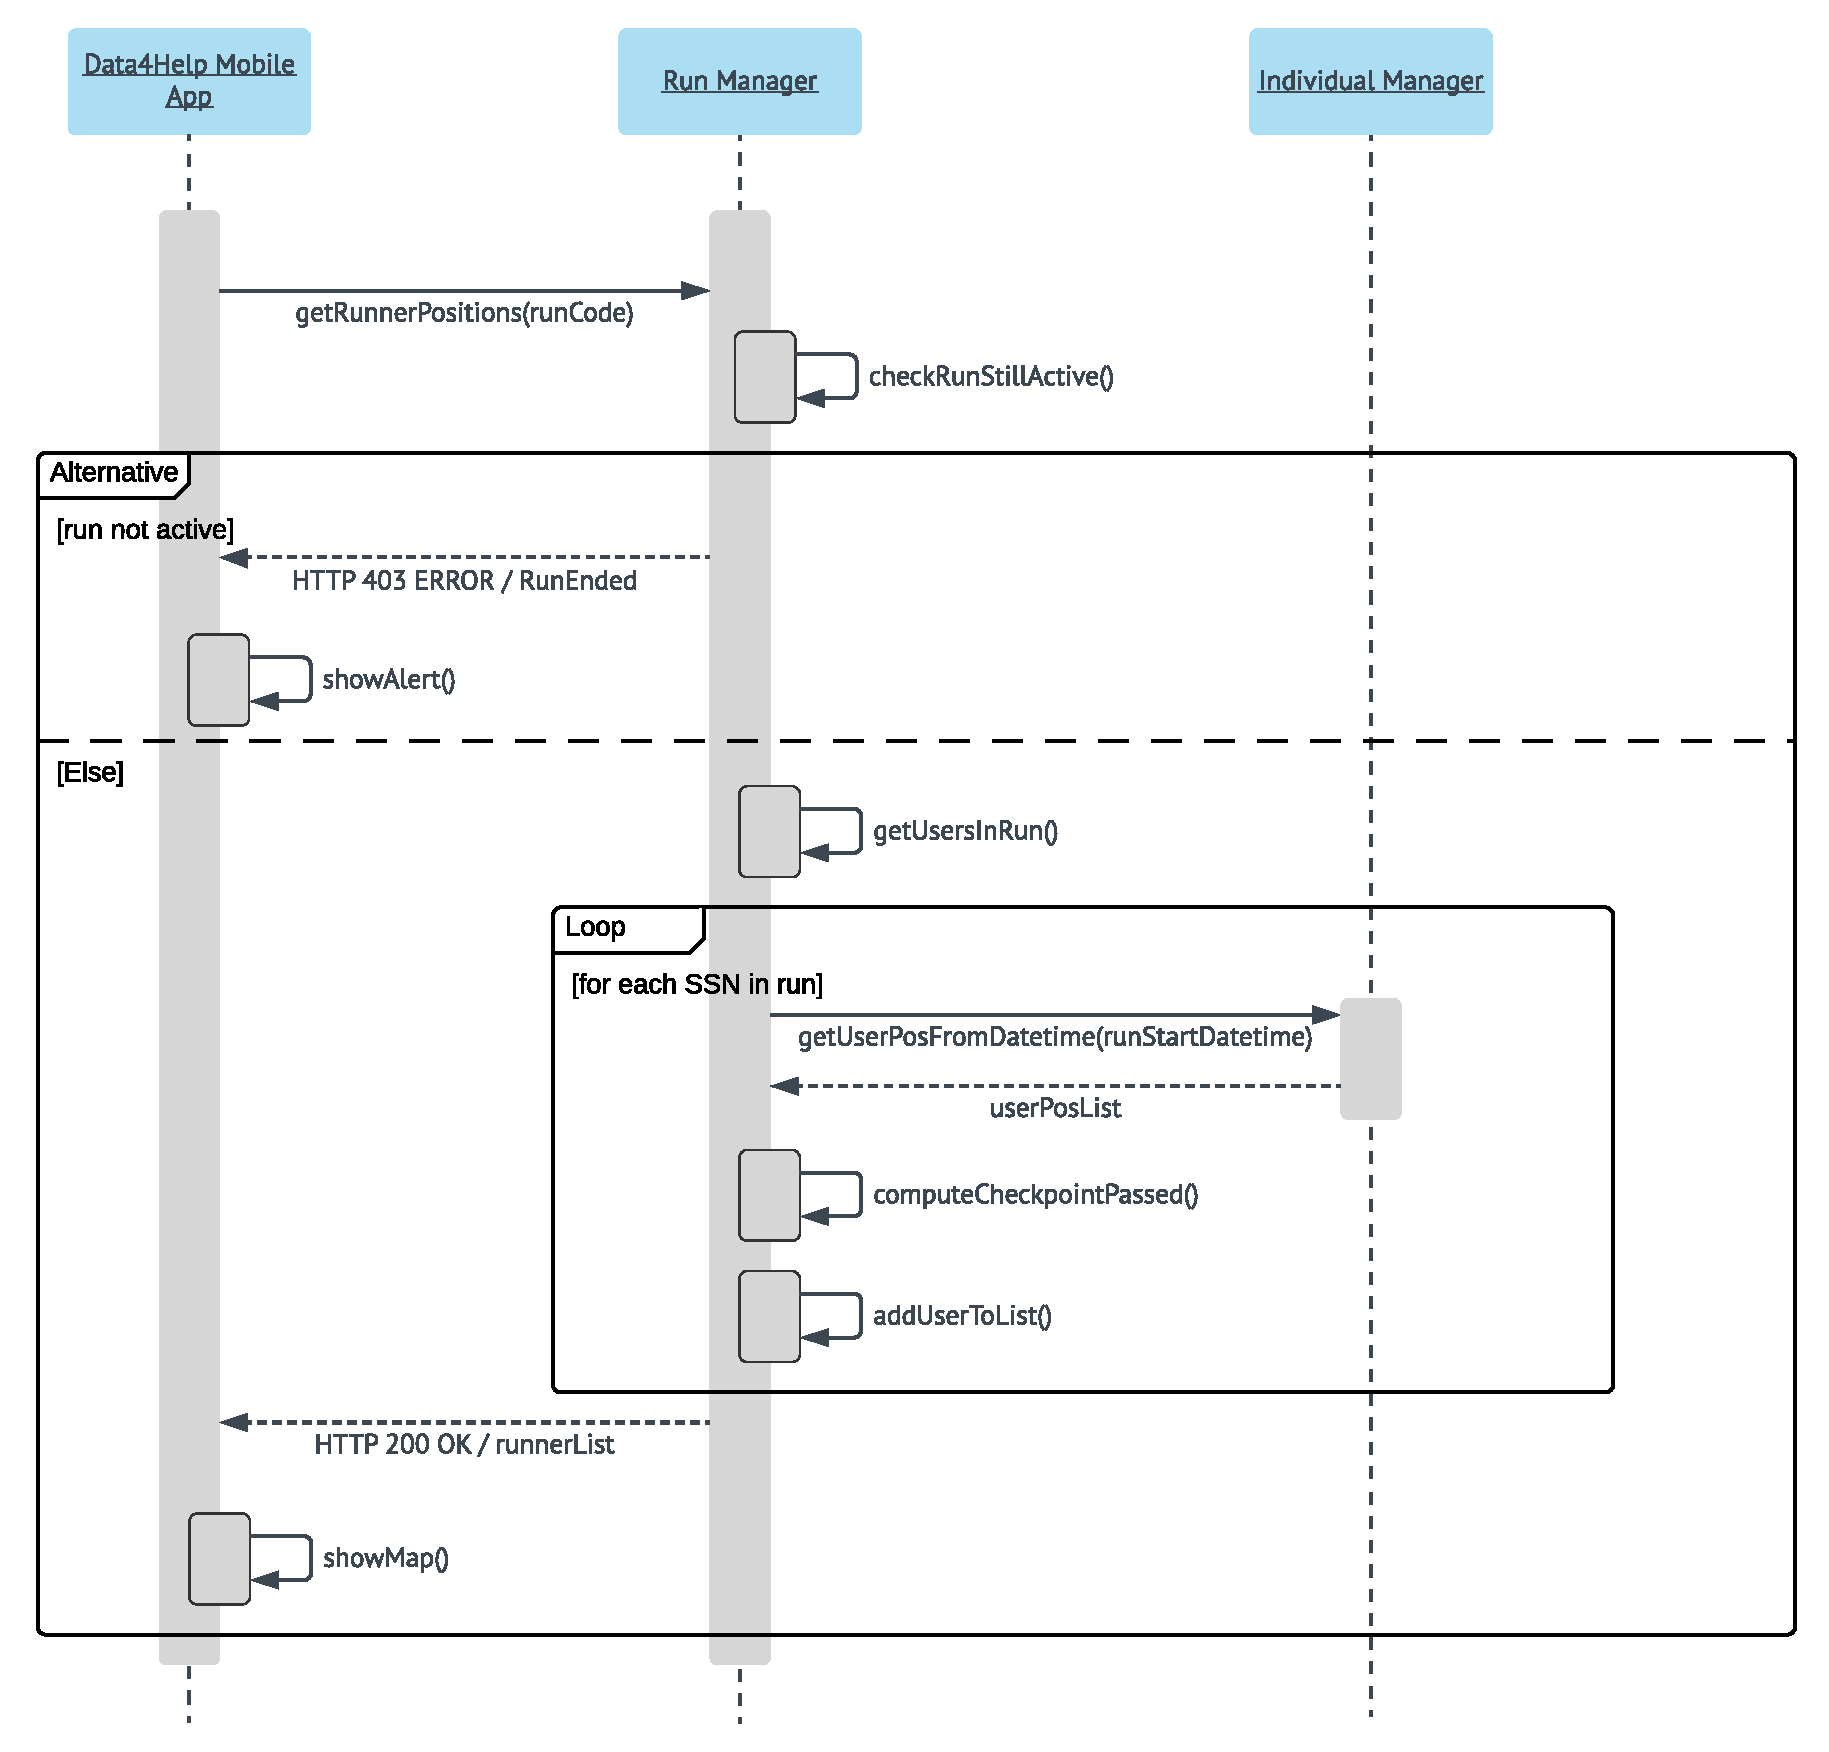
\includegraphics[width=\textwidth,height=\textheight,keepaspectratio]{assets/flowCharts/SpectatorOfRunRequestRunPosition.pdf}
	\caption{Spectator Of Run Request Run Position Runtime View}
	\label{fig:SpectatorOfRunRequestRunPosition}
\end{figure}
        \subsection{Component interfaces}
            \subsubsection{REST API}
    \textbf{Authentication Manager}
    \begin{itemize}
        \item User Registration
    \end{itemize}
    \begin{adjustwidth}{1cm}{}
        \begin{longtable}{|c|l|}
            \hline
            \textbf{Endpoint} & /auth/register\_user \\
            \hline
            \textbf{URL Params} &  \\
            \hline
            \textbf{Method} & \textbf{POST} \\
            \hline
            \textbf{Request Data} & mail: String \\
            &                 password: String \\
            &                 SSN: String \\
            &                 name: String \\
            &                 surname: String \\
            &                 birthday: Date \\
            &                 smartwatch: String \\
            \hline
            \textbf{Success Response} & code: \texttt{200 OK} \\
            &                           content: \\
            & \begin{minipage}[t]{0.5\textwidth}
                \begin{adjustwidth}{1.5cm}{}
                \begin{verbatim}
{
    success: true, 
    auth_code: ...
}
                \end{verbatim}
                \end{adjustwidth}
              \end{minipage} \\
              \hline
            \textbf{Error Response} & code: \texttt{422 UNPROCESSABLE ENTITY} \\
            &                         content: \\
            & \begin{minipage}[t]{0.7\textwidth}
                \begin{adjustwidth}{1.5cm}{}
                \begin{verbatim}
{
    success: false, 
    error: 'InfoNotValid',
    message: ...
}
                \end{verbatim}
                \end{adjustwidth}
                \texttt{message} can be one of the following: 
                \begin{itemize}
                    \item \texttt{Unsupported smartwatch}
                    \item \texttt{Mail already used}
                    \item \texttt{SSN not valid}
                \end{itemize}
              \end{minipage} \\
              \hline
            \textbf{Uses} & Allows the client to register a new User \\
            \hline
        \end{longtable}
    \end{adjustwidth}

    \begin{itemize}
        \item Company Registration
    \end{itemize}
    \begin{adjustwidth}{1cm}{}
        \begin{longtable}{|c|l|}
            \hline
            \textbf{Endpoint} & /auth/register\_company \\
            \hline
            \textbf{URL Params} &  \\
            \hline
            \textbf{Method} & \textbf{POST} \\
            \hline
            \textbf{Request Data} & email: String \\
            &                 password: String \\
            &                 company\_name: String \\

            \hline
            \textbf{Success Response} & code: \texttt{200 OK} \\
            &                           content: \\
            & \begin{minipage}[t]{0.5\textwidth}
                \begin{adjustwidth}{1.5cm}{}
                \begin{verbatim}
{
    success: true, 
    auth_code: ...
}
                \end{verbatim}
                \end{adjustwidth}
              \end{minipage} \\
              \hline
            \textbf{Error Response} & code: \texttt{422 UNPROCESSABLE ENTITY} \\
            &                         content: \\
            & \begin{minipage}[t]{0.7\textwidth}
                \begin{adjustwidth}{1.5cm}{}
                \begin{verbatim}
{
    success: false, 
    error: 'InfoNotValid',
    message: ...
}
                \end{verbatim}
                \end{adjustwidth}
                \texttt{message} can be one of the following: 
                \begin{itemize}
                    \item \texttt{Email already in use}
                \end{itemize}
              \end{minipage} \\
              \hline
            \textbf{Uses} & Allows the client to register a new Company \\
            \hline
        \end{longtable}
    \end{adjustwidth}

\begin{itemize}
        \item Run Organizer Registration
    \end{itemize}
    \begin{adjustwidth}{1cm}{}
        \begin{longtable}{|c|l|}
            \hline
            \textbf{Endpoint} & /auth/register\_run\_organizer \\
            \hline
            \textbf{Method} & \textbf{POST} \\
            \hline
            \textbf{URL Params} &  \\
            \hline
            \textbf{Request Data} & email: String \\
            &                 password: String \\
            &                 name: String \\
            &                 surname: String \\
            \hline
            \textbf{Success Response} & code: \texttt{200 OK} \\
            &                           content: \\
            & \begin{minipage}[t]{0.5\textwidth}
                \begin{adjustwidth}{1.5cm}{}
                \begin{verbatim}
{
    success: true, 
    auth_code: ...
}
                \end{verbatim}
                \end{adjustwidth}
              \end{minipage} \\
              \hline
            \textbf{Error Response} & code: \texttt{422 UNPROCESSABLE ENTITY} \\
            &                         content: \\
            & \begin{minipage}[t]{0.7\textwidth}
                \begin{adjustwidth}{1.5cm}{}
                \begin{verbatim}
{
    success: false, 
    error: 'InfoNotValid',
    message: ...
}
                \end{verbatim}
                \end{adjustwidth}
                \texttt{message} can be one of the following: 
                \begin{itemize}
                    \item \texttt{SSN not valid}
                \end{itemize}
              \end{minipage} \\
              \hline
            \textbf{Uses} & Allows the client to register a new run organizer \\
            \hline
        \end{longtable}
    \end{adjustwidth}

    \begin{itemize}
        \item User Login
    \end{itemize}
    \begin{adjustwidth}{1cm}{}
        \begin{longtable}{|c|l|}
            \hline
            \textbf{Endpoint} & /auth/login \\
            \hline
            \textbf{Method} & \textbf{POST} \\
            \hline
            \textbf{URL Params} &  \\
            \hline
            \textbf{Request Data} & email: String \\
            &                 password: String \\
            &                 type: String \\
            \hline
            \textbf{Success Response} & code: \texttt{200 OK} \\
            &                           content: \\
            & \begin{minipage}[t]{0.5\textwidth}
                \begin{adjustwidth}{1.5cm}{}
                \begin{verbatim}
{
    success: true, 
    auth_token: ...
}
                \end{verbatim}
                \end{adjustwidth}
              \end{minipage} \\
              \hline
            \textbf{Error Response} & code: \texttt{404 NOT FOUND} \\
            &                         content: \\
            & \begin{minipage}[t]{0.7\textwidth}
                \begin{adjustwidth}{1.5cm}{}
                \begin{verbatim}
{
    success: false, 
    error: 'UserNotFound' ,
    message: 'User does not exists'
}
                \end{verbatim}
                \end{adjustwidth}
                \par\noindent\rule{\textwidth}{1pt}
                \vspace{4pt}
              \end{minipage} \\
              & code: \texttt{403 FORBIDDEN} \\
            &                         content: \\
            & \begin{minipage}[t]{0.7\textwidth}
                \begin{adjustwidth}{1.5cm}{}
                \begin{verbatim}
{
    success: false, 
    error: 'InvalidCredentials' ,
    message: 'Invalid Credentials'
}
                \end{verbatim}
                \end{adjustwidth}
              \end{minipage} \\
              \hline
            \textbf{Uses} & Allows the client to login \\
            \hline
        \end{longtable}
    \end{adjustwidth}
    
    \begin{itemize}
        \item Verify mail
    \end{itemize}
    \begin{adjustwidth}{1cm}{}
        \begin{longtable}{|c|l|}
            \hline
            \textbf{Endpoint} & /auth/verify \\
            \hline
            \textbf{Method} & \textbf{GET} \\
            \hline
            \textbf{URL Params} & mail: String \\
            &                     code: String \\
            &                     type: String \\
            \hline
            \textbf{Request Data} & \\
            \hline
            \textbf{Success Response} & code: \texttt{200 OK} \\
            &                           content: \\
            & \begin{minipage}[t]{0.5\textwidth}
                \begin{adjustwidth}{1.5cm}{}
                \begin{verbatim}
{
    success: true, 
    message: email verified
}
                \end{verbatim}
                \end{adjustwidth}
              \end{minipage} \\
              \hline
            \textbf{Error Response} & code: \texttt{401 UNAUTHORIZED} \\
            &                         content: \\
            & \begin{minipage}[t]{0.7\textwidth}
                \begin{adjustwidth}{1.5cm}{}
                \begin{verbatim}
{
    success: false, 
    error: 'InvalidCode',
    message: 'Code is invalid'
}
                \end{verbatim}
                \end{adjustwidth}
              \end{minipage} \\
              \hline
            \textbf{Uses} & Allows verification of the account \\
            \hline
        \end{longtable}
    \end{adjustwidth}
    
    \textbf{Individuals Manager}
    \begin{itemize}
        \item Data store
    \end{itemize}
    \begin{adjustwidth}{1cm}{}
        \begin{longtable}{|c|l|}
            \hline
            \textbf{Endpoint} & /indiv/data \\
            \hline
            \textbf{Method} & \textbf{POST} \\
            \hline
            \textbf{URL Params} &  \\
            \hline
            \textbf{Request Data} & auth\_token: String \\
            &                 data: JSON < Array < JSON > > \\
            
            \hline
            \textbf{Success Response} & code: \texttt{200 OK} \\
            &                           content: \\
            & \begin{minipage}[t]{0.5\textwidth}
                \begin{adjustwidth}{1.5cm}{}
                \begin{verbatim}
{
    success: true, 
    message: 'Sync successful'
}
                \end{verbatim}
                \end{adjustwidth}
              \end{minipage} \\
              \hline
            \textbf{Error Response} & code: \texttt{422 UNPROCESSABLE ENTITY} \\
            &                         content: \\
            & \begin{minipage}[t]{0.7\textwidth}
                \begin{adjustwidth}{1.5cm}{}
                \begin{verbatim}
{
    success: false, 
    error: 'InvalidData',
    message: 'Data are invalid'
}
                \end{verbatim}
                \end{adjustwidth}
                \par\noindent\rule{\textwidth}{1pt}
                 \vspace{4pt}
              \end{minipage} \\
          &                         code: \texttt{400 BAD REQUEST} \\
          &                         content: \\
          & \begin{minipage}[t]{0.7\textwidth}
            \begin{adjustwidth}{1.5cm}{}
                \begin{verbatim}
{
    success: false, 
    error: 'InvalidToken',
    message: 'Token is invalid'
}
                \end{verbatim}
                \end{adjustwidth}
          \end{minipage} \\
              \hline
            \textbf{Uses} & Allows the client to store sensor data in the database \\
            \hline
        \end{longtable}
    \end{adjustwidth}
    
    \begin{itemize}
        \item Data retrival
    \end{itemize}
    \begin{adjustwidth}{1cm}{}
        \begin{longtable}{|c|l|}
            \hline
            \textbf{Endpoint} & /indiv/data \\
            \hline
            \textbf{Method} & \textbf{GET} \\
            \hline
            \textbf{URL Params} &  auth\_token: String \\
            & begin\_date: Date \\
            & end\_date: Date \\
            \hline
            \textbf{Request Data} &  \\
            \hline
            \textbf{Success Response} & code: \texttt{200 OK} \\
            &                           content: \\
            & \begin{minipage}[t]{0.5\textwidth}
                \begin{adjustwidth}{1.5cm}{}
                \begin{verbatim}
{
    success: true, 
    data: SensorsData
}
                \end{verbatim}
                \end{adjustwidth}
              \end{minipage} \\
              \hline
            \textbf{Error Response} & code: \texttt{400 BAD REQUEST} \\
            &                         content: \\
            & \begin{minipage}[t]{0.7\textwidth}
                \begin{adjustwidth}{1.5cm}{}
                \begin{verbatim}
{
    success: false, 
    error: 'InvalidToken',
    message: 'Token is invalid'
}
                \end{verbatim}
                \end{adjustwidth}
              \end{minipage} \\
              \hline
            \textbf{Uses} & Allows the client to retrive sensor data from the database \\
            \hline
        \end{longtable}
    \end{adjustwidth}
    
    \begin{itemize}
        \item User information retrival
    \end{itemize}
    \begin{adjustwidth}{1cm}{}
        \begin{longtable}{|c|l|}
            \hline
            \textbf{Endpoint} & /indiv/user \\
            \hline
            \textbf{Method} & \textbf{GET} \\
            \hline
            \textbf{URL Params} &  auth\_token: String \\
            \hline
            \textbf{Request Data} &  \\
            \hline
            \textbf{Success Response} & code: \texttt{200 OK} \\
            &                           content: \\
            & \begin{minipage}[t]{0.5\textwidth}
                \begin{adjustwidth}{1.5cm}{}
                \begin{verbatim}
{
    success: true, 
    user: ...userInfo
}
                \end{verbatim}
                \end{adjustwidth}
              \end{minipage} \\
              \hline
            \textbf{Error Response} & code: \texttt{400 BAD REQUEST} \\
            &                         content: \\
            & \begin{minipage}[t]{0.7\textwidth}
                \begin{adjustwidth}{1.5cm}{}
                \begin{verbatim}
{
    success: false, 
    error: 'InvalidToken',
    message: 'Token is invalid'
}
                \end{verbatim}
                \end{adjustwidth}
              \end{minipage} \\
              \hline
              & code: \texttt{404 Not Found} \\
            &                         content: \\
            & \begin{minipage}[t]{0.7\textwidth}
                \begin{adjustwidth}{1.5cm}{}
                \begin{verbatim}
{
    success: false, 
    error: 'Not found',
    message: 'The user wasn't found'
}
                \end{verbatim}
                \end{adjustwidth}
              \end{minipage} \\
              \hline
            \textbf{Uses} & Allows the client to retrive user informations \\
            \hline
        \end{longtable}
    \end{adjustwidth}
   \textbf{Query Manager}
    
    \begin{itemize}
        \item Query creation
    \end{itemize}
    \begin{adjustwidth}{1cm}{}
        \begin{longtable}{|c|l|}
            \hline
            \textbf{Endpoint} & /queries/query \\
            \hline
            \textbf{URL Params} &  \\
            \hline
            \textbf{Request Data} & auth\_token: String \\
            &                 query: json \\
            \hline
            \textbf{Success Response} & code: \texttt{200 OK} \\
            &                           content: \\
            & \begin{minipage}[t]{0.5\textwidth}
                \begin{adjustwidth}{1.5cm}{}
                \begin{verbatim}
{
    success: true, 
	message: 'Query successfully posted'
}
                \end{verbatim}
                \end{adjustwidth}
              \end{minipage} \\
              \hline
            \textbf{Error Response} & code: \texttt{422 UNPROCESSABLE ENTITY} \\
            &                         content: \\
            & \begin{minipage}[t]{0.7\textwidth}
                \begin{adjustwidth}{1.5cm}{}
                \begin{verbatim}
{
    success: false, 
    error: 'QueryTooRestrictive',
    message: 'Query on too few users'
}
                \end{verbatim}
                \end{adjustwidth}
                \par\noindent\rule{\textwidth}{1pt}
                 \vspace{4pt}
              \end{minipage} \\
              &                     code: \texttt{400 BAD REQUEST} \\
              &                     content: \\
              & \begin{minipage}[t]{0.7\textwidth}
                \begin{adjustwidth}{1.5cm}{}
                \begin{verbatim}
{
    success: false, 
    error: 'BadQuery',
    message: 'Query is invalid'
}
                \end{verbatim}
                \end{adjustwidth}
                 \par\noindent\rule{\textwidth}{1pt}
                 \vspace{4pt}
              \end{minipage} \\
              &                     code: \texttt{400 BAD REQUEST} \\
              &                     content: \\
              & \begin{minipage}[t]{0.7\textwidth}
                \begin{adjustwidth}{1.5cm}{}
                \begin{verbatim}
{
    success: false, 
    error: 'InvalidToken',
    message: 'Token is invalid'
}
                \end{verbatim}
                \end{adjustwidth}
                \par\noindent\rule{\textwidth}{1pt}
                 \vspace{4pt}
              \end{minipage} \\
              &                     code: \texttt{402 PAYMENT REQUIRED} \\
              &                     content: \\
              & \begin{minipage}[t]{0.7\textwidth}
                \begin{adjustwidth}{1.5cm}{}
                \begin{verbatim}
{
    success: false, 
    error: 'PaymentRequired',
    message: 'Payment required'
}
                \end{verbatim}
                \end{adjustwidth}
              \end{minipage} \\
              \hline
            \textbf{Uses} & Allows the client to create a query \\
            \hline
        \end{longtable}
    \end{adjustwidth} 
    
    \begin{itemize}
        \item Query Retrival
    \end{itemize}
    \begin{adjustwidth}{1cm}{}
        \begin{longtable}{|c|l|}
            \hline
            \textbf{Endpoint} & /queries/query \\
            \hline
            \textbf{method} & \textbf{GET} \\
            \hline
            \textbf{URL Params} &  auth\_token: String \\
            \hline
            \textbf{Request Data} & \\
            \hline
            \textbf{Success Response} & code: \texttt{200 OK} \\
            &                           content: \\
            & \begin{minipage}[t]{0.5\textwidth}
                \begin{adjustwidth}{1.5cm}{}
                \begin{verbatim}
{
    success: true, 
    queries: ...totalQueries
}
                \end{verbatim}
                \end{adjustwidth}
              \end{minipage} \\
              \hline
            \textbf{Error Response} & code: \texttt{400 BAD REQUEST} \\
              &                     content: \\
              & \begin{minipage}[t]{0.7\textwidth}
                \begin{adjustwidth}{1.5cm}{}
                \begin{verbatim}
{
    success: false, 
    error: 'InvalidToken',
    message: 'Token is invalid'
}
                \end{verbatim}
                \end{adjustwidth}
                \par\noindent\rule{\textwidth}{1pt}
                 \vspace{4pt}
              \end{minipage} \\
              \hline
            \textbf{Uses} & Allows the client to retrive the queries created by a company \\
            \hline
        \end{longtable}
    \end{adjustwidth} 
    
    \begin{itemize}
        \item Perform Query
    \end{itemize}
    \begin{adjustwidth}{1cm}{}
        \begin{longtable}{|c|l|}
            \hline
            \textbf{Endpoint} & /queries/query/data \\
            \hline
            \textbf{method} & \textbf{GET} \\
            \hline
            \textbf{URL Params} &  auth\_token: String \\
            &  query\_id: Integer \\
            \hline
            \textbf{Request Data} & \\
            \hline
            \textbf{Success Response} & code: \texttt{200 OK} \\
            &                           content: \\
            & \begin{minipage}[t]{0.5\textwidth}
                \begin{adjustwidth}{1.5cm}{}
                \begin{verbatim}
{
    success: true, 
    data: ...data
}
                \end{verbatim}
                \end{adjustwidth}
              \end{minipage} \\
              \hline
            \textbf{Error Response} & code: \texttt{400 BAD REQUEST} \\
              &                     content: \\
              & \begin{minipage}[t]{0.7\textwidth}
                \begin{adjustwidth}{1.5cm}{}
                \begin{verbatim}
{
    success: false, 
    error: 'InvalidToken',
    message: 'Token is invalid'
}
                \end{verbatim}
                \end{adjustwidth}
                \par\noindent\rule{\textwidth}{1pt}
                 \vspace{4pt}
              \end{minipage} \\
              \hline
            \textbf{Uses} & Allows the client to perform a query \\
            \hline
        \end{longtable}
    \end{adjustwidth} 
    
    
        \begin{itemize}
        \item (still) Unauthorized queries retrieval
    \end{itemize}
    \begin{adjustwidth}{1cm}{}
        \begin{longtable}{|c|l|}
            \hline
            \textbf{Endpoint} & /queries/query/individual/pending\\
            \hline
            \textbf{method} & \textbf{GET} \\
            \hline
            \textbf{URL Params} &  auth\_token: String \\
            \hline
            \textbf{Request Data} & \\
            \hline
            \textbf{Success Response} & code: \texttt{200 OK} \\
            &                           content: \\
            & \begin{minipage}[t]{0.5\textwidth}
                \begin{adjustwidth}{1.5cm}{}
                \begin{verbatim}
{
    success: true, 
    queries: ...queries
}
                \end{verbatim}
                \end{adjustwidth}
              \end{minipage} \\
              \hline
            \textbf{Error Response} & code: \texttt{400 BAD REQUEST} \\
              &                     content: \\
              & \begin{minipage}[t]{0.7\textwidth}
                \begin{adjustwidth}{1.5cm}{}
                \begin{verbatim}
{
    success: false, 
    error: 'InvalidToken',
    message: 'Token is invalid'
}
                \end{verbatim}
                \end{adjustwidth}
                 \vspace{4pt}
              \end{minipage} \\
              \hline
            \textbf{Uses} & Get unapproved individual querie \\
            \hline
        \end{longtable}
    \end{adjustwidth}
    
    \begin{itemize}
        \item Allow/Negate individual query
    \end{itemize}
    \begin{adjustwidth}{1cm}{}
        \begin{longtable}{|c|l|}
            \hline
            \textbf{Endpoint} & /queries/query/individual/pending \\
            \hline
            \textbf{method} & \textbf{POST} \\
            \hline
            \textbf{URL Params} &  \\
            \hline
            \textbf{Request Data} &  auth\_token: String \\
            & query\_id: Integer \\
            & decision: Boolean \\
            \hline
            \textbf{Success Response} & code: \texttt{200 OK} \\
            &                           content: \\
            & \begin{minipage}[t]{0.5\textwidth}
                \begin{adjustwidth}{1.5cm}{}
                \begin{verbatim}
{
    success: true, 
    message: 'Response Saved'
}
                \end{verbatim}
                \end{adjustwidth}
              \end{minipage} \\
              \hline
            \textbf{Error Response} & code: \texttt{400 BAD REQUEST} \\
              &                     content: \\
              & \begin{minipage}[t]{0.7\textwidth}
                \begin{adjustwidth}{1.5cm}{}
                \begin{verbatim}
{
    success: false, 
    error: 'InvalidToken',
    message: 'Token is invalid'
}
                \end{verbatim}
                \end{adjustwidth}
                 \vspace{4pt}
              \end{minipage} \\
              \hline
            \textbf{Uses} & Specify decision for individual query \\
            \hline
        \end{longtable}
    \end{adjustwidth}
    
    
    \textbf{Subscription Manager}
    \begin{itemize}
        \item Buy subscription plan
    \end{itemize}
    \begin{adjustwidth}{1cm}{}
        \begin{longtable}{|c|l|}
            \hline
            \textbf{Endpoint} & /subs/plan \\
            \hline
            \textbf{Method} & \textbf{POST} \\
            \hline
            \textbf{URL Params} &  \\
            \hline
            \textbf{Request Data} & auth\_token: String \\
            &                 mail: String \\
            &                 plan: String \\
            \hline
            \textbf{Success Response} & code: \texttt{200 OK} \\
            &                           content: \\
            & \begin{minipage}[t]{0.5\textwidth}
                \begin{adjustwidth}{1.5cm}{}
                \begin{verbatim}
{
    success: true, 
    message: {$PLAN} bought
}
                \end{verbatim}
                \end{adjustwidth}
                \par\noindent\rule{1.39\textwidth}{1pt}
                 \vspace{4pt}
              \end{minipage} \\
              &                     code: \texttt{400 BAD REQUEST} \\
              &                     content: \\
              & \begin{minipage}[t]{0.7\textwidth}
                \begin{adjustwidth}{1.5cm}{}
                \begin{verbatim}
{
    success: false, 
    error: 'InvalidToken',
    message: 'Token is invalid'
}
                \end{verbatim}
                \end{adjustwidth}
                \par\noindent\rule{\textwidth}{1pt}
                 \vspace{4pt}
              \end{minipage} \\
              &                     code: \texttt{402 PAYMENT REQUIRED} \\
              &                     content: \\
              & \begin{minipage}[t]{0.7\textwidth}
                \begin{adjustwidth}{1.5cm}{}
                \begin{verbatim}
{
    success: false, 
    error: 'PaymentRequired',
    message: 'Payment required'
}
                \end{verbatim}
                \end{adjustwidth}
                \par\noindent\rule{\textwidth}{1pt}
                 \vspace{4pt}
              \end{minipage} \\
              &                     code: \texttt{404 NOT FOUND} \\
              &                     content: \\
              & \begin{minipage}[t]{0.7\textwidth}
                \begin{adjustwidth}{1.5cm}{}
                \begin{verbatim}
{
    success: false, 
    error: 'PlanNotFound',
    message: 'Plan not found'
}
                \end{verbatim}
                \end{adjustwidth}
              \end{minipage} \\
              \hline
            \textbf{Uses} & Allows the client buy a subscription to a new plan \\
            \hline
        \end{longtable}
    \end{adjustwidth} 
    
    \begin{itemize}
        \item Get plan informations
    \end{itemize}
    \begin{adjustwidth}{1cm}{}
        \begin{longtable}{|c|l|}
            \hline
            \textbf{Endpoint} & /subs/plan \\
            \hline
            \textbf{Method} & \textbf{GET} \\
            \hline
            \textbf{URL Params} &  plan: String \\
            \hline
            \textbf{Request Data} & \\
            \hline
            \textbf{Success Response} & code: \texttt{200 OK} \\
            &                           content: \\
            & \begin{minipage}[t]{0.5\textwidth}
                \begin{adjustwidth}{1.5cm}{}
                \begin{verbatim}
{
    success: true, 
    plan: ...planDetails
}
                \end{verbatim}
                \end{adjustwidth}
              \end{minipage} \\
              \hline
            \textbf{Error Response} & code: \texttt{400 BAD REQUEST} \\
            &                         content: \\
            & \begin{minipage}[t]{0.7\textwidth}
                \begin{adjustwidth}{1.5cm}{}
                \begin{verbatim}
{
    success: false, 
    error: 'PlanUnavailable',
    message: 'Plan is not available'
}
                \end{verbatim}
                \end{adjustwidth}
                \par\noindent\rule{1.2\textwidth}{1pt}
                 \vspace{4pt}
              \end{minipage} \\
              
              &                     code: \texttt{404 NOT FOUND} \\
              &                     content: \\
              & \begin{minipage}[t]{0.7\textwidth}
                \begin{adjustwidth}{1.5cm}{}
                \begin{verbatim}
{
    success: false, 
    error: 'PlanNotFound',
    message: 'Plan not found'
}
                \end{verbatim}
                \end{adjustwidth}
                
              \end{minipage} \\
              \hline
            \textbf{Uses} & Allows the client retrive informations about a subscription plan \\
            \hline
        \end{longtable}
    \end{adjustwidth}
    
    \textbf{Run Manager}
        \begin{itemize}
            \item Create a Run
        \end{itemize}
        \begin{adjustwidth}{1cm}{}
            \begin{longtable}{|c|l|}
                \hline
                \textbf{Endpoint} & /runs/run \\
                \hline
                \textbf{Method} & \textbf{POST} \\
                \hline
                \textbf{URL Params} &  \\
                \hline
                \textbf{Request Data} & auth\_token: String \\
                &                 time\_begin: Date \\
                &                 time\_end: Date \\
                &                 description: String \\
                &                 coordinates: Array < JSON > \\
                \hline
                \textbf{Success Response} & code: \texttt{200 OK} \\
                &                           content: \\
                & \begin{minipage}[t]{0.5\textwidth}
                    \begin{adjustwidth}{1.5cm}{}
                    \begin{verbatim}
    {
        success: true, 
        run_id: $ID
    }
                    \end{verbatim}
                    \end{adjustwidth}
                  \end{minipage} \\
                  \hline
                \textbf{Error Response} & code: \texttt{422 UNPROCESSABLE ENTITY} \\
                &                         content: \\
                & \begin{minipage}[t]{0.7\textwidth}
                    \begin{adjustwidth}{1.5cm}{}
                    \begin{verbatim}
    {
        success: false, 
        error: 'InfoNotValid',
        message: ...
    }
                    \end{verbatim}
                    \end{adjustwidth}
                    \texttt{message} can be one of the following: 
                    \begin{itemize}
                        \item \texttt{Time not valid}
                        \item \texttt{Coordinates not valid}
                    \end{itemize}
                     \par\noindent\rule{\textwidth}{1pt}
                 \vspace{4pt}
                  \end{minipage} \\
                & code: \texttt{403 FORBIDDEN} \\
                &                         content: \\
                & \begin{minipage}[t]{0.7\textwidth}
                    \begin{adjustwidth}{1.5cm}{}
                    \begin{verbatim}
    {
        success: false, 
        error: 'InvalidCredentials',
        message: 'Invalid Credentials'
    }
                    \end{verbatim}
                    \end{adjustwidth}
                  \end{minipage} \\
                  \hline
                \textbf{Uses} & Allows the client to create a new run \\
                \hline
            \end{longtable}
        \end{adjustwidth}

    \begin{itemize}
            \item List all available runs
        \end{itemize}
        \begin{adjustwidth}{1cm}{}
            \begin{longtable}{|c|l|}
                \hline
                \textbf{Endpoint} & /runs \\
                \hline
                \textbf{Method} & \textbf{GET} \\
                \hline
                \textbf{URL Params} &  auth\_token:  String \\
                &                      organizer\_id? : String\\
                \hline
                \textbf{Request Data} &  \\
                \hline
                \textbf{Success Response} & code: \texttt{200 OK} \\
                &                           content: \\
                & \begin{minipage}[t]{0.5\textwidth}
                    \begin{adjustwidth}{1.5cm}{}
                    \begin{verbatim}
    {
        success: true, 
        runs: ...runList
    }
                    \end{verbatim}
                    \end{adjustwidth}
                  \end{minipage} \\
                  \hline
                \textbf{Error Response} &  code: \texttt{401 FORBIDDEN} \\
                &                         content: \\
                & \begin{minipage}[t]{0.7\textwidth}
                    \begin{adjustwidth}{1.5cm}{}
                    \begin{verbatim}
    {
        success: false, 
        error: 'InvalidCredentials',
        message: 'Invalid Credentials'
    }
                    \end{verbatim}
                    \end{adjustwidth}
                  \end{minipage} \\\\
                  \hline
                \textbf{Uses} & Allows the client to list all runs\\ 
                              &  satisfying the parameters above \\
                \hline
            \end{longtable}
        \end{adjustwidth}
    
    \begin{itemize}
            \item Join a run
        \end{itemize}
        \begin{adjustwidth}{1cm}{}
            \begin{longtable}{|c|l|}
                \hline
                \textbf{Endpoint} & /runs/join \\
                \hline
                \textbf{URL Params} &  \\
                \hline
                \textbf{Method} & \textbf{POST} \\
                \hline
                \textbf{Request Data} & auth\_token: String \\
                &                 run\_id: String \\
                \hline
                \textbf{Success Response} & code: \texttt{200 OK} \\
                &                           content: \\
                & \begin{minipage}[t]{0.5\textwidth}
                    \begin{adjustwidth}{1.5cm}{}
                    \begin{verbatim}
    {
        success: true, 
        message: 'Joined run $RUN_ID'
    }
                    \end{verbatim}
                    \end{adjustwidth}
                  \end{minipage} \\
                  \hline
                \textbf{Error Response} & code: \texttt{403 FORBIDDEN} \\
                &                         content: \\
                & \begin{minipage}[t]{0.7\textwidth}
                    \begin{adjustwidth}{1.5cm}{}
                    \begin{verbatim}
    {
        success: false, 
        error: 'InvalidCredentials',
        message: 'Invalid credentials'
    }
                    \end{verbatim}
                    \end{adjustwidth}
                     \par\noindent\rule{\textwidth}{1pt}
                 \vspace{4pt}
                  \end{minipage} \\
                & code: \texttt{404 NOT FOUND} \\
                &                         content: \\
                & \begin{minipage}[t]{0.7\textwidth}
                    \begin{adjustwidth}{1.5cm}{}
                    \begin{verbatim}
    {
        success: false, 
        error: 'RunNotFound',
        message: 'Run not found'
    }
                    \end{verbatim}
                    \end{adjustwidth}
                     \par\noindent\rule{\textwidth}{1pt}
                 \vspace{4pt}
                  \end{minipage} \\
                  & code: \texttt{422 UNPROCESSABLE ENTITY} \\
                &                         content: \\
                & \begin{minipage}[t]{0.7\textwidth}
                    \begin{adjustwidth}{1.5cm}{}
                    \begin{verbatim}
    {
        success: false, 
        error: 'RunError',
        message: 'Run doesn't accept 
        participants'
    }
                    \end{verbatim}
                    \end{adjustwidth}
                  \end{minipage} \\
                  \hline
                \textbf{Uses} & Allows the client to join a run \\
                \hline
            \end{longtable}
        \end{adjustwidth}
    
    
    \begin{itemize}
            \item Get the positions of runners in a run
        \end{itemize}
        \begin{adjustwidth}{1cm}{}
            \begin{longtable}{|c|l|}
                \hline
                \textbf{Endpoint} & /runs/positions \\
                \hline
                \textbf{Method} & \textbf{GET} \\
                \hline
                \textbf{URL Params} &  run\_id: String \\
                &                      auth\_token: String \\
                \hline
                \textbf{Request Data} & \\
                \hline
                \textbf{Success Response} & code: \texttt{200 OK} \\
                &                           content: \\
                & \begin{minipage}[t]{0.5\textwidth}
                    \begin{adjustwidth}{1.5cm}{}
                    \begin{verbatim}
    {
        success: true, 
        position: position
    }
                    \end{verbatim}
                    \end{adjustwidth}
                  \end{minipage} \\
                  \hline
                \textbf{Error Response} & code: \texttt{404 NOT FOUND} \\
                &                         content: \\
                & \begin{minipage}[t]{0.7\textwidth}
                    \begin{adjustwidth}{1.5cm}{}
                    \begin{verbatim}
    {
        success: false, 
        error: 'RunNotFound',
        message: 'Run not found'
    }
                    \end{verbatim}
                    \end{adjustwidth}
                  \end{minipage} \\
                  \hline
                \textbf{Uses} & Allows the client get the position of a runner in a run \\
                \hline
            \end{longtable}
        \end{adjustwidth}
    
    % TEMPLATEs
%\textbf{Authentication Manager}
%    \begin{itemize}
%        \item AAAAAAAAAAAAAAAAAAAAAAAAA
%    \end{itemize}
%    \begin{adjustwidth}{1cm}{}
%        \begin{longtable}{|c|l|}
%            \hline
%            \textbf{Endpoint} & /auth/login\_user \\
%            \hline
%            \textbf{Request Data} & username: String \\
%            &                 password: String \\
%            &                 SSN: String \\
%            &                 name: String \\
%            &                 surname: String \\
%            &                 birthday: Date \\
%            &                 smartwatch: String \\
%            \hline
%            \textbf{Success Response} & code: \texttt{200 OK} \\
%            &                           content: \\
%            & \begin{minipage}[t]{0.5\textwidth}
%                \begin{adjustwidth}{1.5cm}{}
%                \begin{verbatim}
%{
%    success: true, 
%    auth_code: ...
%}
%                \end{verbatim}
%                \end{adjustwidth}
%              \end{minipage} \\
%              \hline
%            \textbf{Error Response} & code: \texttt{422 UNPROCESSABLE ENTITY} \\
%%            &                         content: \\
%            & \begin{minipage}[t]{0.7\textwidth}
%                \begin{adjustwidth}{1.5cm}{}
%%                \begin{verbatim}
%{
%    success: false, 
%    error: 'InfoNotValid',
%    message: ...
%}
%                \end{verbatim}
%                \end{adjustwidth}
%                \texttt{message} can be one of the following: 
%                \begin{itemize}
%                    \item \texttt{Unsupported smartwatch}
%                    \item \texttt{Username already used}
%                    \item \texttt{SSN not valid}
%                \end{itemize}
%              \end{minipage} \\
%              \hline
%            \textbf{Uses} & Allows the client to register a new user \\
%            \hline
%        \end{longtable}
%    \end{adjustwidth}
        \subsection{Selected architectural styles and patterns}
            In this section the main architectural decision are explained to better specify how a specific decision may affect 
the system to be.
\subsubsection{Multitier architecture}
The client-server architecture is implemented using a multitier architecture. In this way the Business Logic, the presentation and the Data Storage tier are maintained separated and isolated. Therefore, the application remains flexible and every tier can be implemented, tested and modified separately from the others.\\
In particular:

\begin{itemize}
    \item \textit{Presentation tier:} this is the only part of the system-to-be accessible directly from the user. Its purpose is to translate action of the user into action and requests to the System and translate back the response of the System into something human readable.
    
    
    \item \textit{Web tier:} the purpose of this layer is to provide to the Company Web browser the web pages. The server does not have a connection with the Business Logic tier because it hasn't the need to make requests directly. Indeed, the web application will make the necessary requests directly to the Business Logic tier, modifying the webpage directly.
    
    \item \textit{Business Logic tier:} this is the central tier as it contains the logic of the application. It is responsible of processing the user requests and saving data into the database. In the architecture proposed, this tier contains also the reverse proxy, a component that is needed in order to balance the user-generated network traffic to the multiple servers.
    
    \item \textit{Data storage tier:} this component is actually a database; its purpose is to maintain the state of the data and ensure it persistence.
\end{itemize}
\begin{figure}[H]
	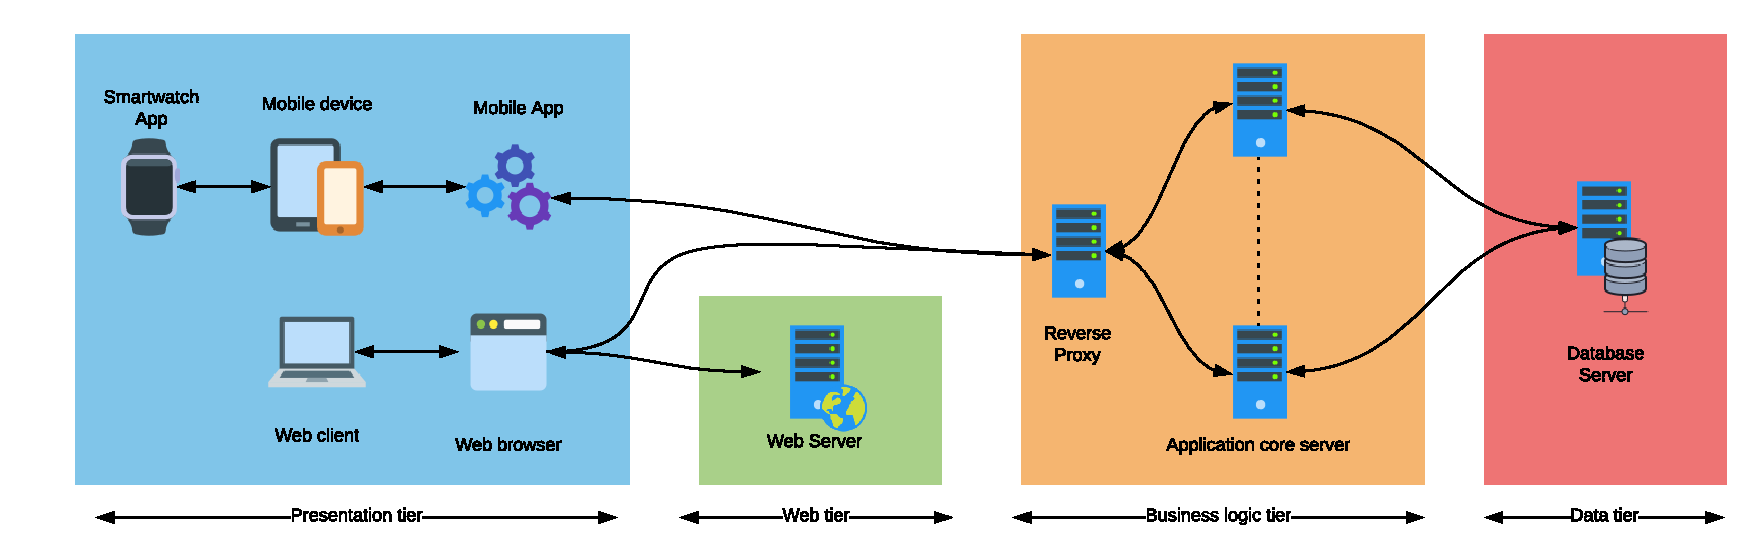
\includegraphics[width=\textwidth,height=\textheight,keepaspectratio]{assets/MultiTierSystem.pdf}
	\caption{Multitier view of the system}
	\label{fig:MultiTierSystem}
\end{figure}

\subsubsection{Thin client}
The system will use a Thin client paradigm that will handle only communications with the main server.
Using a Fat client paradigm is not convenient in this case because our customers rely mostly on Mobile phones which can have troubles in handle computational effort.
The server of Data4Help will have sufficient computational power to manage a lot of user requests at the same time.

\subsubsection{RESTful}
The communication between the Core and the smartwatch App / Web site is made using a RESTful (Representational State Transfer) service, that means that all the query are simple HTTP query, so a security layer can be easily added using SSL/HTTPS. Moreover, the RESTful was formalized with scalability in mind, so that a web service implemented using a RESTful architecture can be easily expanded to fulfill new needs.
Being a simple HTTP request, it is compatible with all firewall/proxy, simplifying the configuration aspects of the system, and as the response body JSON can be used, a fully standardized and powerful but simple language to exchange data.

        \subsection{Other design decisions}
            \subsubsection{Model View Presenter}
The structure imposed by the chosen multi-tier architecture suggests the use of the \textbf{MVP} (Model-View-Presenter) architectural pattern.\\
Here are briefly presented the concept behind the \textbf{MVP} architecture, with respect to the component used in the service.
\begin{itemize}
    \item \textbf{Model}: Handles the communication with the database.
    \item \textbf{View}: Handles the information displayed to the generic user, therefore being, in this situation, completely passive.
    \item \textbf{Presenter}: Serves as a middleware manipulating data exposed via queries by the \textbf{Model} in response to events dispatched by a generic user (e.g Login, request for subscription etc)
\end{itemize}
\begin{center}
    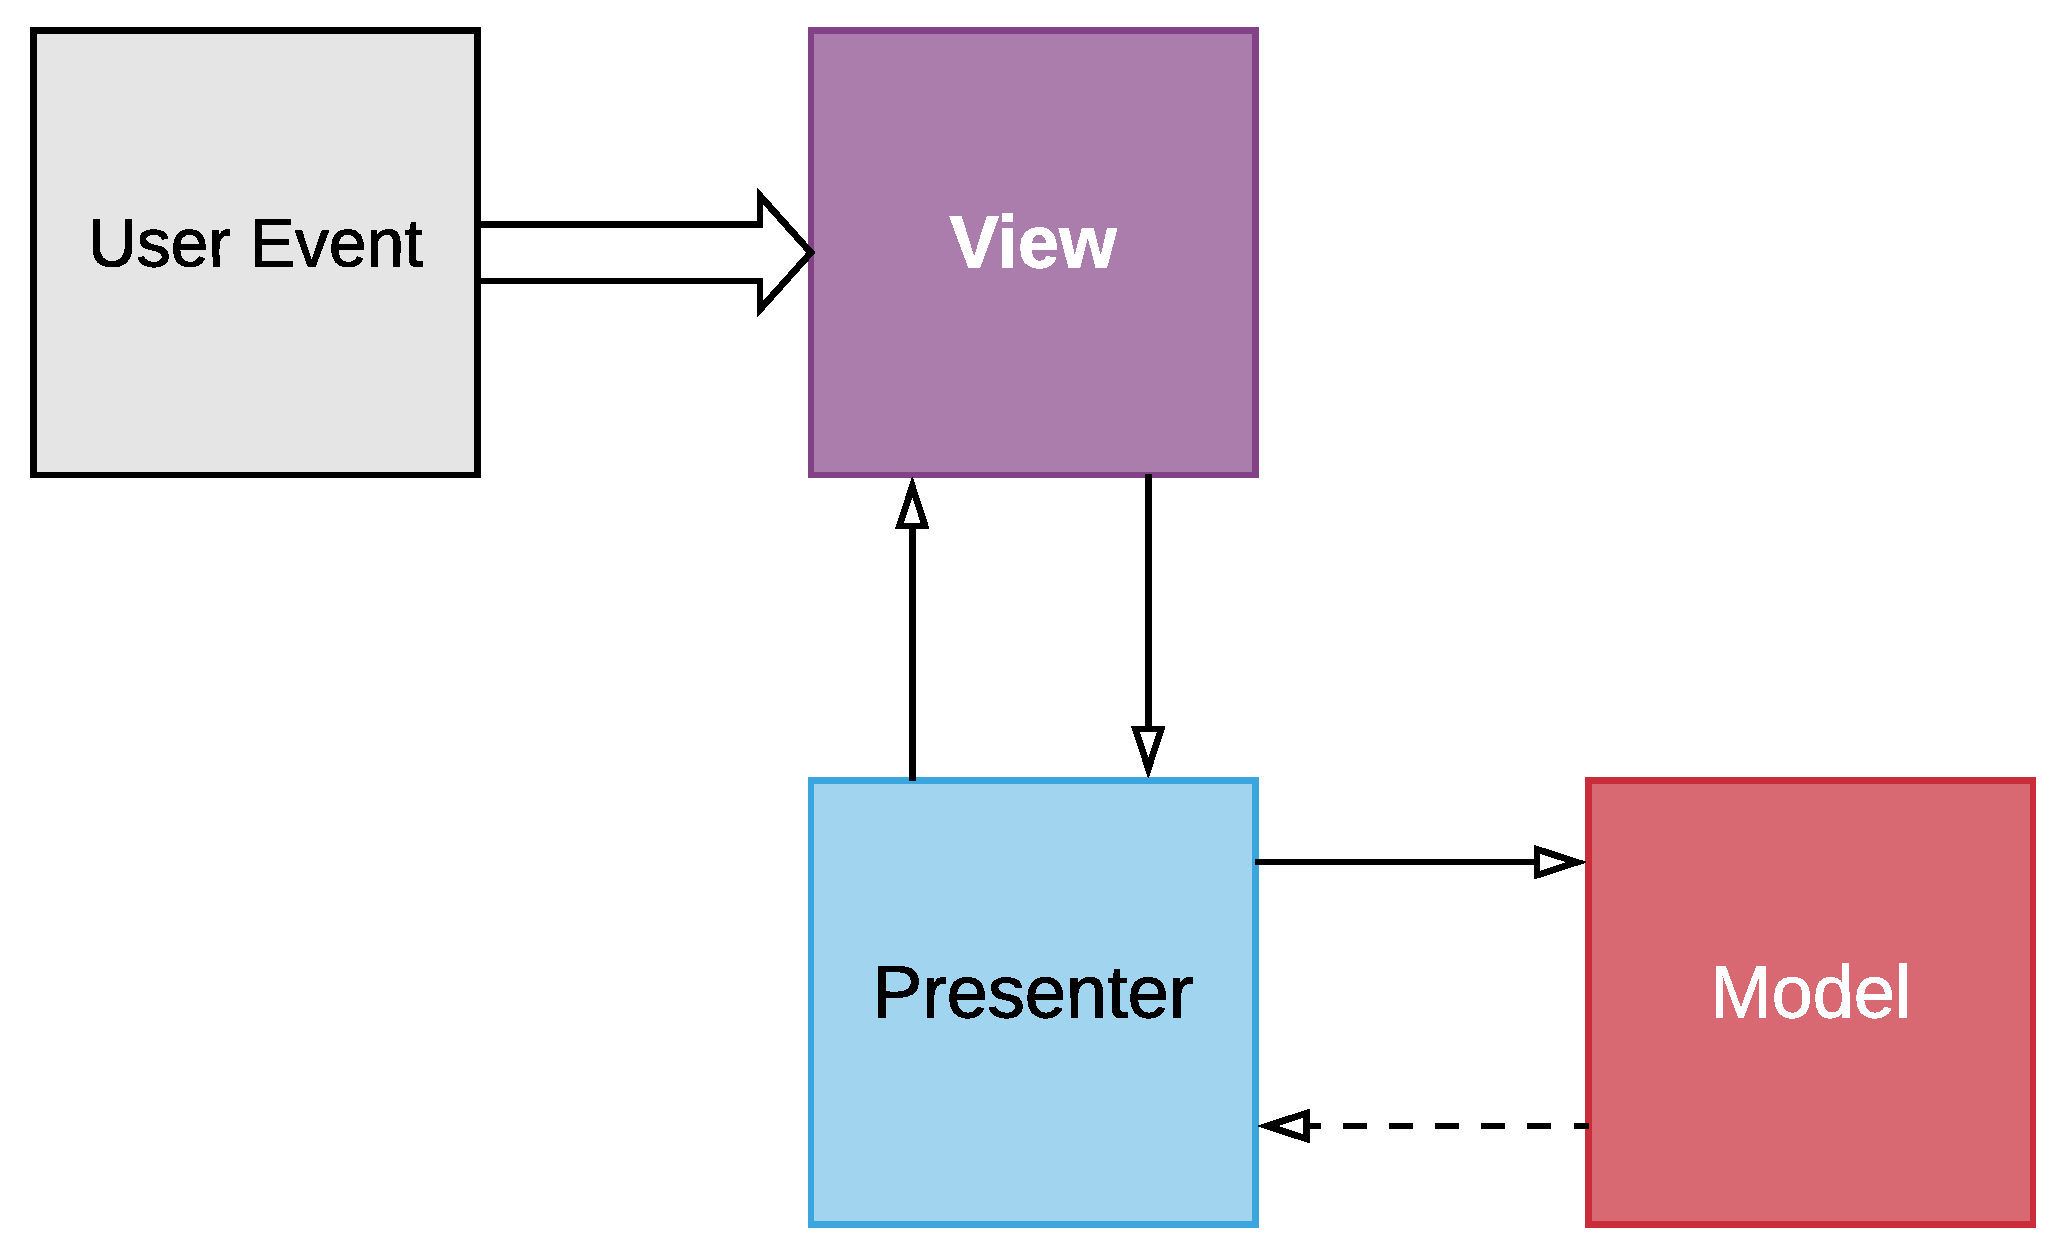
\includegraphics[width=0.5\textwidth]{assets/MVP.pdf}
\end{center}

\subsubsection{Stateless}
In order to easily serve more or less users according to the demand of the service it has been opted for a stateless \textit{Business Logic Tier}. This allows the service to be scaled when needed, therefore saving resources when requests are low. 

        
    \newpage
    \section{User interface design}
        As shown in the UX Diagram below, the user must first select if he is a \textit{Run Organizer} or a \textit{Normal User}, then he can proceed in choosing wheather he wants to login or register. \\
The \textit{Login} and \textit{Registration} flow are similar, being associated with similar procedures.
The only difference is that, due to the fact that a SmartWatch is required for the \textit{Normal User} to use the app, the presence of it is checked during \textit{Login} and \textit{Registration}.
\\
If the procedures mentioned before are successful the user lands on the \textit{Main Screen}, on which a Navigation Drawer presents him the \textit{Navigation Options}.\\ \\
\noindent If the User is a \textit{Run Organizer} the options are the following: 
\begin{itemize}
    \item View All Runs
    \item Organize a Run
\end{itemize}
\vspace{0.5cm}
If the User is a \textit{Normal User} the options are the following: 
\begin{itemize}
    \item Health Graph
    \item All Runs Available
    \item AutomatedSOS
\end{itemize}

\vspace{0.5cm}
\noindent If the \textit{Run Organizer} selects the \textit{View All Runs} option he is presented with a screen in which all run organized by him are present. Tapping on a run results in a screen with all the information concerning it shown.
If the \textit{Run Organizer} selects the \textit{Organize a run} option he is presented with the \textit{Run Organization Form} screen which will be followed by, after submission, the \textit{Run Info} screen.

\vspace{0.5cm}
\noindent The \textit{Normal User} has the possibility to: 
\begin{itemize}
    \item View the \textit{Health Graph} screen, by which, tapping on a graph, results in more information concerning the selected health parameters being shown.
    \item See \textit{All Runs Available}, by which, tapping on a run, results in more informations on the run being show.
    \item Subscribe to \textit{AutomatedSOS}.
\end{itemize}

\begin{figure}
        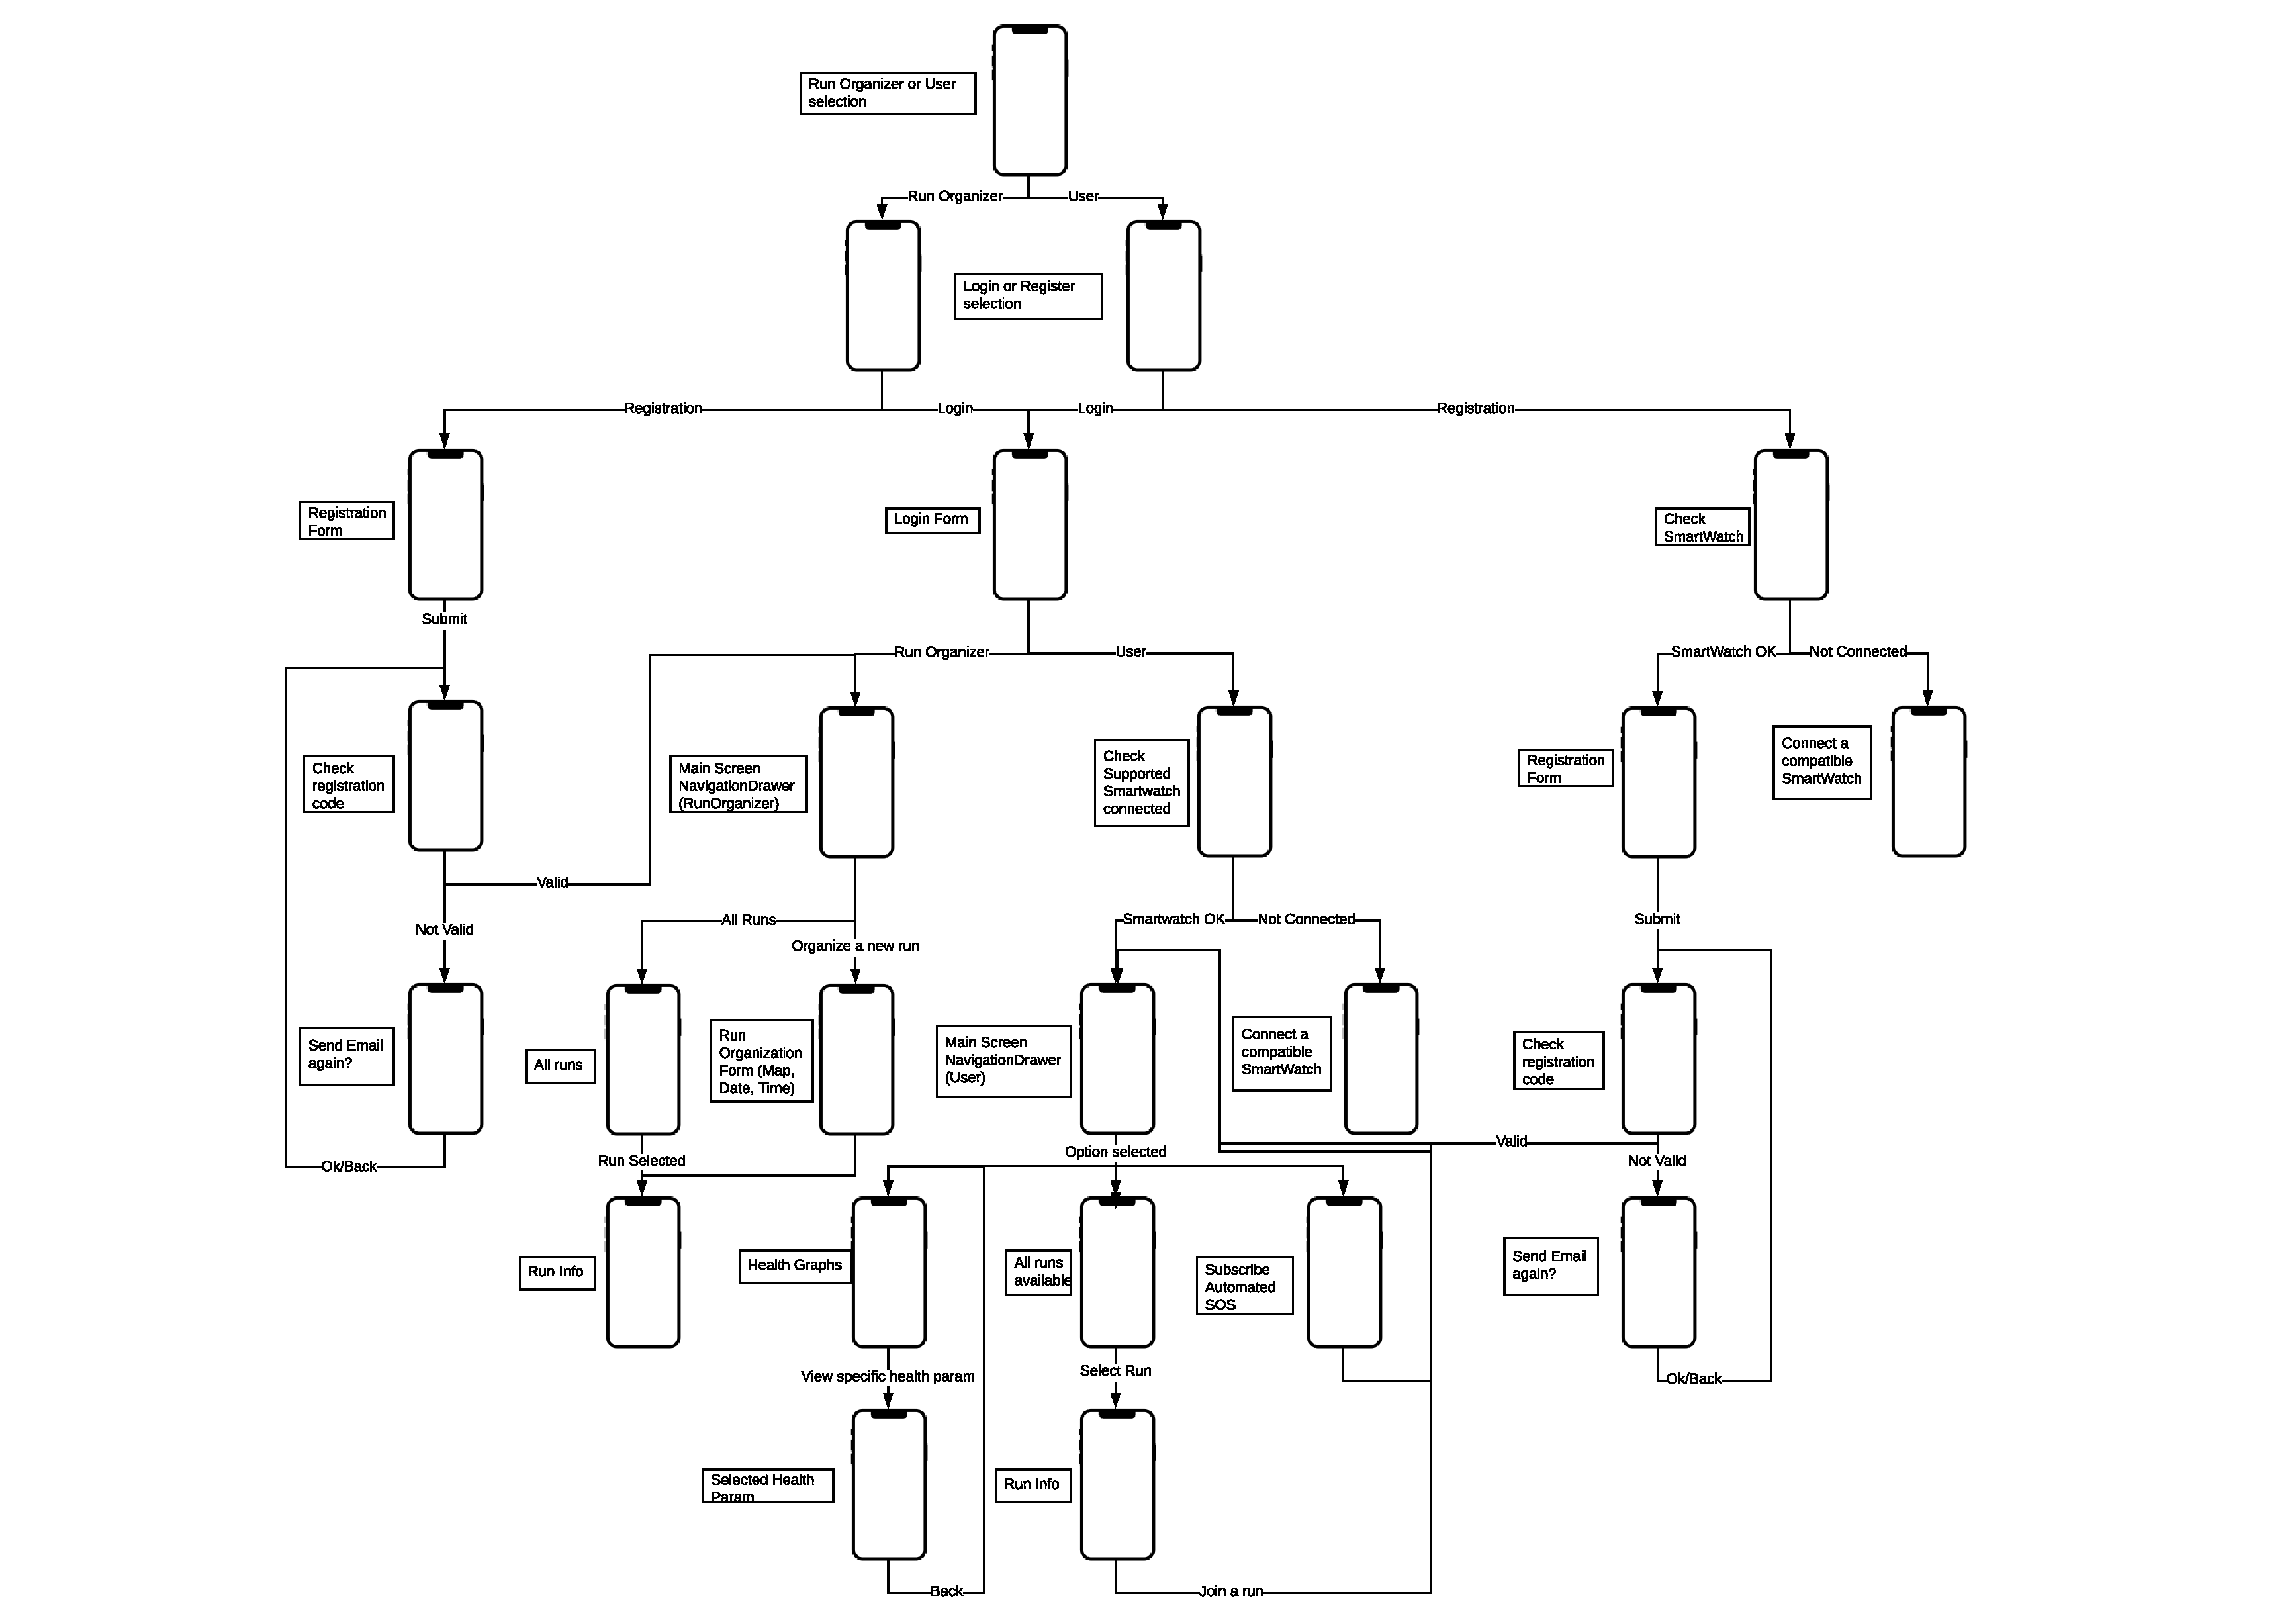
\includegraphics[width=\textwidth,height=\textheight,keepaspectratio]{assets/flowCharts/UXDiagramMobile.pdf}
    \caption{UX Diagram for Website}
    \label{fig:UXDiagram}
\end{figure}







\begin{figure}
        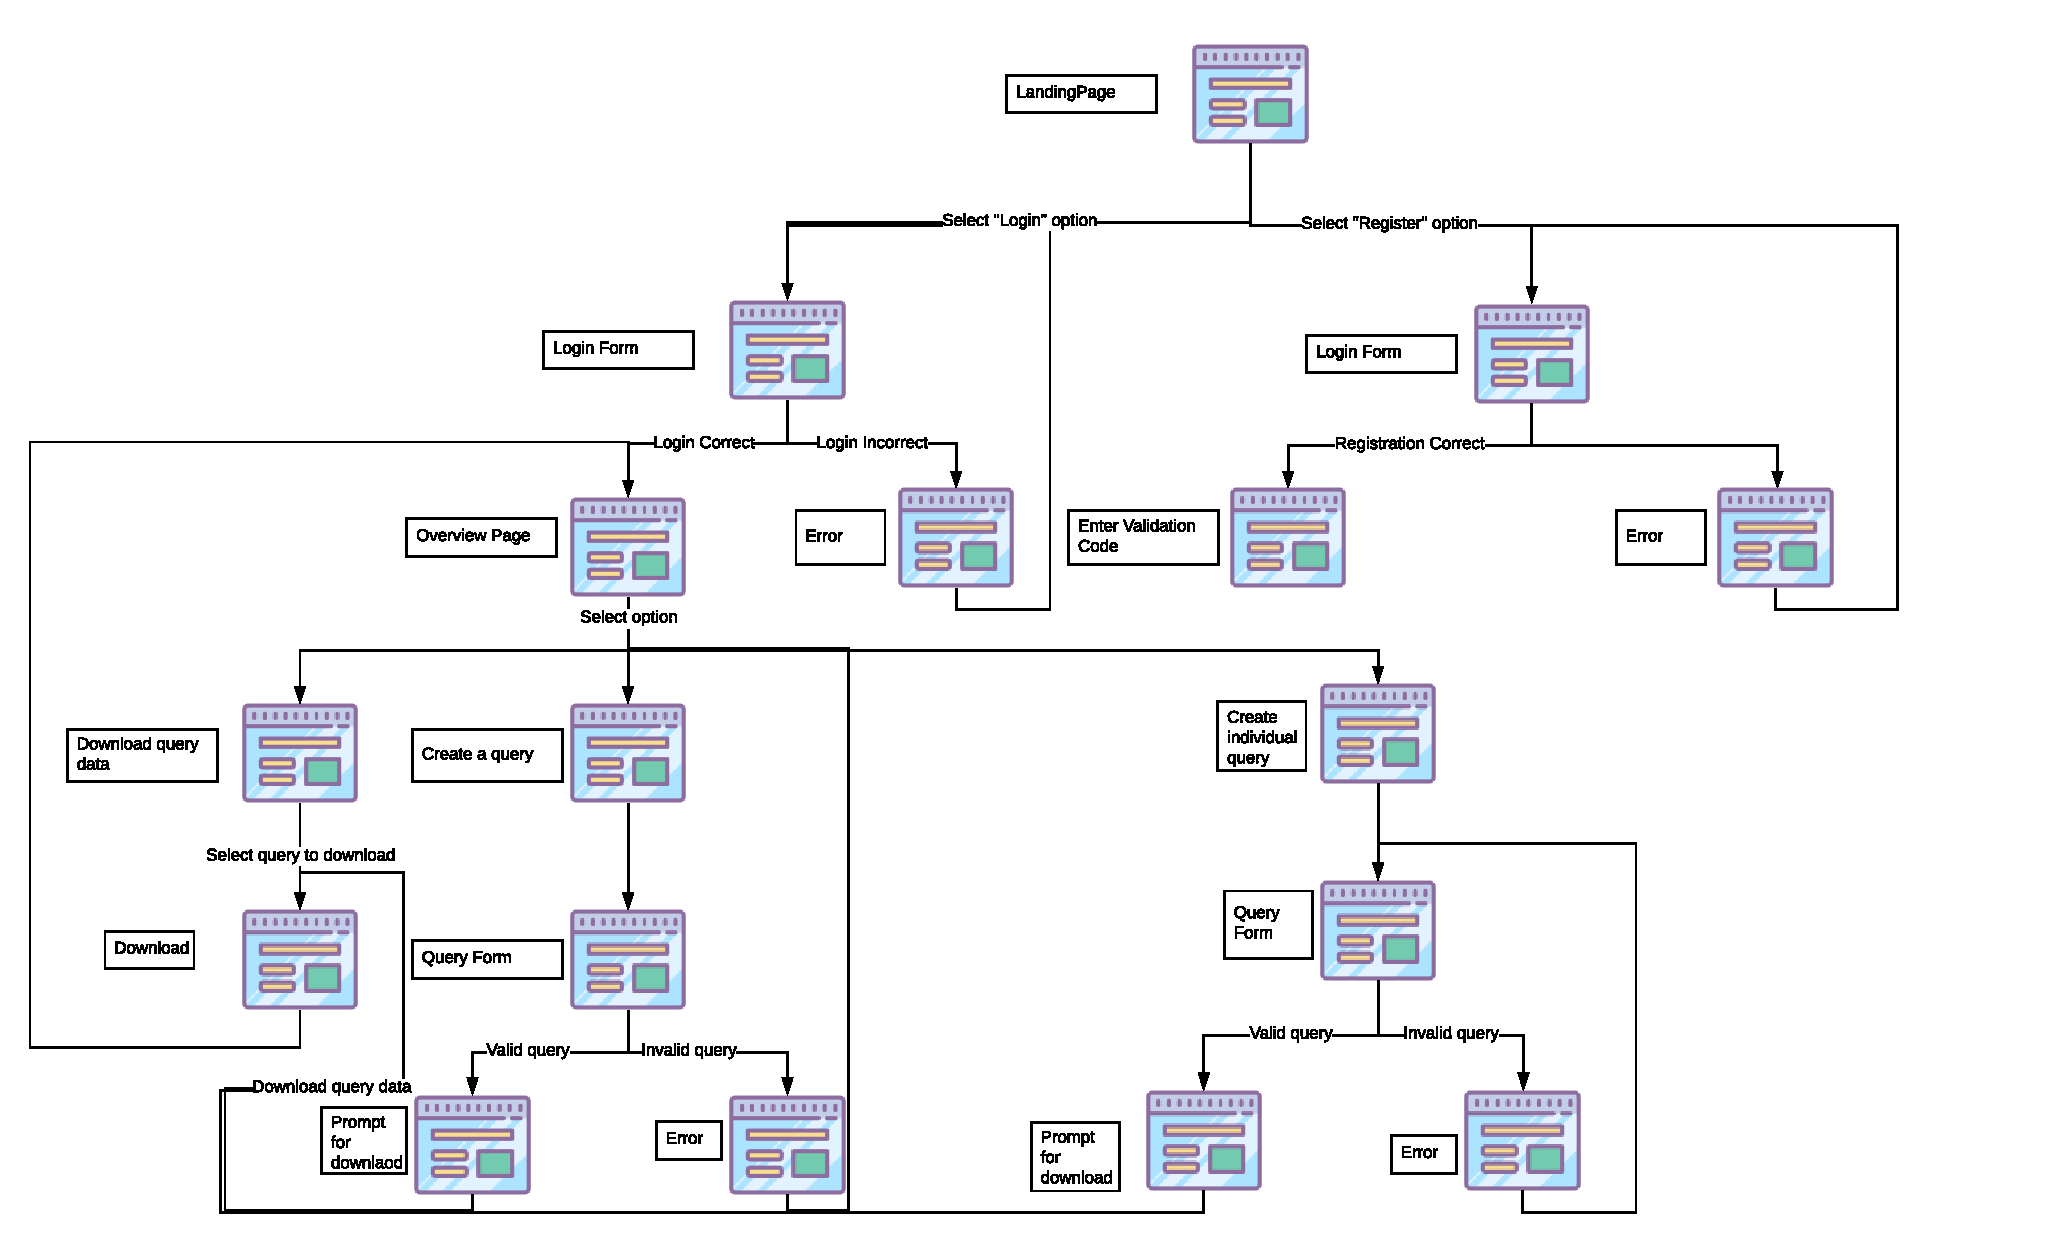
\includegraphics[width=\textwidth,height=\textheight,keepaspectratio]{assets/flowCharts/UXDiagramWebsite.pdf}
    \caption{UX Diagram for Mobile App}
    \label{fig:uxWebsite}
\end{figure}

    \newpage
    \section{Requirements traceability}
        In this paragraph is shown the mapping between every component and the requirement satisfied.

\begin{tabular}{l*{6}{c}r}
    \hline
    \textbf{Design component} &  \textbf{Requirement} \\
    \hline
    Authentication manager & \textbf{[R1$_W$]}\\
                        & \textbf{[RM$_M$]}\\
                        & \textbf{[R1$_M$]}\\
                        & \textbf{[R2$_M$]}\\
                        & \textbf{[R3$_M$]}\\
                        & \textbf{[R1$_W$]}\\
                        & \textbf{[R2$_W$]}\\
                        & \textbf{[R3$_W$]}\\
                        & \textbf{[R5$_W$]}\\
                        & \textbf{[R10$_W$]}\\
                        & \textbf{[R11$_W$]}\\
                        & \textbf{[R14$_C$]}\\
    \hline
    Individuals Manager & X   \\
                        & \textbf{[RM$_M$]}\\
                        & \textbf{[R1$_M$]}\\
                        & \textbf{[R2$_M$]}\\
                        & \textbf{[R3$_M$]}\\
                        & \textbf{[R1$_W$]}\\
                        & \textbf{[R2$_W$]}\\
                        & \textbf{[R3$_W$]}\\
                        & \textbf{[R5$_W$]}\\
                        & \textbf{[R10$_W$]}\\
                        & \textbf{[R11$_W$]}\\
                        & \textbf{[R14$_C$]}\\
    \hline
    Query Manager & X   \\ 
                        & \textbf{[RM$_M$]}\\
                        & \textbf{[R1$_M$]}\\
                        & \textbf{[R2$_M$]}\\
                        & \textbf{[R3$_M$]}\\
                        & \textbf{[R1$_W$]}\\
                        & \textbf{[R2$_W$]}\\
                        & \textbf{[R3$_W$]}\\
                        & \textbf{[R5$_W$]}\\
                        & \textbf{[R10$_W$]}\\
                        & \textbf{[R11$_W$]}\\
                        & \textbf{[R14$_C$]}\\

    \hline
    Subscription Manager & X   \\
                        & \textbf{[RM$_M$]}\\
                        & \textbf{[R1$_M$]}\\
                        & \textbf{[R2$_M$]}\\
                        & \textbf{[R3$_M$]}\\
                        & \textbf{[R1$_W$]}\\
                        & \textbf{[R2$_W$]}\\
                        & \textbf{[R3$_W$]}\\
                        & \textbf{[R5$_W$]}\\
                        & \textbf{[R10$_W$]}\\
                        & \textbf{[R11$_W$]}\\
                        & \textbf{[R14$_C$]}\\
    \hline
    Emergency Manager & X   \\
                        & \textbf{[RM$_M$]}\\
                        & \textbf{[R1$_M$]}\\
                        & \textbf{[R2$_M$]}\\
                        & \textbf{[R3$_M$]}\\
                        & \textbf{[R1$_W$]}\\
                        & \textbf{[R2$_W$]}\\
                        & \textbf{[R3$_W$]}\\
                        & \textbf{[R5$_W$]}\\
                        & \textbf{[R10$_W$]}\\
                        & \textbf{[R11$_W$]}\\
                        & \textbf{[R14$_C$]}\\
    \hline
    Run Manager & X   \\
                        & \textbf{[RM$_M$]}\\
                        & \textbf{[R1$_M$]}\\
                        & \textbf{[R2$_M$]}\\
                        & \textbf{[R3$_M$]}\\
                        & \textbf{[R1$_W$]}\\
                        & \textbf{[R2$_W$]}\\
                        & \textbf{[R3$_W$]}\\
                        & \textbf{[R5$_W$]}\\
                        & \textbf{[R10$_W$]}\\
                        & \textbf{[R11$_W$]}\\
                        & \textbf{[R14$_C$]}\\
    \hline
    Push Notification Interface & X   \\
                        & \textbf{[RM$_M$]}\\
                        & \textbf{[R1$_M$]}\\
                        & \textbf{[R2$_M$]}\\
                        & \textbf{[R3$_M$]}\\
                        & \textbf{[R1$_W$]}\\
                        & \textbf{[R2$_W$]}\\
                        & \textbf{[R3$_W$]}\\
                        & \textbf{[R5$_W$]}\\
                        & \textbf{[R10$_W$]}\\
                        & \textbf{[R11$_W$]}\\
                        & \textbf{[R14$_C$]}\\
    \hline
    Emergency Services Interface & X \\
                        & \textbf{[RM$_M$]}\\
                        & \textbf{[R1$_M$]}\\
                        & \textbf{[R2$_M$]}\\
                        & \textbf{[R3$_M$]}\\
                        & \textbf{[R1$_W$]}\\
                        & \textbf{[R2$_W$]}\\
                        & \textbf{[R3$_W$]}\\
                        & \textbf{[R5$_W$]}\\
                        & \textbf{[R10$_W$]}\\
                        & \textbf{[R11$_W$]}\\
                        & \textbf{[R14$_C$]}\\
    \hline
    Mail Services Interface & X \\
                        & \textbf{[RM$_M$]}\\
                        & \textbf{[R1$_M$]}\\
                        & \textbf{[R2$_M$]}\\
                        & \textbf{[R3$_M$]}\\
                        & \textbf{[R1$_W$]}\\
                        & \textbf{[R2$_W$]}\\
                        & \textbf{[R3$_W$]}\\
                        & \textbf{[R5$_W$]}\\
                        & \textbf{[R10$_W$]}\\
                        & \textbf{[R11$_W$]}\\
                        & \textbf{[R14$_C$]}\\
    
\end{tabular}
    \newpage
    \section{Implementation, integration and test plan}
        As previously mentioned in this document, the System can be divided into three main part: the Core, the Website and the Mobile App + Smartwatch App. More specifically:
\begin{itemize}
    \item \textbf{Frontend components:} contains the Smartwatch App, the Mobile App and the Website.
    \item \textbf{Backend components:} contains the Core with all its components and the DBMS.
    \item \textbf{External components:} contains all the external components, such as the Payment Service, the communication with the Ambulance system and so on.
\end{itemize}

\noindent In order to implement, integrate and test the system, a \textit{Bottom-up approach} will be used. In this way, the different subsystems can be implemented independently one from each other. As the dependencies of each subsystem are developed, the various subsystems can be progressively integrated and tested.\\
For what concerning the Mobile App and the Website, these can be implemented assuming that the Core is fully working and running, as they interact only using REST api (i.e. a stub server with mockup responses can be used as these are fully formalized in this document). Only when the Core is fully developed and tested an integration test can be made.

The components to be implemented, integrated and tested are, in order:
\begin{enumerate}
    \item DBMS \& Storage Manager;
    \item Authentication Manager, along with Mail interface;
    \item Individual Manager, along with Push Notification interface;
    \item Subscription Manager, along with the Payment interface;
    \item Query Manager, with integration with Push Notification;
    \item Emergency Manager, along with Emergency interface;
    \item Run Manager, with integration with Individual manager.
\end{enumerate}

\label{CD}

As the Core integration and testing is finished, the integration between the Website and the Core and the Smartphone App and the Core can be made in this order:
\begin{enumerate}
    \item Website, Mobile App with Authentication manager;
    \item Mobile App with Individual manager;
    \item Website with Subscription manager;
    \item Website with Query manager;
    \item Mobile App with Run manager.
\end{enumerate}













\subsection{Sequence of component integration}
The diagrams below describe the sequence of the component implementation, integration and testing of the system.

\paragraph{Integration of the backend}
Firstly all the components will be implemented and tested with unit tests.
Database and Storage manager are the firsts to be implemented and tested because they offer methods to access data.
Then the integration process will proceed in the following order:





\begin{figure}[H]
	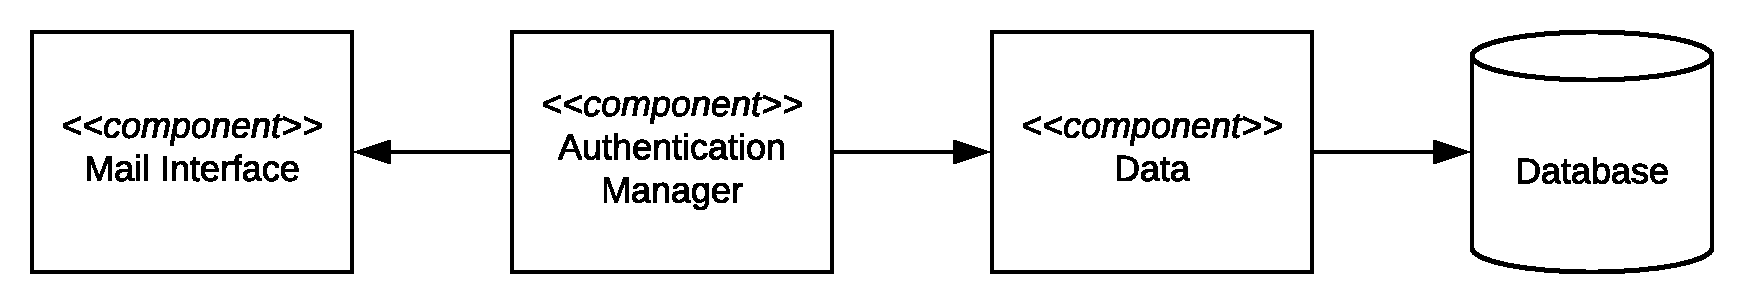
\includegraphics[width=\textwidth,height=\textheight,keepaspectratio]{assets/integration/AuthDataMail.pdf}
	\caption{Auth Manager integration}
	\label{fig:AuthDataMail}
\end{figure}



\begin{figure}[H]
	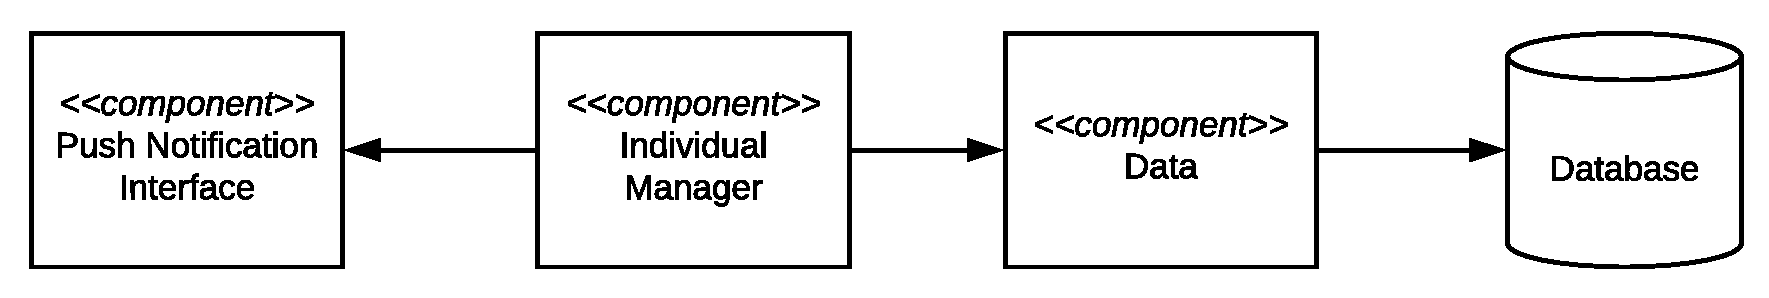
\includegraphics[width=\textwidth,height=\textheight,keepaspectratio]{assets/integration/IndividualPush.pdf}
	\caption{Individual Manager integration}
	\label{fig:IndividualPush}
\end{figure}

\begin{figure}[H]
	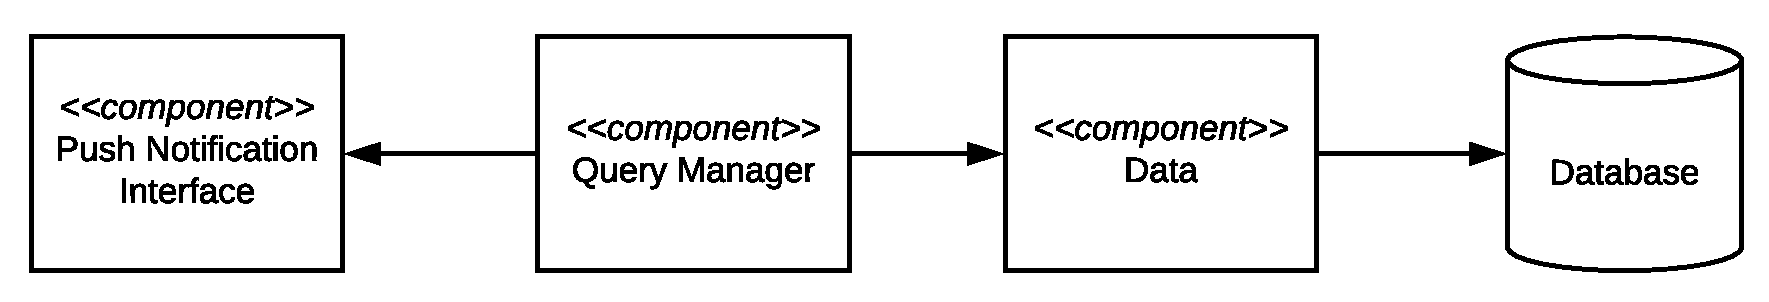
\includegraphics[width=\textwidth,height=\textheight,keepaspectratio]{assets/integration/QueryPush.pdf}
	\caption{Query Manager integration}
	\label{fig:QueryPush}
\end{figure}



\begin{figure}[H]
	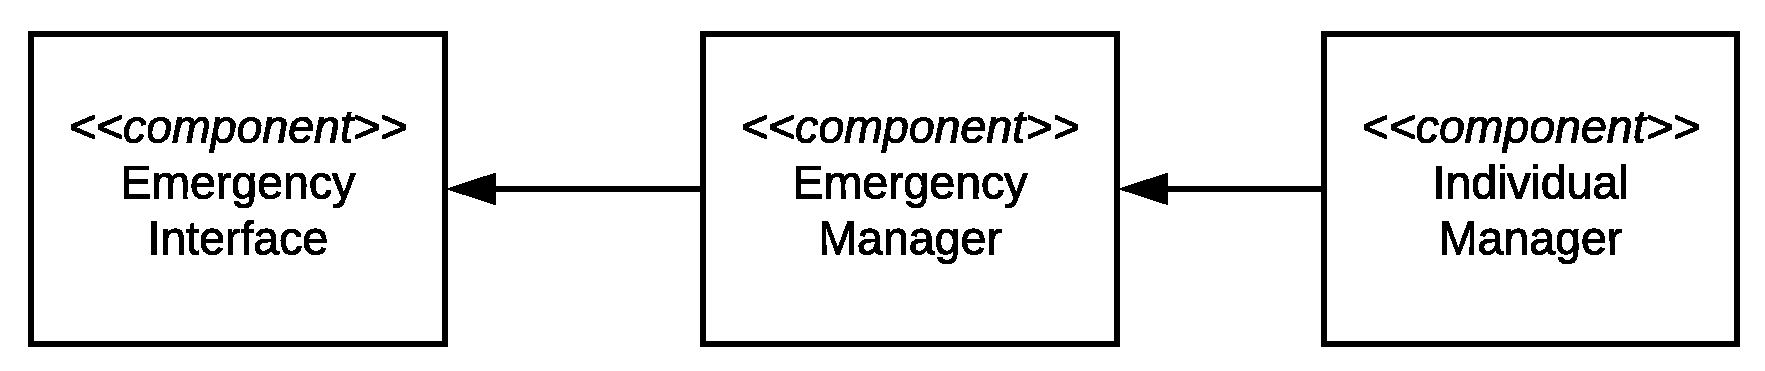
\includegraphics[width=\textwidth,height=\textheight,keepaspectratio]{assets/integration/EmergencyIndividual.pdf}
	\caption{Emergencency Manager integration}
	\label{fig:EmergencyIndividual}
\end{figure}


\begin{figure}[H]
	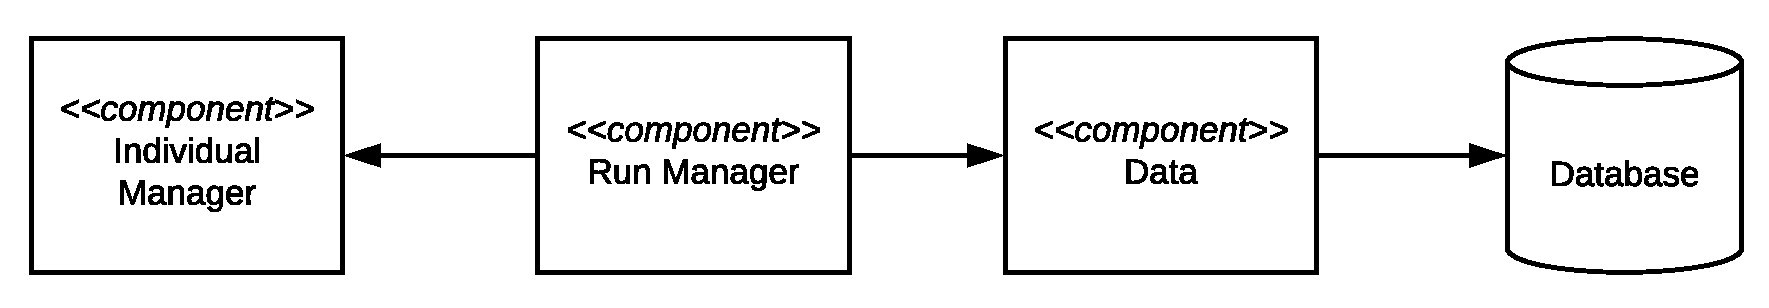
\includegraphics[width=\textwidth,height=\textheight,keepaspectratio]{assets/integration/IndividualRun.pdf}
	\caption{Run Manager Integration}
	\label{fig:IndividualRun}
\end{figure}

\noindent In order to have the main functionality tested, we expect to integrate the external interfaces at the same time with the integration with other internal components.




\paragraph{Integration of the frontend with backend}
Once all the components of the backend are implemented and tested among each others, the frontend will be integrated and tested within the backend. \\
The subsystems to be integrated are 2:
\begin{itemize}
    \item The Website Client, that interacts with the Authentication Manager, Query Manager, Subscription Manager;
    \item The Mobile app Client, that interacts with the Run Manager, Authentication Manager, and Individual Manager
\end{itemize}

\begin{figure}[H]
	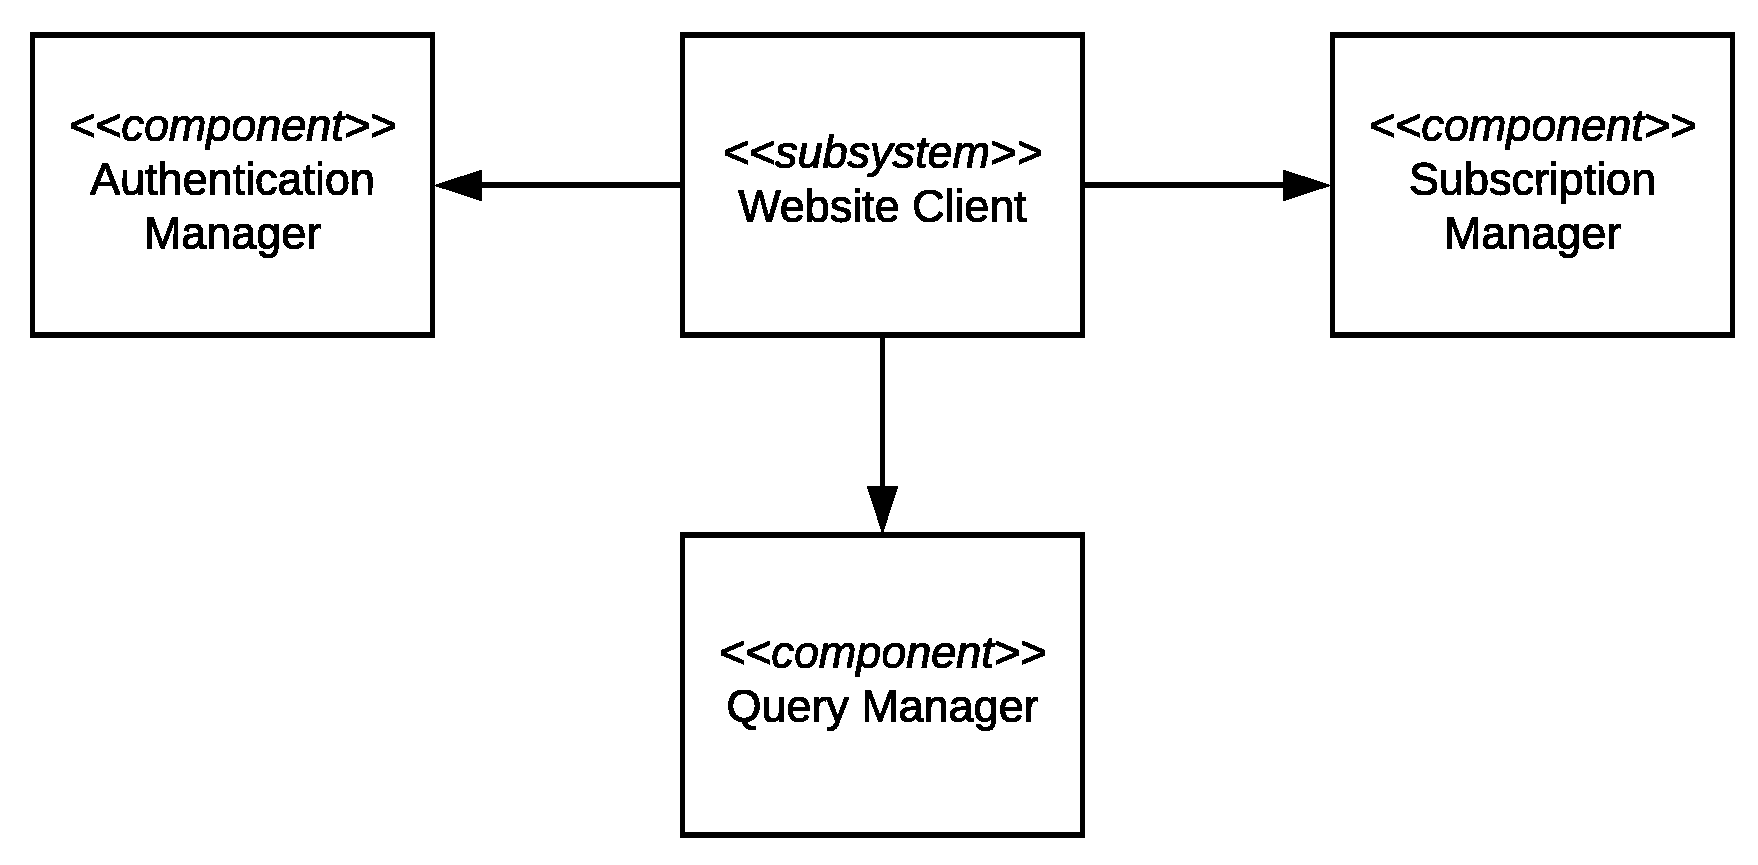
\includegraphics[width=\textwidth,height=\textheight,keepaspectratio]{assets/integration/IntegrationWebsite.pdf}
	\caption{Website integration}
	\label{fig:IntegrationWebsite}
\end{figure}

\begin{figure}[H]
	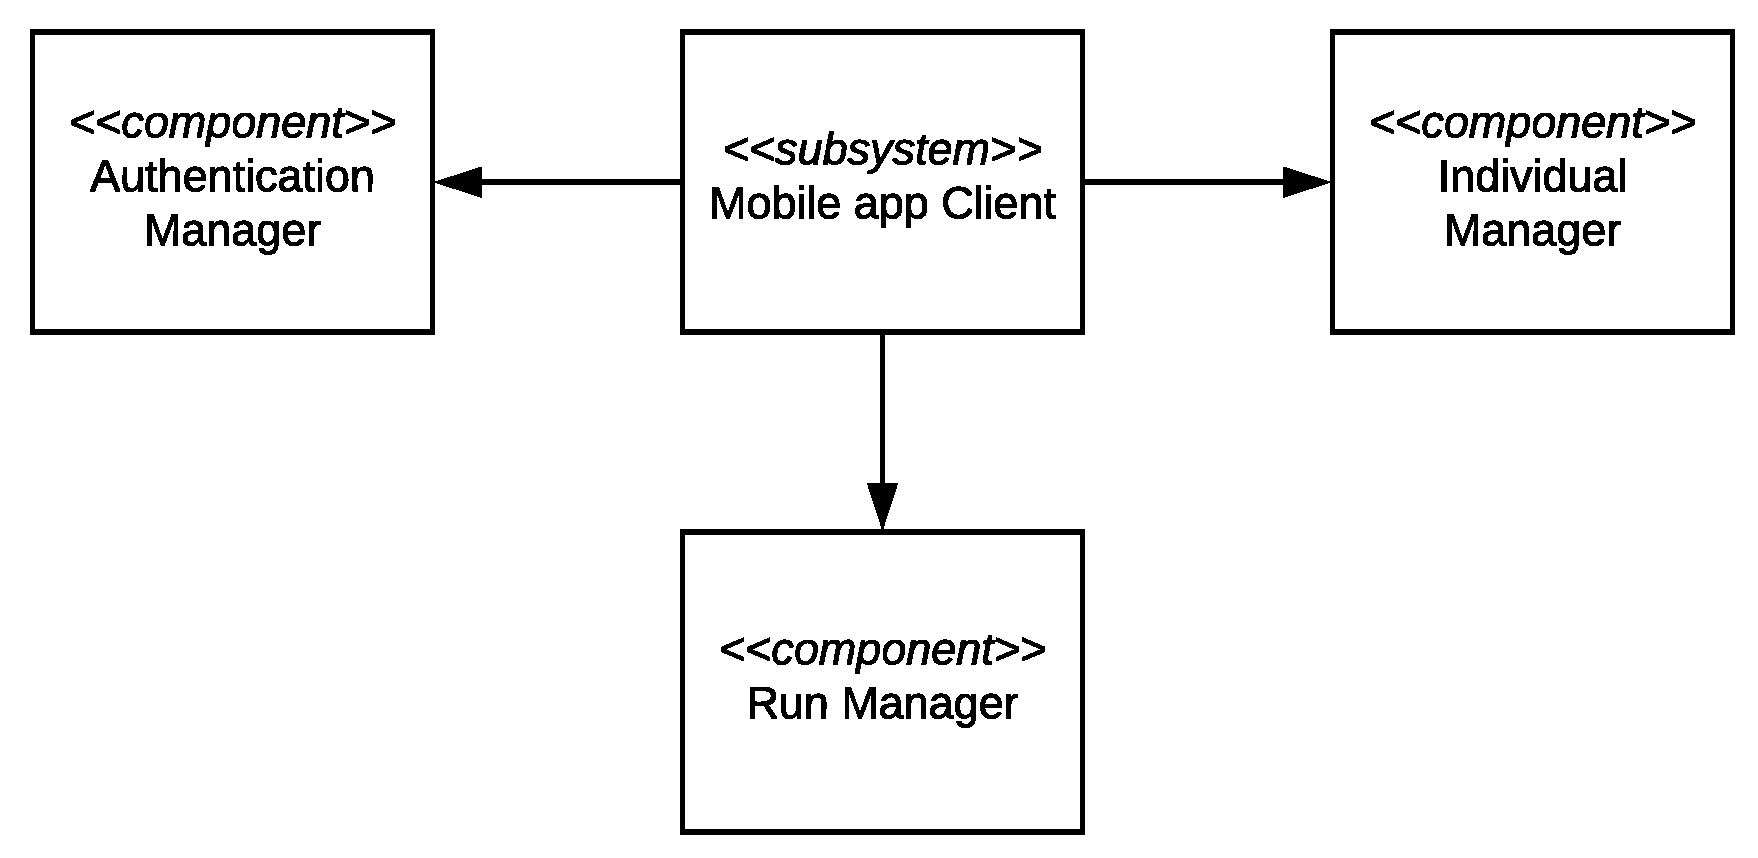
\includegraphics[width=\textwidth,height=\textheight,keepaspectratio]{assets/integration/IntegrationMobileApp.pdf}
	\caption{Mobile App integration}
	\label{fig:IntegrationMobileApp}
\end{figure}


\paragraph{Integration of all subsystems}
Once the front-end has been integrated with the Back-end, the system will be fully tested, with the respect of all the components shown in the \nameref{fig:CD}.


    \newpage
    \subsection{Effort spent}
        \input{chapters/6.EffortSpent.tex}
    \newpage
    \subsection{References}
        \input{chapters/7.References.tex}
        
    \section{Hours tracking}
        \begin{tabular}{l*{6}{c}r}
            Date & Nicola Fossati & Daniele Montesi & Francesco Sgherzi \\
            \hline
            13/11/2018 & 2 & 0 & 0   \\
            \hline
            19/11/2018 & 2 & 5 & 3   \\
            \hline
            20/11/2018 & 3 & 3 & 0   \\
            \hline
            21/11/2018 & 2 & 2 & 0   \\
            \hline
            22/11/2018 & 3 & 3 & 0   \\
            \hline
            23/11/2018 & 4 & 4 & 0   \\
            \hline
            26/11/2018 & 3 & 3 & 6   \\
            \hline
            27/11/2018 & 4 & X & X   \\
        \end{tabular}
\end{document}